% option draft um zu lange Zeilen anzuzeigen
\documentclass[a4paper,11pt]{book}

\usepackage[english]{babel}
\usepackage[utf8]{inputenc}
\usepackage[T1]{fontenc}
\usepackage[inner=3.5cm,top=3cm,outer=3cm,bottom=3cm]{geometry}
\usepackage{color}
\usepackage[xindy,toc]{glossaries}	% before hyperref to prevent links
\usepackage{hyperref}
\usepackage{listings}
\usepackage{url}
\usepackage{setspace}
\usepackage{graphicx}
\usepackage[intoc]{nomencl}
\usepackage{titletoc}
\usepackage[noindentafter]{titlesec}
\usepackage{verbatim}
\usepackage{array}
\usepackage{amsmath}
\usepackage{amssymb}
\usepackage[table]{xcolor}
\usepackage{paralist}

\usepackage[numbers]{natbib}
\bibliographystyle{unsrtnat-lastchecked}

% empty header, page-numbers in footer
\usepackage{fancyhdr}
\lhead{}
\chead{}
\rhead{}
\lfoot{}
\cfoot{\thepage}
\renewcommand{\headrulewidth}{0pt}
\rfoot{}

% to place pictures with [H] at a specific position
\usepackage{float}
\restylefloat{figure}

% length of paragraph indent
\setlength{\parindent}{10pt}

% colors
\definecolor{kwColor}{rgb}{0.49,0,0.33}
\definecolor{identColor}{rgb}{0,0,0}
\definecolor{commentColor}{rgb}{0,.5,0}
\definecolor{iLinkColor}{rgb}{0,0,.4}
\definecolor{eLinkColor}{rgb}{0.7,0,0}
%\definecolor{iLinkColor}{rgb}{0,0,0}
%\definecolor{eLinkColor}{rgb}{0,0,0}
\definecolor{stringColor}{rgb}{0,0,0.8}

% setup
\hypersetup{
	bookmarks=true,
	pdfnewwindow=true,
	colorlinks=true,
	linkcolor=iLinkColor,
	citecolor=iLinkColor,
	filecolor=iLinkColor,
	urlcolor=eLinkColor
}

% highlighting for mmix-asm
\lstdefinelanguage{mmixal}{
	morekeywords={
		TRAP, FCMP, FUN, FEQL, FADD, FIX, FSUB, FIXU,
		FLOT, FLOTI, FLOTU, FLOTUI, SFLOT, SFLOTI, SFLOTU, SFLOTUI,
		FMUL, FCMPE, FUNE, FEQLE, FDIV, FSQRT, FREM, FINT,
		MUL, MULI, MULU, MULUI, DIV, DIVI, DIVU, DIVUI,
		ADD, ADDI, ADDU, ADDUI, SUB, SUBI, SUBU, SUBUI,
		IIADDU, IIADDUI, IVADDU, IVADDUI, VIIIADDU, VIIIADDUI, XVIADDU, XVIADDUI,
		CMP, CMPI, CMPU, CMPUI, NEG, NEGI, NEGU, NEGUI,
		SL, SLI, SLU, SLUI, SR, SRI, SRU, SRUI,
		BN, BNB, BZ, BZB, BP, BPB, BOD, BODB,
		BNN, BNNB, BNZ, BNZB, BNP, BNPB, BEV, BEVB,
		PBN, PBNB, PBZ, PBZB, PBP, PBPB, PBOD, PBODB,
		PBNN, PBNNB, PBNZ, PBNZB, PBNP, PBNPB, PBEV, PBEVB,
		CSN, CSNI, CSZ, CSZI, CSP, CSPI, CSOD, CSODI,
		CSNN, CSNNI, CSNZ, CSNZI, CSNP, CSNPI, CSEV, CSEVI,
		ZSN, ZSNI, ZSZ, ZSZI, ZSP, ZSPI, ZSOD, ZSODI,
		ZSNN, ZSNNI, ZSNZ, ZSNZI, ZSNP, ZSNPI, ZSEV, ZSEVI,
		LDB, LDBI, LDBU, LDBUI, LDW, LDWI, LDWU, LDWUI,
		LDT, LDTI, LDTU, LDTUI, LDO, LDOI, LDOU, LDOUI,
		LDSF, LDSFI, LDHT, LDHTI, CSWAP, CSWAPI, LDUNC, LDUNCI,
		LDVTS, LDVTSI, PRELD, PRELDI, PREGO, PREGOI, GO, GOI,
		STB, STBI, STBU, STBUI, STW, STWI, STWU, STWUI,
		STT, STTI, STTU, STTUI, STO, STOI, STOU, STOUI,
		STSF, STSFI, STHT, STHTI, STCO, STCOI, STUNC, STUNCI,
		SYNCD, SYNCDI, PREST, PRESTI, SYNCID, SYNCIDI, PUSHGO, PUSHGOI,
		OR, ORI, ORN, ORNI, NOR, NORI, XOR, XORI,
		AND, ANDI, ANDN, ANDNI, NAND, NANDI, NXOR, NXORI,
		BDIF, BDIFI, WDIF, WDIFI, TDIF, TDIFI, ODIF, ODIFI,
		MUX, MUXI, SADD, SADDI, MOR, MORI, MXOR, MXORI,
		SETH, SETMH, SETML, SETL, INCH, INCMH, INCML, INCL,
		ORH, ORMH, ORML, ORL, ANDNH, ANDNMH, ANDNML, ANDNL,
		JMP, JMPB, PUSHJ, PUSHJB, GETA, GETAB, PUT, PUTI,
		POP, RESUME, SAVE, UNSAVE, SYNC, SWYM, GET, TRIP,
		LOC, BYTE, WYDE, TETRA, OCTA
	},
	sensitive=true,
	morecomment=[l]{\%},
}
% don't use any highlighting
\lstdefinelanguage{plain}{
}
% a language for GIMMIX, based on ANSI-C, with a few more keywords for better readability
\lstdefinelanguage{GIMMIXC}[ANSI]{C}{
	morekeywords={octa,tetra,wyde,byte,bool}
}
% default-highlighting
\lstset{
	language=plain,
	framesep=5pt,
	basicstyle=\ttfamily\normalsize,
	keywordstyle=\color{kwColor}\bfseries,
	identifierstyle=\color{identColor}, 
	commentstyle=\color{commentColor},
	stringstyle=\color{stringColor},
	showstringspaces=false,
	frame=tb,
	columns=fixed,
	tabsize=4,
	breaklines=true,
	captionpos=b,
}
% for using `...` instead of \lstinline`...`
\lstMakeShortInline`

% fix for \lstlistoflistings. source: http://www.komascript.de/node/477
\makeatletter
\@ifundefined{float@listhead}{}{%
    \renewcommand*{\lstlistoflistings}{%
        \begingroup
    	    \if@twocolumn
                \@restonecoltrue\onecolumn
            \else
                \@restonecolfalse
            \fi
            \float@listhead{\lstlistlistingname}%
            \setlength{\parskip}{\z@}%
            \setlength{\parindent}{\z@}%
            \setlength{\parfillskip}{\z@ \@plus 1fil}%
            \@starttoc{lol}%
            \if@restonecol\twocolumn\fi
        \endgroup
    }%
}
\makeatother

% number subsubsections and add to toc
\setcounter{secnumdepth}{3}
\setcounter{tocdepth}{3}

% paragraphs look like subsubsubsections
\titleformat{\paragraph}[hang]{\bf}{\thetitle\quad}{0pt}{}
\titlespacing{\paragraph}{0pt}{1em}{0.5em}

% subparagraphs look like paragraphs
\titleformat{\subparagraph}[runin]{\bf}{}{0.5em}{}
\titlespacing{\subparagraph}{0pt}{1em}{1em}

% begin sections, tables and pictures with 1
\renewcommand*\thesection{\arabic{section}}
\renewcommand{\thetable}{\arabic{table}}
\renewcommand\thefigure{\arabic{figure}}

% a few convenience commands
\renewcommand{\b}[1]{\textbf{#1}}
\renewcommand{\i}[1]{\emph{#1}}
\newcommand{\ie}{i.\,e. }
\newcommand{\eg}{e.\,g. }

% dynamic register
\newcommand{\dr}[1]{{\tt \$#1}}
% special register
\newcommand{\sr}[1]{{\tt r#1}}
\newcommand{\spr}[1]{{\em sp}{\tt [#1]}}
\newcommand{\sprm}[1]{sp{\tt [#1]}}
% reg or immediate
\newcommand{\sdrim}[1]{$s(\dr{#1})${\tt|#1}}
\newcommand{\sdrimm}[1]{s(\dr{#1}){\tt|#1}}
\newcommand{\udrim}[1]{\dr{#1}{\tt|#1}}
% hex-address
\newcommand{\haddr}[1]{\lstinline`\##1`}
\newcommand{\haddrt}[2]{\lstinline`\##1`\,\lstinline`#2`}
\newcommand{\haddro}[4]{\lstinline`\##1`\,\lstinline`#2`\,\lstinline`#3`\,\lstinline`#4`}
% memory access
\newcommand{\vmem}[2]{$\mbox{$\text{M}_{#1}[#2]$}$}
\newcommand{\vmemh}[2]{$\mbox{$\text{M}_{#1}[$\lstinline`\##2`$]$}$}
\newcommand{\pmem}[2]{$\mbox{$\text{m}_{#1}[#2]$}$}
\newcommand{\pmemh}[2]{$\mbox{$\text{m}_{#1}[$\lstinline`\##2`$]$}$}
% mmix instruction
\newcommand{\mi}[1]{{\tt #1}}
% NaN
\newcommand{\NaN}[0]{{\rm NaN}\,}
\newcommand{\NaNs}[0]{{\rm NaN}s\,}
% files and folders
\newcommand{\file}[1]{\textbf{#1}}
% gimmix cmd
\newcommand{\gcmd}[1]{{\tt #1}}

% table to describe an instruction
\newcommand{\instrtbl}[2]{
	\begin{table}[H]
		\begin{tabular}{| p{15mm} p{121mm} |}
			\hline
			\b{Name:} & #1\\
			\b{Effect:} & #2\\
			\hline
		\end{tabular}
	\end{table}
	\vspace{-12pt}
}
\newcommand{\instrtbltwo}[3]{
	\begin{table}[H]
		\begin{tabular}{| p{15mm} p{121mm} |}
			\hline
			\b{Name:} & #1\\
			\b{Effect:} & #2\\
			& #3\\
			\hline
		\end{tabular}
	\end{table}
	\vspace{-12pt}
}
\newcommand{\instrtblfour}[5]{
	\begin{table}[H]
		\begin{tabular}{| p{15mm} p{121mm} |}
			\hline
			\b{Name:} & #1\\
			\b{Effect:} & #2\\
			& #3\\
			& #4\\
			& #5\\
			\hline
		\end{tabular}
	\end{table}
	\vspace{-12pt}
}
\newcommand{\instrtblfive}[6]{
	\begin{table}[H]
		\begin{tabular}{| p{15mm} p{121mm} |}
			\hline
			\b{Name:} & #1\\
			\b{Effect:} & #2\\
			& #3\\
			& #4\\
			& #5\\
			& #6\\
			\hline
		\end{tabular}
	\end{table}
	\vspace{-12pt}
}
\newcommand{\instrtblsix}[7]{
	\begin{table}[H]
		\begin{tabular}{| p{15mm} p{121mm} |}
			\hline
			\b{Name:} & #1\\
			\b{Effect:} & #2\\
			& #3\\
			& #4\\
			& #5\\
			& #6\\
			& #7\\
			\hline
		\end{tabular}
	\end{table}
	\vspace{-12pt}
}
\newcommand{\instrtblseven}[8]{
	\begin{table}[H]
		\begin{tabular}{| p{15mm} p{121mm} |}
			\hline
			\b{Name:} & #1\\
			\b{Effect:} & #2\\
			& #3\\
			& #4\\
			& #5\\
			& #6\\
			& #7\\
			& #8\\
			\hline
		\end{tabular}
	\end{table}
	\vspace{-12pt}
}
\newcommand{\instrtbleight}[9]{
	\begin{table}[H]
		\begin{tabular}{| p{15mm} p{121mm} |}
			\hline
			\b{Name:} & #1\\
			\b{Effect:} & #2\\
			& #3\\
			& #4\\
			& #5\\
			& #6\\
			& #7\\
			& #8\\
			& #9\\
			\hline
		\end{tabular}
	\end{table}
	\vspace{-12pt}
}

% table to describe an gimmix command
\newcommand{\gcmdtbl}[2]{
	\begin{table}[H]
		\begin{tabular}{| p{43mm} p{93mm} |}
			\hline
			\gcmd{#1} & #2\\
			\hline
		\end{tabular}
	\end{table}
	\vspace{-12pt}
}
\newcommand{\gcmdtbltwo}[4]{
	\begin{table}[H]
		\begin{tabular}{| p{43mm} p{93mm} |}
			\hline
			\gcmd{#1} & #2\\
			\gcmd{#3} & #4\\
			\hline
		\end{tabular}
	\end{table}
	\vspace{-12pt}
}
\newcommand{\gcmdtblthree}[6]{
	\begin{table}[H]
		\begin{tabular}{| p{43mm} p{93mm} |}
			\hline
			\gcmd{#1} & #2\\
			\gcmd{#3} & #4\\
			\gcmd{#5} & #6\\
			\hline
		\end{tabular}
	\end{table}
	\vspace{-12pt}
}
\newcommand{\gcmdtblfour}[8]{
	\begin{table}[H]
		\begin{tabular}{| p{43mm} p{93mm} |}
			\hline
			\gcmd{#1} & #2\\
			\gcmd{#3} & #4\\
			\gcmd{#5} & #6\\
			\gcmd{#7} & #8\\
			\hline
		\end{tabular}
	\end{table}
	\vspace{-12pt}
}

\begin{document}

\makeglossaries
\newglossaryentry{CISC}
{
	name={CISC},
	description={is the acronym for "complex instruction set computer", which can -- in contrast to \gls{RISC} -- typically perform several operations with a single instruction and supports complex addressing modes \citep{glcisc}}
}

\newglossaryentry{RISC}
{
	name={RISC},
	description={is the acronym for "reduced instruction set computer", which aims -- in contrast to \gls{CISC} -- to provide rather simple instructions, that can be executed very fast \citep{glrisc}}
}

\newglossaryentry{Endianness}
{
	name={Endianness},
	description={refers to the ordering that is used to store bytes in external memory. The most important ones are \i{big-endian} and \i{little-endian}. The former stores the most significant byte at the lowest address, while the latter stores the most significant byte at the highest address \citep{glendianness}}
}

\newglossaryentry{PC}
{
	name={PC},
	description={is the acronym for "program counter", also called "instruction pointer", and in GIMMIX it denotes the location in memory, from which the next instruction will be fetched}
}

\newglossaryentry{Interrupt}
{
	name={Interrupt},
	description={is a asynchronous signal, that is triggered by the hardware to communicate some kind of event to the software. In MMIX, interrupts raise a dynamic trap}
}

\newglossaryentry{Exception}
{
	name={Exception},
	description={is a term, that has to be used for two different concepts in this thesis, due to the common understanding in both cases. At first, it refers to an extraordinary condition in MMIX, which indicates, that an instruction can not be executed at all or a special case arised. MMIX distinguishes between arithmetic exceptions (AE) like division by zero or integer overflow, which are handled by the user application, program exceptions (PE) such as privileged instruction or protection fault, which are handled by the operating system, and machine exceptions (ME) like power failure, which are as well handled by the OS. Second, the term refers to the exception concept in the code of GIMMIX via {\tt setjmp} and {\tt longjmp}. In this thesis, the context or the exact term that is used, will clarify what is meant}
}

\newglossaryentry{Paging}
{
	name={Paging},
	description={is a memory-management mechanism, that provides a virtual space, additionally to the physical space, divides both into \i{pages} and allows a mapping from virtual pages to physical pages. This way, processes can be separated from each other and the physical memory used by a process has not to be contiguous}
}

\newglossaryentry{Pipelining}
{
	name={Pipelining},
	description={is a concept used in the design of computers to allow an overlapping execution of multiple instructions and thus to increase the number of instructions, that can be executed in a unit of time. That is, the execution is divided into stages, whereas each stage processes one instruction at a time \citep{glpipe}}
}

\newglossaryentry{Immediate Value}
{
	name={Immediate value},
	description={is a value utilized by an instruction, that is directly present in the bytes that encode the instruction. Thus, it has not to be loaded from a register or from memory, but is immediatly available, hence the name}
}

\newglossaryentry{Subroutine linkage}
{
	name={Subroutine linkage},
	description={is a term used to denote the mechanism for calling subroutines (or functions; both words are used interchangeably in this thesis) and returning from them}
}

\newglossaryentry{C89C99}
{
	name={C89 and C99},
	description={are both standards of the programming language C. C89 has been standardized in 1989 by the American National Standards Institute (ANSI) and is also known as ANSI C. \citep{glc89} C99 on the other hand, has been published by ISO/IEC in 1999 and has been adopted as an ANSI standard in May 2000 \citep{glc99}}
}

\newglossaryentry{Unit testing}
{
	name={Unit testing},
	description={is a test method by which individual units of source code are tested in an automatic way. \citep{glunit} Typically, a unit test framework is used to simplify the process of writing and running the tests}
}

\newglossaryentry{Donald Knuth}
{
	name={Donald Knuth},
	description={is a computer scientist and Professor Emeritus at Stanford University, who is famous for the creation of \gls{TeX}, METAFONT, CWEB and \gls{The Art of Computer Programming} \citep{gldonknuth}}
}

\newglossaryentry{The Art of Computer Programming}
{
	name={The Art of Computer Programming},
	description={or short TAOCP is the famous book series, written by \gls{Donald Knuth}, that covers many kinds of programming algorithms and their analysis. The examples in the book are written in the MIX assembly language, but might be expressed in MMIX assembly language in the near future, because currently, MIX is replaced by MMIX \citep{gltaocp}}
}

\newglossaryentry{TeX}
{
	name={\protect{\TeX}},
	description={is a typesetting system written by \gls{Donald Knuth}, intended for the creation of beautiful books \citep{gltex}}
}

\newglossaryentry{FMC}
{
	name={FMC},
	description={is the acronym for "Fundamental Modeling Concepts" and is a general notation to communicate the concepts and structure of complex informational systems in an efficient way. The basic elements are \i{agents}, displayed as rectangular nodes, and \i{storages}, displayed as rounded nodes. Agents communicate with each other over \i{channels} and read from or write to storages \citep{glfmc}}
}

\newglossaryentry{EBNF}
{
	name={EBNF},
	description={is the acronym for "Extended Backus-Naur Form", which is a family of notations for expressing context-free grammars, an extension of the basic Backus-Naur Form (BNF) \citep{glebnf}}
}

\newglossaryentry{flex}
{
	name={flex},
	description={is a tool for generating scanners, which in turn are programs that recognize lexical patterns in text. The scanner to generate is described in pairs of regular expressions and C code, from which a C source file is generated \citep{glflex}}
}

\newglossaryentry{Bison}
{
	name={Bison},
	description={is a general-purpose parser generator, which uses a specification of a context-free grammar to construct for example a C source file \citep{glbison}}
}

\newglossaryentry{AST}
{
	name={AST},
	description={is the acronym for "abstract syntax tree", a tree representation of the syntactic structure of source code written in a language \citep{glast}}
}

\newglossaryentry{Ruby}
{
	name={Ruby},
	description={is "a dynamic, open source programming language with a focus on simplicity and productivity. It has an elegant syntax that is natural to read and easy to write" \citep{glruby}}
}

\newglossaryentry{PHP}
{
	name={PHP},
	description={is the recursive acronym for "PHP: Hypertext Preprocessor" and "a widely-used general-purpose scripting language that is especially suited for Web development" \citep{glphp}}
}

\newglossaryentry{gcc}
{
	name={gcc},
	description={is the acronym for "GNU C Compiler", which belongs to the GNU Compiler Collection (GCC), a compiler system produced by the GNU Project for various programming languages. \citep{glgcc}}
}

\newglossaryentry{GDB}
{
	name={GDB},
	description={is the GNU Project debugger, that allows it to analyze the behaviour of a program, while it is executed, or its state at the moment it crashed \citep{glgdb}}
}



\begin{titlepage}
\begin{center}


\includegraphics[width=\textwidth]{img/Logo_THM_CG_FB06_4c}\\
\vspace{6cm}

{\huge Master thesis}\\[1cm]
{\huge Development of a Simulator for the 64-Bit RISC Processor MMIX}\\[1cm]
{\large \today}

\vfill

\begin{minipage}{0.45\textwidth}
\begin{flushleft} \large
\emph{Author:}\\
Nils Asmussen\\
\vspace{1cm}
\end{flushleft}
\end{minipage}
\begin{minipage}{0.45\textwidth}
\begin{flushright} \large
\emph{Referee:}\\
Prof. Dr. Hellwig Geisse \\
\emph{Second referee:}\\
Prof. Dr. Thomas Karl Letschert

\end{flushright}
\end{minipage}

\end{center}
\end{titlepage}

\pagestyle{fancy}
\tableofcontents
\chapter{Introduction}

This master thesis is about MMIX (pronounced "em-mix") and the implementation of a simulator for it. MMIX is a computer architecture designed by \gls{Donald Knuth} as a successor of MIX, which is used as an abstract machine in \gls{The Art of Computer Programming}. The name has been determined by averaging the identifying numbers of 14 similar machines:
$$\vbox{\halign{#\hfil\cr
	(\text{Cray\,I}~+~\text{IBM\,801}~+~\text{RISC\,II}~+~\text{Clipper\,C300}~+~\text{AMD\,29K}~+~\text{Motorola\,88K}\cr
	~+~\text{IBM\,601}~+~\text{Intel\,i960}~+~\text{Alpha\,21164}~+~\text{POWER\,2}~+~\text{MIPS\,R4000}\cr
	~+~\text{Hitachi\,SuperH4}~+~\text{StrongARM\,110}~+~\text{Sparc\,64}) / 14\cr
	= 28126 / 14 = 2009\cr
}}$$
The representation of 2009 in roman numerals is MMIX, which is the reason for the name. \citep[pg. 2]{taocpf1} The name MIX has been chosen analogously. Apart from the name, MMIX has not much in common with MIX. MMIX is a 64-bit big-endian binary computer with 8 bits per byte, that has a \gls{RISC} instruction set. On the other hand, MIX is a hybrid binary-decimal computer with 6 bits per byte and a \gls{CISC}-like instruction set \citep{gnumdk}, \citep[pg. 124,125]{taocpv1}.

\section{Current Status}

At the beginning of this project, two simulators for MMIX were already available, called MMIX-SIM and MMIX-PIPE. Both were developed by \gls{Donald Knuth} himself and are published with MMIXware\footnote{It can be downloaded at \url{http://www-cs-faculty.stanford.edu/~uno/mmix-news.html}.}, which contains the simulators, the full documentation and example programs. The simulators have been written with the literate programming system CWEB, also designed by \gls{Donald Knuth}, that is a mixture of \gls{TeX}~and C, from which both compilable C code and documentation can be generated. MMIX-SIM is a simple, instruction-level simulator, that does only support user-programs, \ie no operating system kernel. That is, all user mode instructions are available, but no \glslink{Interrupt}{interrupts} or \glslink{Exception}{exceptions} can be handled, no \glslink{Paging}{paging} is supported and no caches are present. It is an instruction-level simulator in the sense, that each instruction takes exactly one cycle and one can thus step through a program instruction per instruction. Its main goal is to be able to run and analyze example programs published in \gls{The Art of Computer Programming}. \citep[pg. 1]{mmix-sim} On the other hand, MMIX-PIPE is a highly configurable meta-simulator, that supports all features the MMIX architecture has in mind. In contrary to MMIX-SIM, it uses \glslink{Pipelining}{pipelining} and the instructions take an arbitrary and varying number of cycles. Due to the degree of configurability regarding registers, caches, functional units and so on, which is also the reason for the name "meta-simulator", it can for example be utilized to explore what settings are the most suitable ones for building an hardware implementation of MMIX. Furthermore, the user interface of MMIX-PIPE is not designed to analyze a program -- like MMIX-SIM -- but rather the machine it runs on.

\section{Motivation}

The longterm goal of this project is to port an operating system to MMIX. Unfortunatly, neither MMIX-SIM nor MMIX-PIPE are well suited for that task. Because, as just mentioned, MMIX-SIM does not support OS kernels at all and MMIX-PIPE is only appropriate if, for example, one would like to explore what cache-configuration or how many functional units are ideal for a hardware implementation. It does not fit well when one would like to develop, port or debug an operating system for MMIX.

Of course, it would be possible to change MMIX-SIM or MMIX-PIPE to fit our needs. But MMIX-SIM does not implement most of the complicated mechanisms MMIX offers, such as \glslink{Paging}{paging}, \glslink{Interrupt}{interrupt} and \glslink{Exception}{exception} handling or caching. Therefore, it would require many changes to its code, which is quite difficult to understand and especially to adjust or extend. MMIX-PIPE has all these mechanisms, but uses \glslink{Pipelining}{pipelining} and is highly configurable, which increases the complexity of the code by an order of magnitude, compared to MMIX-SIM. Additionally, the implications of the mentioned goals of MMIX-PIPE, do not fit well for this project.

For these reasons, it has been decided to write a new simulator from scratch\footnote{A first approach had already been started a few years ago, but for design reasons it has been decided to start on a green field again.}. This way, the system is easier to understand for people who want to learn how MMIX works, is completely in our control, which makes changes simple, and can be designed so that it perfectly matches with our needs. The conformity to the MMIX architecture specification is ensured by a sophisticated test-system, that tries to test every possible case and compares it with MMIX-SIM and MMIX-PIPE.

\medskip

% TODO at first? afterwards?
This thesis explains at first the architecture MMIX in general and describes afterwards the implementation of the simulator, called GIMMIX. The name stands for "Gießen Implementation of MMIX", because Gießen is the home town of our university.


\chapter{The MMIX Architecture}
\label{ch:mmix-arch}

As already mentioned in the introduction, MMIX is a 64-bit big-endian \gls{RISC} machine. It provides 256 32-bit wide instructions, at least 256 general purpose registers and 32 special registers. Both are 64-bit wide. Additionally it has a 64-bit virtual address space and supports both integer arithmetic and floating point arithmetic. \gls{Donald Knuth} described the goals of MMIX with "I strove to design MMIX so that its machine language would be simple, elegant, and easy to learn. At the same time I was careful to include all of the complexities needed to achieve high performance in practice, so that MMIX could in principle be built and even perhaps be competitive with some of the fastest general-purpose computers in the marketplace." \citep[pg. v]{mmix-ware-book}.

% TODO most important
This chapter splits the features of MMIX in categories and describes them one after another. In each category the concept is explained, if necessary, and the associated instructions are introduced. It will mostly resemble the MMIX specification \citep{mmix-doc}, but of course, this thesis has a different purpose, \ie some parts will be described in more detail, some in less. Most important, this thesis will try to give more examples to the difficult chapters of MMIX. But after all, it is of course not meant to be a replacement for the specification. Thus, whenever a concept or instruction is explained, the end of it will link to the corresponding page of the specification.

\section{General Terms and Notations}

Before MMIX is described in further detail, a few terms and notations that are used throughout this thesis should be introduced.

At first, numbers without any prefix or other qualification should be read in decimal base, whereas numbers prefixed with '\haddr{}' should be read in hexadecimal base. General purpose registers are named \dr{X}, where `X` is between 0 and 255. Special registers are named \sr{X}, where `X` is any of `A`, `B`, \dots, `Z`, `BB`, `TT`, `WW`, `XX`, `YY`, `ZZ`. The quantities in MMIX are:
\begin{table}[H]
	\begin{tabular}{| p{13mm} | p{13mm} | p{105mm} |}
		\hline \textbf{Name} & \textbf{Bits} & \textbf{Unsigned and signed integer range} \\
		\hline Byte & 8 &
		$0 \dots 255$ \newline
		$-128 \dots 127$
		\\
		\hline Wyde & 16 &
		$0 \dots 65535$ \newline
		$-32768 \dots 32767$
		\\
		\hline Tetra & 32 &
		$0 \dots 4,294,967,295$ \newline
		$-2,147,483,648 \dots 2,147,483,647$
		\\
		\hline Octa & 64 &
		$0 \dots 18,446,744,073,709,551,615$ \newline
		$-9,223,372,036,854,775,808 \dots 9,223,372,036,854,775,807$
		\\
		\hline
	\end{tabular}
	\caption{Quantities in MMIX \citep[pg. 3]{mmix-doc}}
\end{table}

The virtual memory is an array called M. An access of $2^t$ consecutive bytes at location $k$ is written as \vmem{2^t}{k}, where $k$ is $2^t$-byte aligned (the least significant $t$ bits are zero). That means, for example \vmemh{1}{1234} denotes the byte at location \haddr{1234} and \vmemh{8}{100} the octabyte at location \haddr{100}. The virtual memory is divided in two halfs. The memory space \haddro{0000}{0000}{0000}{0000} \dots \haddro{7FFF}{FFFF}{FFFF}{FFFF} is called \i{user space} and \haddro{8000}{0000}{0000}{0000} \dots \haddro{FFFF}{FFFF}{FFFF}{FFFF} is called \i{privileged space}. Furthermore, the location of the \glslink{PC}{instruction pointer}, called \i{@}, determines the mode in which MMIX operates. If it is in user space, it is in \i{user mode}, otherwise in \i{privileged mode}. Finally, MMIX distinguishes between \i{arithmetic exceptions} (\glslink{Exception}{AE}) like division by zero or integer overflow, which are handled by the user application, \i{program exceptions} (\glslink{Exception}{PE}) such as privileged instruction or protection fault, which are handled by the operating system, and \i{machine exceptions} (\glslink{Exception}{ME}) like power failure, which are as well handled by the OS.

\section{Instruction Format}

Each MMIX instruction is described by a tetra, which consists of four parts:\\
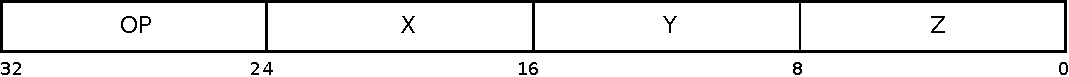
\includegraphics[width=\linewidth]{img/instruction-crop.pdf}

The first byte is the \i{opcode} of the instruction and the other three bytes specify the \i{operands}. Thus, MMIX allows (and uses) 256 instructions with 3 operands, each having 256 possible values. The typical instruction has the meaning "Set register {\tt X} to the result of {\tt Y} OP {\tt Z}". \citep[pg. 2]{mmix-doc}

In this thesis, all instructions are at first outlined with a box that contains the mnemonic, the operands of the instruction and the its effect. Afterwards the instruction is illustrated in further detail -- including special cases and raised \glslink{Exception}{AEs} or \glslink{Exception}{PEs}. The box looks like the following:
\instrtbl
	{\mi{ADD|SUB \$X,\$Y,\$Z|Z}}
	{$\dr{X} \leftarrow s(\dr{Y}) +|- \sdrimm{Z}$}

\noindent This describes the four instructions \mi{ADD}, \mi{ADDI}, \mi{SUB} and \mi{SUBI}. As in this example, many MMIX instructions come in two forms: In the first one, the {\tt Z}-operand is a register, in the second one it is an \glslink{Immediate Value}{immediate value}. Since there is no other difference, these are handled at once by saying "\udrim{Z}". Furthermore, \mi{ADD} and \mi{SUB} are very similar, so that they are grouped together. The notation $s(...)$ denotes, that MMIX interprets it as signed and uses two's complement arithmetic. Otherwise it means that MMIX treats the value as unsigned. Thus, the effect in the box shown above can be read as
\begin{itemize}
	\item \mi{ADD} sets \dr{X} to the result of the addition of \dr{Y} and \dr{Z}, interpreting both as signed values and hence, using signed arithmetic,
	\item \mi{ADDI} sets \dr{X} to the result of the addition of the signed value \dr{Y} and unsigned \glslink{Immediate Value}{immediate value} {\tt Z},
	\item \mi{SUB} sets \dr{X} to the result of the substraction of the signed value \dr{Y} and signed value \dr{Z} and
	\item \mi{SUBI} sets \dr{X} to the result of the substraction of the signed value \dr{Y} and unsigned \glslink{Immediate Value}{immediate value} {\tt Z}.
\end{itemize}
\glslink{Immediate Value}{Immediate values} are always interpreted unsigned in MMIX. Additionally, if one of the operands {\tt X}, {\tt Y} and {\tt Z} is not mentioned in the name, it means implicitly that the corresponding byte has to be zero. If it is not, MMIX will raise a \i{breaks rules} \glslink{Exception}{PE}.

Although the effects description will be straight forward for most of the instructions, it is not meant to be always complete or self-explaining, because that would be too verbose and would require a formal language definition for some instructions. Rather, it should be seen as a quick overview of what the instruction does. Thus, if necessary, the text below the box will clarify the effects description or adds further information.


\section{Registers}

Since the registers are one of the most important entities in MMIX, they are explained at first. MMIX has special, global and local registers, which will be described one after another in this section.

\subsection{Special Registers}

MMIX provides 32 special registers in an array called $sp$ in this thesis\footnote{The special registers may be put in the first 32 slots of the global register array, which is the reason why \sr{G} is always at least 32, as it will be mentioned in the next section. But actually, this is not enforced.}. Most of them will be introduced later as soon as the associated concept or instruction is described. The other ones, that don't fit into a certain category or are very important, are explained here.

\begin{itemize}
	\item \sr{A} - Arithmetic status register:\\
	Since \sr{A} affects many instructions, it is explained first. Its layout is:
	
	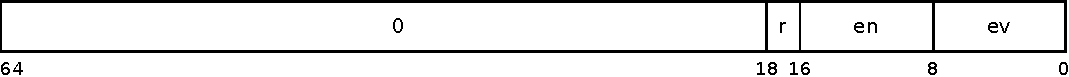
\includegraphics[width=\linewidth]{img/rA-crop.pdf}
	
	The fields $en$ and $ev$ contain \i{enable} and \i{event} bits, both called abbreviated "DVWIOUZX from left to right, where D stands for integer divide check, V for integer overflow, W for float-to-fix overflow, I for invalid operation, O for floating overflow, U for floating underflow, Z for floating division by zero, and X for floating inexact." \citep[pg. 26]{mmix-doc}
	The enable bits control whether an \glslink{Exception}{AE} is raised as soon as the corresponding exceptional condition occurs, while the event bits are set if no \glslink{Exception}{AE} has been raised.
	The field $r$ specifies the rounding mode that is used for floating point numbers, where $00_2$ means round near, $01_2$ round toward zero, $10_2$ round toward $+\infty$ and $11_2$ round toward $-\infty$. All other bits are defined to be zero. \citep[pg. 15 and 26]{mmix-doc}
	
	\item \sr{C} - Cycle counter:\\
	As the name suggests, MMIX increases this special register on every cycle by 1. It can be used to measure the performance of a code snippet, for example. \citep[pg. 32]{mmix-doc}
	\item \sr{I} - Interval counter:\\
	The special register \sr{I} is decreased by 1 on every cycle and causes an \i{interval \glslink{Interrupt}{interrupt}} as soon as it reaches zero. It can also be used for runtime analysis. \citep[pg. 32]{mmix-doc}
	\item \sr{U} - Usage counter:\\
	Register \sr{U} is structured in the following way:
	
	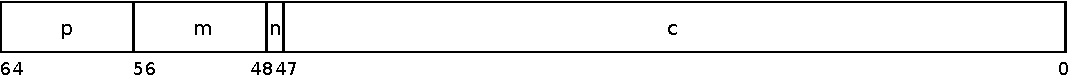
\includegraphics[width=\linewidth]{img/rU-crop.pdf}
	
	The usage count $c$ is increased whenever $OP \& m = p$, where $OP$ is the opcode of an instruction. The bit $n$ indicates whether it should also be done when the \glslink{PC}{instruction pointer} is in the privileged space. \citep[pg. 32]{mmix-doc}
	\item \sr{F} - Failure location register:\\
	This register holds the physical memory address when a parity error or other kinds of memory faults occur. Since an MMIX implementation may use caching, the instruction that caused this error might be long gone before it is detected. \citep[pg. 40]{mmix-doc}
	\item \sr{N} - Serial number:\\
	Register \sr{N} identifies the particular MMIX implementation and is structured as follows:
	
	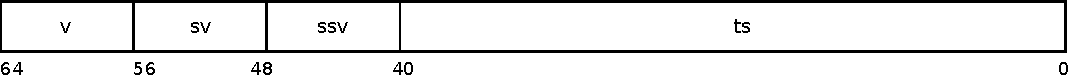
\includegraphics[width=\linewidth]{img/rN-crop.pdf}
	
	The fields $v$, $sv$ and $ssv$ specify the MMIX architecture version. This thesis describes version 1, subversion 0 and subsubversion 0, \ie 1.0.0. The field $ts$ holds the number of seconds from 01/01/1970, 00:00:00 GMT to the date the particular instance of MMIX was built on. \citep[pg. 32]{mmix-doc}
\end{itemize}

\noindent MMIX provides two instructions to read from or write to a special register.

\instrtbl
	{\mi{GET \$X,Z}}
	{\dr{X} $\leftarrow$ \spr{Z}}
\noindent The instruction \mi{GET} sets \dr{X} to the value of special register `Z`. MMIX doesn't keep secrets from the user, \ie all special registers are readable -- even in user mode. \citep[pg. 34]{mmix-doc}

\instrtbl
	{\mi{PUT X,\$Z|Z}}
	{\spr{X} $\leftarrow$ \udrim{Z}}
\noindent \mi{PUT} sets special register `X` to either \dr{Z} or the \glslink{Immediate Value}{immediate value} `Z`. The registers \sr{C}, \sr{N}, \sr{O} and \sr{S} are not writeable in general. \sr{I}, \sr{T}, \sr{TT}, \sr{K}, \sr{Q}, \sr{U} and \sr{V} are writeable in privileged mode only. Additionally, in \sr{A} all bits except \haddrt{3}{FFFF} have to be zero, \sr{G} can't be less than $max(\sr{L},32)$ and not greater than 255. Furthermore, \sr{L} can't be increased with \mi{PUT} and bits in the \i{\glslink{Interrupt}{interrupt} request register} \sr{Q}, that have been set by MMIX since the last execution of \mi{GET \dr{X},\sr{Q}}, can't be unset. In this way, no \glslink{Exception}{PE}, \glslink{Exception}{ME} or \glslink{Interrupt}{interrupt} bit can be lost by accident.\footnote{The restrictions will become more clear as soon as the concepts and instructions working with these registers have been explained.} \citep[pg. 34]{mmix-doc}

\subsection{Global and Local Registers}

MMIX maintains two banks of registers. One for global registers, called $g$, which has at most 256 slots. The other one for local registers, called $l$, which has $2^n$ slots, where $n$ is between 8 and 10. Both can be accessed by the so called \i{dynamic registers}, \dr{0}, \dr{1}, \dots, \dr{255}. MMIX uses the special register \sr{G} to separate them. \sr{G} is always at least 32 at at most 255. When saying \dr{X}, it denotes a global register whenever `X` is greater or equal to \sr{G}. It denotes a local register if it is less than \sr{G}. \citep[pg. 22]{mmix-doc}

Additionally, \sr{L} splits the local registers in two categories. The registers \dr{0}, \dots, \dr{(rL - 1)} are the local registers that are currently in use. The other ones, \dr{(rL)}, \dots, \dr{(rG - 1)}, are called \i{marginal}. If such a register is read, it always yields zero. If \dr{X} is written, where $\sr{L} \le {\tt X} < \sr{G}$, the registers \dr{(rL)}, \dots, \dr{(X - 1)} are set to zero, \dr{X} is set to the desired value and \sr{L} is set to ${\tt X} + 1$. \citep[pg. 22]{mmix-doc}

For example, if \sr{L} is 4 and \sr{G} is 64,
\begin{itemize}
	\item reading \dr{3} would yield the value of $l[3]$,
	\item reading \dr{4} would yield 0,
	\item writing 12 to \dr{5} would set $l[4]$ to 0, $l[5]$ to 12 and \sr{L} to 6,
	\item reading \dr{64} would yield the value of $g[64]$ and
	\item writing 100 to \dr{70} would set $g[70]$ to 100.
\end{itemize}


\section{Integer Arithmetic}

Of course, MMIX provides some instructions to perform integer arithmetic. That is, addition, substraction, multiplication, division and some more. For most of these instructions, MMIX has an unsigned and a signed version. The only difference when adding or substracting is, that the signed versions raise arithmetic \glslink{Exception}{exceptions} -- if necessary -- while the others won't. When multiplying or dividing, the rules for signed or unsigned arithmetic have to be considered.

\subsection{Addition and Substraction}

\instrtbl
	{\mi{ADD|SUB \$X,\$Y,\$Z|Z}}
	{$\dr{X} \leftarrow s(\dr{Y}) +|- \sdrimm{Z}$}
\noindent The sum or difference of \dr{Y} and \udrim{Z} is put into \dr{X}. An integer overflow \glslink{Exception}{AE} is raised if the result is $\ge 2^{63}$ or $< -2^{63}$. \citep[pg. 6]{mmix-doc}

\instrtbl
	{\mi{ADDU|SUBU \$X,\$Y,\$Z|Z}}
	{$\dr{X} \leftarrow (\dr{Y} +|- \udrim{Z}) \bmod 2^{64}$}
\noindent The sum or difference of \dr{Y} and \udrim{Z} is put into \dr{X}. \citep[pg. 6]{mmix-doc}

\instrtbl
	{\mi{NEG \$X,Y,\$Z|Z}}
	{$\dr{X} \leftarrow {\tt Y} - \sdrimm{Z}$}
\noindent MMIX provides a separate instruction for negation to save the programmer from having to put a constant into a register first. This way, \eg \dr{Z} can be negated by saying \mi{NEG \$X,0,\$Z}. It can also be used for building the value $-1$: \mi{NEG \$X,0,1}. The instruction throws an overflow \glslink{Exception}{AE} if the result is $> 2^{63}-1$. \citep[pg. 6]{mmix-doc}

\instrtbl
	{\mi{NEGU \$X,Y,\$Z|Z}}
	{$\dr{X} \leftarrow ({\tt Y} - \udrim{Z}) \bmod 2^{64}$}
\noindent This instruction has the same effect as \mi{NEG}, but does not raise an \glslink{Exception}{AE}. \citep[pg. 6]{mmix-doc}

\subsection{Multiplication and Division}

The more expensive integer arithmetic operations are multiplication and division. MMIX supports 64-bit signed multiplication and division and 128-bit unsigned multiplication and division. The division instructions perform a division and modulo calculation at once. Additionally it is worth noting that MMIX uses the so called \i{floored division}. This means that division rounds towards negative infinity and that the sign of the modulus is always the same as the sign of the divisor \citep[pg. 2]{divmod}. For example, this differs from the x86 architecture, which uses \i{truncated division} \citep[pg. 560]{ia32-sdmv2a}, that rounds towards zero and gives the modulus the sign of the dividend \citep[pg. 2]{divmod}. The following table illustrates the differences:

\begin{table}[h]
	\begin{tabular}{| >{\centering}p{20mm} | >{\centering}p{26mm} | >{\centering}p{26mm} | >{\centering}p{26mm} | >{\centering}p{26mm} |}
		\hline
		\textbf{Y,Z} &
		\textbf{$trunc(Y / Z)$} & \textbf{$trunc(Y \% Z)$} &
		\textbf{$\lfloor Y / Z \rfloor$} & \textbf{$\lfloor Y \% Z \rfloor$}
		\tabularnewline
		\hline
		$+8,+3$ & $+2$ & $+2$ & $+2$ & $+2$
		\tabularnewline
		\hline
		$+8,-3$ & $-2$ & $+2$ & $-3$ & $-1$
		\tabularnewline
		\hline
		$-8,+3$ & $-2$ & $-2$ & $-3$ & $+1$
		\tabularnewline
		\hline
		$-8,-3$ & $+2$ & $-2$ & $+2$ & $-2$
		\tabularnewline
		\hline
	\end{tabular}
	\caption{Comparison of truncated and floored division \citep[pg. 3]{divmod}}
\end{table}
\noindent The differences occur for numbers with different signs only, \ie the unsigned division does behave in the same way regardless of using the floored or truncated algorithm.

\instrtbl
	{\mi{MUL \$X,\$Y,\$Z|Z}}
	{$\dr{X} \leftarrow s(\dr{Y}) * \sdrimm{Z}$}
\noindent The \mi{MUL} instruction sets \dr{X} to the result of the multiplication. It raises an integer overflow \glslink{Exception}{AE} if the result is $\ge 2^{63}$ or $< -2^{63}$. \citep[pg. 14]{mmix-doc}

\instrtbl
	{\mi{MULU \$X,\$Y,\$Z|Z}}
	{$\dr{X} \leftarrow (\dr{Y} * \udrim{Z}) \bmod 2^{64},\quad
	\sr{H} \leftarrow (\dr{Y} * \udrim{Z}) \gg 64$}
\noindent This instruction basically does the same as \mi{MUL}, but treats the operands as unsigned and places the upper 64 bit of the result into the special \i{himult register} \sr{H} and does not raise an overflow \glslink{Exception}{AE}. \citep[pg. 14]{mmix-doc}

\instrtbl
	{\mi{DIV \$X,\$Y,\$Z|Z}}
	{$\dr{X} \leftarrow \lfloor s(\dr{Y})~/~\sdrimm{Z}\rfloor,\quad
	\sr{R} \leftarrow s(\dr{Y}) \bmod \sdrimm{Z}$}
\noindent The instruction \mi{DIV} sets \dr{X} to the result of the division and the \i{remainder register} \sr{R} to the result of the modulo operation. If \sdrim{Z} is zero, a division by zero \glslink{Exception}{AE} is raised, \dr{X} is set to zero and \sr{R} is set to \dr{Y}. An integer overflow \glslink{Exception}{AE} occurs if and only if $-2^{63}$ is divided by $-1$. \citep[pg. 14]{mmix-doc}

\instrtbl
	{\mi{DIVU \$X,\$Y,\$Z|Z}}
	{$\dr{X} \leftarrow \lfloor \sr{D}\dr{Y}~/~\udrim{Z}\rfloor,\quad
	\sr{R} \leftarrow \sr{D}\dr{Y} \bmod \udrim{Z}$}
\noindent Analogous to \mi{MULU}, \mi{DIVU} prefixes the \i{dividend register} \sr{D} to \dr{Y}, resulting in a 128-bit number, and divides it by \udrim{Z}, using unsigned arithmetic. If $\sr{D} \ge \udrim{Z}$ (this includes the case that \udrim{Z} is zero), \dr{X} is set to \sr{D} and \sr{R} is set to \dr{Y}. Additionally, no \glslink{Exception}{AE} is raised. \citep[pg. 14]{mmix-doc}

\medskip

\instrtbl
	{\mi{2ADDU|4ADDU|8ADDU|16ADDU \$X,\$Y,\$Z|Z}}
	{$\dr{X} \leftarrow ((2|4|8|16 * \dr{Y}) + \udrim{Z}) \bmod 2^{64}$}
\noindent As usual, if a number should be divided or multiplied by a power of 2, shifts are much more efficient, which will be described later. MMIX goes even further by providing instructions that multiply a number by 2, 4, 8 or 16 and adding the result to another value. In this way, one can easily e.g. multiply by 3 by saying \mi{2ADDU \$X,\$Y,\$Y}. \citep[pg. 6]{mmix-doc}


\section{Bit Fiddling}

MMIX has quite a few instructions for manipulating bits. At first, the well known bit operations {\tt AND}, {\tt OR}, {\tt NOR}, \dots and shifts are described, because they won't be a surprise.

\subsection{Basic Bit Operations}

\instrtbl
	{\mi{AND|OR|XOR|ANDN|ORN|NAND|NOR|NXOR \$X,\$Y,\$Z|Z}}
	{$\dr{X} \leftarrow \dr{Y} \land|\lor|\oplus|\land \sim|\lor \sim|\mathbin{\overline\land}|\mathbin{\overline\lor}|\mathbin{\overline\oplus} \udrim{Z}$}
\noindent These instructions set \dr{X} to the result of the corresponding bit operation with operands \dr{Y} and \udrim{Z}. The instructions that end with '\mi{N}' logically negate \udrim{Z} first and apply the operation without '\mi{N}' (\mi{OR} or \mi{AND}) afterwards. \citep[pg. 7]{mmix-doc}

\instrtbl
	{\mi{SL|SLU|SR|SRU \$X,\$Y,\$Z|Z}}
	{$\dr{X} \leftarrow \dr{Y} \ll|\ll|\gg|\ggg \udrim{Z}$}
\noindent The instructions for shifting left, \mi{SL} and \mi{SLU}, have the same behaviour, except that \mi{SL} will raise an integer overflow \glslink{Exception}{AE}, if the result is $\ge 2^{63}$ or $< -2^{63}$. \mi{SR} performs an arithmetic right shift, \ie it shifts in copies of the sign bit from the left, and \mi{SRU} performs a logical right shift, \ie it shifts in zeros from the left. Since \udrim{Z} is treaten unsigned, one can't use \mi{SL} to shift right or similar. Additionally it is worth mentioning, that a logical shift left or right of 64 or more will set \dr{X} to zero, whereas an arithmetical shift right of 64 or more will set \dr{X} to $-1$, if \dr{Y} is negative and to zero otherwise. \citep[pg. 10]{mmix-doc}

\subsection{Wyde Operations}

If one liked to put an arbitrary 64-bit constant into a register or manipulate individual wydes of a registers, one could use one of the following 16 instructions.

\instrtbl
	{\mi{SETH|SETMH|SETML|SETL \$X,YZ}}
	{$\dr{X} \leftarrow {\tt YZ} \ll 48|32|16|0$}
\noindent These instructions set the corresponding wyde of \dr{X} to the 16-bit constant {\tt YZ} and all other wydes to zero \citep[pg. 7]{mmix-doc}. That means, for example \mi{SETMH \$X,\haddr{1234}} sets \dr{X} to \haddro{0000}{1234}{0000}{0000}.

\instrtbl
	{\mi{ORH|ORMH|ORML|ORL \$X,YZ}}
	{$\dr{X} \leftarrow \dr{X} \lor ({\tt YZ} \ll 48|32|16|0)$}
\noindent Similarly, these instructions {\tt OR} the 16-bit constant {\tt YZ} into the corresponding wyde of \dr{X} \citep[pg. 7]{mmix-doc}. For example, if \dr{X} is \haddro{0000}{F0F0}{FF00}{0000}, a \mi{ORML \$X,\haddr{0FF0}} will result in \haddro{0000}{F0F0}{FFF0}{0000}.

\instrtbl
	{\mi{ANDNH|ANDNMH|ANDNML|ANDNL \$X,YZ}}
	{$\dr{X} \leftarrow \dr{X}~\land \sim({\tt YZ} \ll 48|32|16|0)$}
\noindent Analogous to the {\tt ORX} family, these instructions remove the bits set in the 16-bit constant {\tt YZ} from the corresponding wyde of \dr{X} \citep[pg. 7]{mmix-doc}. For example, if \dr{X} is \haddro{0000}{F0F0}{FF00}{0000}, a \mi{ANDNML \$X,\haddr{F000}} will result in \haddro{0000}{F0F0}{0F00}{0000}.

\instrtbl
	{\mi{INCH|INCMH|INCML|INCL \$X,YZ}}
	{$\dr{X} \leftarrow (\dr{X} + ({\tt YZ} \ll 48|32|16|0)) \bmod 2^{64}$}
\noindent Last but not least, the {\tt INCX} family adds the 16-bit constant {\tt YZ} to the corresponding wyde of \dr{X}, ignoring overflow \citep[pg. 7]{mmix-doc}. For example, if \dr{X} is \haddro{0000}{F0F0}{FF00}{0000}, an \mi{INCML \$X,\haddr{0101}} will result in \haddro{0000}{F0F1}{0001}{0000} (as shown with the example, other wyde may be affected as well, in contrast to the other wyde instructions).

\subsection{Exotic Bit Operations}

Apart from the simple bit operations just described, MMIX does also support more exotic ones that probably will not be used very often, but allow to do complicated computations in hardware instead of in software, as it would be necessary with other architectures.

\instrtbl
	{\mi{MUX \$X,\$Y,\$Z|Z}}
	{$\dr{X} \leftarrow (\dr{Y} \land \sr{M}) \lor (\udrim{Z} \land \mathbin{\overline{\sr{M}}})$}
\noindent The first rather exotic operation is the \i{bitwise multiplexer} \mi{MUX}. For each bit position $i$, it sets bit $\dr{Y}_i$, if $\sr{M}_i$ is 1, and bit $\udrim{Z_i}$, if $\sr{M}_i$ is 0 \citep[pg. 7]{mmix-doc}. For example, if \sr{M} is \haddro{FFFF}{0000}{FFFF}{0000}, \dr{0} is \haddro{1234}{5678}{90AB}{CDEF} and \dr{1} is \haddro{FFFF}{FFFF}{FFFF}{FFFF}, a \mi{MUX \$X,\$0,\$1} will set \dr{X} to \haddro{1234}{FFFF}{90AB}{FFFF}.

\instrtbl
	{\mi{BDIF|WDIF|TDIF|ODIF \$X,\$Y,\$Z|Z}}
	{$\dr{X}_i \leftarrow max(0,\dr{Y}_i - \udrim{Z_i})$ for each byte|wyde|tetra|octa $i$}
\noindent The second family in this category is the byte, wyde, tetra and octa difference. For example, \mi{BDIF} takes the byte $i$ of \dr{Y}, namely $\dr{Y}_i$, and substracts the byte $\udrim{Z_i}$ from it. If the difference is less than zero, $\dr{X}_i$ is set to zero. Otherwise it is set to the difference. This is done individually for every byte pair. \mi{WDIF}, \mi{TDIF} and \mi{ODIF} behave analogous using wydes, tetras and octas, respectively. These instructions are for example useful, when a graphical application wants to calculate the "pixel difference", \ie the absolute difference of colors, each color component represented as a byte. \citep[pg. 8]{mmix-doc}

\instrtbl
	{\mi{SADD \$X,\$Y,\$Z|Z}}
	{$\dr{X} \leftarrow countbits(\dr{Y} \setminus \udrim{Z})$}
\noindent The \i{sideways addition} \mi{SADD} performs at first the complement of \udrim{Z} and logically ands the result with \dr{Y}. Afterwards the number of set bits in this value is put into \dr{X}. \citep[pg. 9]{mmix-doc} So, for example, if \dr{0} is \haddr{8642} and \dr{1} is \haddr{8002}, a \mi{SADD \$X,\$0,\$1} will put 3 into \dr{X}. Because the difference, \haddr{0640}, has 3 bits set.

\instrtbl
	{\mi{MOR|MXOR \$X,\$Y,\$Z|Z}}
	{$\dr{X} \leftarrow mat(\dr{Y}) \lor|\oplus mat(\udrim{Z})$}
\noindent The last exotic bit operation, called \i{multiple or/exclusive-or}, is the most complicated one. It treats \dr{Y} and \udrim{Z} as $8 \times 8$ bit matrices, using one byte for each column, and performs a kind of matrix product using \mi{OR} or \mi{XOR} instead of the multiplication. More precisely, when the bits of \dr{Y} and \udrim{Z} are numbered as
$$y_{00}y_{01}\ldots y_{07}y_{10}y_{11}\ldots y_{17}\ldots y_{70}y_{71}\ldots y_{77}\quad
z_{00}z_{01}\ldots z_{07}z_{10}z_{11}\ldots z_{17}\ldots z_{70}z_{71}\ldots z_{77},$$
each bit $x_{ij}$ of \dr{X} is set to
$$(y_{0j}\land z_{i0})\lor (y_{1j}\land z_{i1})\lor \cdots \lor (y_{7j}\land z_{i7}).$$
When using \mi{MXOR} instead of \mi{MOR}, the {\tt OR}s are replaced by {\tt XOR}s. \mi{MOR} can be used for example to convert between big endian and little endian. \citep[pg. 9]{mmix-doc} If \dr{0} is \haddro{0123}{4567}{89AB}{CDEF} and \dr{1} is \haddro{0102}{0408}{1020}{4080}, a \mi{MOR \$X,\$0,\$1} will perform the following operation:
\[
\left(%
\begin{array}{*{8}{>{\centering\arraybackslash$}p{1mm}<{$}}}
	0 & 0 & 0 & 0 & 1 & 1 & 1 & 1 \\
	\rowcolor{lightgray}0 & 0 & 1 & 1 & 0 & 0 & 1 & 1 \\
	0 & 1 & 0 & 1 & 0 & 1 & 0 & 1 \\
	0 & 0 & 0 & 0 & 0 & 0 & 0 & 0 \\
	0 & 0 & 0 & 0 & 1 & 1 & 1 & 1 \\
	0 & 0 & 1 & 1 & 0 & 0 & 1 & 1 \\
	0 & 1 & 0 & 1 & 0 & 1 & 0 & 1 \\
	1 & 1 & 1 & 1 & 1 & 1 & 1 & 1
\end{array}
\right)
\lor
\left(%
\begin{array}{*{8}{>{\centering\arraybackslash$}p{1mm}<{$}}}
	0 & 0 & 0 & \cellcolor{lightgray}0 & 0 & 0 & 0 & 1 \\
	0 & 0 & 0 & \cellcolor{lightgray}0 & 0 & 0 & 1 & 0 \\
	0 & 0 & 0 & \cellcolor{lightgray}0 & 0 & 1 & 0 & 0 \\
	0 & 0 & 0 & \cellcolor{lightgray}0 & 1 & 0 & 0 & 0 \\
	0 & 0 & 0 & \cellcolor{lightgray}1 & 0 & 0 & 0 & 0 \\
	0 & 0 & 1 & \cellcolor{lightgray}0 & 0 & 0 & 0 & 0 \\
	0 & 1 & 0 & \cellcolor{lightgray}0 & 0 & 0 & 0 & 0 \\
	1 & 0 & 0 & \cellcolor{lightgray}0 & 0 & 0 & 0 & 0
\end{array}
\right)
=
\left(%
\begin{array}{*{8}{>{\centering\arraybackslash$}p{1mm}<{$}}}
	1 & 1 & 1 & 1 & 0 & 0 & 0 & 0 \\
	1 & 1 & 0 & \cellcolor{lightgray}0 & 1 & 1 & 0 & 0 \\
	1 & 0 & 1 & 0 & 1 & 0 & 1 & 0 \\
	0 & 0 & 0 & 0 & 0 & 0 & 0 & 0 \\
	1 & 1 & 1 & 1 & 0 & 0 & 0 & 0 \\
	1 & 1 & 0 & 0 & 1 & 1 & 0 & 0 \\
	1 & 0 & 1 & 0 & 1 & 0 & 1 & 0 \\
	1 & 1 & 1 & 1 & 1 & 1 & 1 & 1
\end{array}
\right)
\]
Analogous to the matrix product, the highlighted cell in the result matrix is built by {\tt AND}ing each cell in the highlighted row of \dr{Y} with the corresponding highlighted cell of \udrim{Z} individually, starting on the left and top, respectively, and performing an {\tt OR} of all these values. In this case, there is no pair of bits in which both are 1 and thus, the highlighted cell in the result is 0. Doing that for all cells leads to the value \haddro{EFCD}{AB89}{6745}{2301}, \ie the bytes of \dr{0} in the opposite order. \citep[pg. 192]{mmix-buch}


\section{Comparisons}

MMIX has four instructions to compare numbers, which for example can be used for branching. Additionally, it has instructions to conditionally set and zero or set a register.

\instrtbl
	{\mi{CMP \$X,\$Y,\$Z|Z}}
	{$\dr{X} \leftarrow (s(\dr{Y}) > \sdrimm{Z}) - (s(\dr{Y}) < \sdrimm{Z})$}
\noindent The instruction \mi{CMP} compares \dr{Y} with \udrim{Z} using signed arithmetic and puts the result into \dr{X}. If \dr{Y} is less than \udrim{Z}, \dr{X} is set to $-1$, if they are equal, \dr{X} is set to 0 and if \dr{Y} is greater than \udrim{Z}, \dr{X} is set to 1. \citep[pg. 11]{mmix-doc}

\instrtbl
	{\mi{CMPU \$X,\$Y,\$Z|Z}}
	{$\dr{X} \leftarrow (\dr{Y} > \udrim{Z}) - (\dr{Y} < \udrim{Z})$}
\noindent This instruction behaves like \mi{CMPU}, but uses unsigned arithmetic. \citep[pg. 11]{mmix-doc}

\instrtbl
	{\mi{CSN|CSZ|CSP|CSOD|CSNN|CSNZ|CSNP|CSEV \$X,\$Y,\$Z|Z}}
	{if $s(\dr{Y}) <0|=0|>0|odd|\ge0|\ne0|\le0|even$: $\dr{X} \leftarrow \udrim{Z}$}
\noindent The family of conditional set instructions sets \dr{X} to \udrim{Z}, if \dr{Y} is negative, zero, positive, odd, nonnegative, nonzero, nonpositive or even. Otherwise nothing happens. \citep[pg. 11]{mmix-doc}

\instrtbl
	{\mi{ZSN|ZSZ|ZSP|ZSOD|ZSNN|ZSNZ|ZSNP|ZSEV \$X,\$Y,\$Z|Z}}
	{$\dr{X} \leftarrow (s(\dr{Y}) <0|=0|>0|odd|\ge0|\ne0|\le0|even)~?~\udrim{Z}~:~0$}
\noindent Very similar to the conditional set instructions, the zero or set instructions set \dr{X} either to \udrim{Z} or zero, depending on whether \dr{Y} is negative, zero, positive, odd, nonnegative, nonzero, nonpositive or even. \citep[pg. 11]{mmix-doc}

\medskip

MMIX does also provide an atomic \i{compare and swap} instruction. It can be used for interprocess communication with shared memory or to synchronize threads in the same process. Since MMIX is not only designed to work on a single processor, this instruction might also be helpful when independent computers are sharing the same memory. \citep[pg. 25]{mmix-doc}

\instrtblfour
	{\mi{CSWAP \$X,\$Y,\$Z|Z}}
	{if $\vmem{8}{\dr{Y} + \udrim{Z}}~= \sr{P}$:}
	{$\quad \vmem{8}{\dr{Y} + \udrim{Z}}~\leftarrow \dr{X},\quad \dr{X} \leftarrow 1$}
	{else:}
	{$\quad \sr{P} \leftarrow \vmem{8}{\dr{Y} + \udrim{Z}},\quad \dr{X} \leftarrow 0$}
\noindent The \i{compare and swap octabytes} instruction compares \vmem{8}{\dr{Y} + \udrim{Z}} with the special \i{prediction register} \sr{P} and either replaces the octa in memory with \dr{X} or \sr{P} with the octa in memory, depending on whether \sr{P} is equal to the octa. \dr{X} indicates whether the octa in memory has been replaced. \citep[pg. 25]{mmix-doc} For example, one could set \dr{0} to 1, \sr{P} to 0 and do a \mi{CSWAP \$0,\$Y,\$Z|Z}, assuming that $\dr{Y} + \udrim{Z}$ denotes the memory location that is desired for synchronization. If \dr{0} has been set to 1, the lock has been aquired successfully. If not, the whole procedure is repeated. That means, \vmem{8}{\dr{Y} + \udrim{Z}} being 1 or 0 would indicate that someone currently has the lock or not, respectively.


\section{Branches and Jumps}

Of course, MMIX does also need instructions to change the course of computation. To allow programs to use a pipeline implementation of MMIX in an efficient way, it provides both ordinary branches and probable branches. For consistency, the different kinds of comparisons offered by branches are the same as those existing for the conditional set and zero or set instructions.

Similarly to the fact, that the typical "set register {\tt X} to the result of {\tt Y} OP {\tt Z}" instructions come in two versions -- one with {\tt Z} as a register, one with {\tt Z} as an \glslink{Immediate Value}{immediate value} -- the branch and jump instructions also come in two versions. The first one branches or jumps forward, while the second one branches or jumps backwards. The backward versions are suffixed with a '{\tt B}'.

\instrtbl
	{\mi{BN|BZ|BP|BOD|BNN|BNZ|BNP|BEV \$X,@+4*(YZ[-$2^{16}$])}}
	{if $s(\dr{X}) <0|=0|>0|odd|\ge0|\ne0|\le0|even$: $@ \leftarrow @+4*({\tt YZ}[-2^{16}])$}
\noindent If \dr{X} is negative, zero, positive, odd, nonnegative, nonzero, nonpositive or even, the branch will be taken. The forward versions increase the \glslink{PC}{instruction pointer} by $4*{\tt YZ}$, \ie the value of the unsigned 16-bit \glslink{Immediate Value}{immediate value} {\tt YZ} multiplied with the number of bytes of an instruction. The backward versions increase it by $4*({\tt YZ}-2^{16})$. Thus, these instructions allow to change $@$ to any instruction in $(@ - 4*2^{16}) \dots (@ + 4*(2^{16}-1))$. It should be noted, that this category of branches tell MMIX that the branch will probably not be taken. This may affect the runtime on some implementations of MMIX. \citep[pg. 12]{mmix-doc}

\instrtbl
	{\mi{PBN|PBZ|PBP|PBOD|PBNN|PBNZ|PBNP|PBEV \$X,@+4*(YZ[-$2^{16}$])}}
	{if $s(\dr{X}) <0|=0|>0|odd|\ge0|\ne0|\le0|even$: $@ \leftarrow @+4*({\tt YZ}[-2^{16}])$}
\noindent These instructions behave exactly in the same way as the previously introduced ones. The only difference is, that these tell MMIX that the branch will probably be taken. \citep[pg. 12]{mmix-doc}

\instrtbl
	{\mi{JMP @+4*(XYZ[-$2^{24}$])}}
	{$@ \leftarrow @+4*({\tt XYZ}[-2^{24}])$}
\noindent Of course, MMIX has also an instruction to change the \glslink{PC}{instruction pointer} unconditionally: the jump. It simply sets $@$ to $(@+4*({\tt XYZ}[-2^{24}]))$, \ie the forward version increases $@$ by the unsigned 24-bit constant {\tt XYZ}, multiplied by 4. The backward version substracts $2^{24}$ from {\tt XYZ} before multiplying. Thus, one can jump to any instruction in the range $(@ - 4*2^{24}) \dots (@ + 4*(2^{24}-1))$. \citep[pg. 13]{mmix-doc}

\instrtbl
	{\mi{GO \$X,\$Y,\$Z|Z}}
	{$\dr{X} \leftarrow @+4,\quad @ \leftarrow \dr{Y} + \udrim{Z}$}
\noindent To be able to jump to any location in the virtual address space, MMIX has the instruction \mi{GO}. It simply changes the \glslink{PC}{instruction pointer} to $\dr{Y} + \udrim{Z}$. Additionally, \dr{X} is set to the location that ordinary would have been executed next. That allows using \mi{GO} for a simple type of \glslink{Subroutine linkage}{subroutine linkage} by not overwriting \dr{X} in the subroutine and returning via \mi{GO \$X,\$X,0}. But MMIX provides another mechanism, that is much better suited for that task, because it makes subroutines independent of each other, as will be described later in this chapter. An interesting corner case is, that \mi{GO} permits it to jump to addresses that are not tetra-aligned. MMIX will simply set the desired \glslink{PC}{instruction pointer}, but this is not going to be a problem because when loading \vmem{4}{@}, the least significant 2 bits of $@$ are ignored. \citep[pg. 13]{mmix-doc}

\instrtbl
	{\mi{GETA \$X,@+4*(YZ[-$2^{16}$])}}
	{$\dr{X} \leftarrow @+4*({\tt YZ}[-2^{16}])$}
\noindent This instruction does not change the \glslink{PC}{instruction pointer}, but is related because it builds an absolute address from the \glslink{PC}{instruction pointer} and the {\tt YZ} field. \mi{GETA} comes in two versions for forward and backwards calculations and uses the same rules for that as the branches do. \citep[pg. 13]{mmix-doc}


\section{Memory}

The memory hierarchy is one of the more complicated concepts in MMIX. This section starts by explaining the load and store instructions, which are rather simple. Afterwards the structure of the virtual and physical address space is described, followed by the translation mechanism and the translation caches. Finally, the instructions interesting for physical memory caches, which may be present in a particular implementation of MMIX, are introduced.

\subsection{Load Instructions}

MMIX has two kinds of load instructions for each quantity: a signed version and an unsigned version. The difference is that the signed versions treat the number in memory as signed and thus sign-extend the value to 64 bit.

\instrtbl
	{\mi{LDB|LDW|LDT|LDO \$X,\$Y,\$Z|Z}}
	{$\dr{X} \leftarrow s(\vmem{1|2|4|8}{\dr{Y} + \udrim{Z}})$}
\noindent These are the signed load instructions, which set \dr{X} to the byte, wyde, tetra or octa at the specified location in memory. \mi{LDB}, \mi{LDW} and \mi{LDT} will sign-extend the number, \ie the bits in the upper 7, 6 and 4 bytes, respectively, are set to copies of the sign-bit of the number in memory. \citep[pg. 4]{mmix-doc}

\instrtbl
	{\mi{LDBU|LDWU|LDTU|LDOU \$X,\$Y,\$Z|Z}}
	{$\dr{X} \leftarrow $~\vmem{1|2|4|8}{\dr{Y} + \udrim{Z}}}
\noindent As already mentioned, the unsigned versions have the same behaviour, except that they do not sign-extend the values. \mi{LDOU} and \mi{LDO} are completely identical and only exist both for consistency. \citep[pg. 4]{mmix-doc}

\instrtbl
	{\mi{LDHT \$X,\$Y,\$Z|Z}}
	{$\dr{X} \leftarrow~\vmem{4}{\dr{Y} + \udrim{Z}}~\ll 32$}
\noindent The last load instruction, \i{load high tetra}, puts the tetra \vmem{4}{\dr{Y} + \udrim{Z}} into the higher half or \dr{X}. The other half is cleared to zero. \citep[pg. 4]{mmix-doc}

\subsection{Store Instructions}

Analogous to the load instructions, MMIX provides two store instructions for every quantity. In this case, the signed versions throw an integer overflow \glslink{Exception}{AE}, if the number can not be represented with the corresponding quantity, while the unsigned versions do not.

\instrtbl
	{\mi{STB|STW|STT|STO \$X,\$Y,\$Z|Z}}
	{$\vmem{1|2|4|8}{\dr{Y} + \udrim{Z}}~\leftarrow s(\dr{X})$}
\noindent These instructions write the signed number in \dr{X} to the corresponding location in memory. \mi{STB} will throw an integer overflow \glslink{Exception}{AE}, if \dr{X} is not between $-128$ and $+127$, \mi{STW} if \dr{X} is not between $-32,768$ and $+32,767$ and \mi{STT} if \dr{X} is not between $-2,147,483,648$ and $+2,147,483,647$. \mi{STO} will not throw an integer overflow \glslink{Exception}{AE}. \citep[pg. 5]{mmix-doc}

\instrtbl
	{\mi{STBU|STWU|STTU|STOU \$X,\$Y,\$Z|Z}}
	{$\vmem{1|2|4|8}{\dr{Y} + \udrim{Z}}~\leftarrow \dr{X}$}
\noindent The unsigned store instructions are the same as their signed correspondence, but do not test for overflow. \citep[pg. 5]{mmix-doc}

\instrtbl
	{\mi{STHT \$X,\$Y,\$Z|Z}}
	{$\vmem{4}{\dr{Y} + \udrim{Z}}~\leftarrow \dr{X} \gg 32$}
\noindent Similarly to load high tetra, \i{store high tetra} stores the most significant four bytes of \dr{X} to \vmem{4}{\dr{Y} + \udrim{Z}}. \citep[pg. 5]{mmix-doc}

\instrtbl
	{\mi{STCO X,\$Y,\$Z|Z}}
	{$\vmem{8}{\dr{Y} + \udrim{Z}}~\leftarrow {\tt X}$}
\noindent For convenience and efficiency, MMIX provides another store instruction, \i{store constant octabyte}, which stores the unsigned \glslink{Immediate Value}{immediate value} {\tt X} as an octa to the desired location in memory. This saves the programmer from having to put the constant into a register first. \citep[pg. 5]{mmix-doc}

\subsection{Virtual and Physical Address Space}

As already mentioned at the beginning, MMIX has both a 64-bit virtual and physical address space. Their layout is illustrated by the following figure:
\begin{figure}[H]
	\centering
	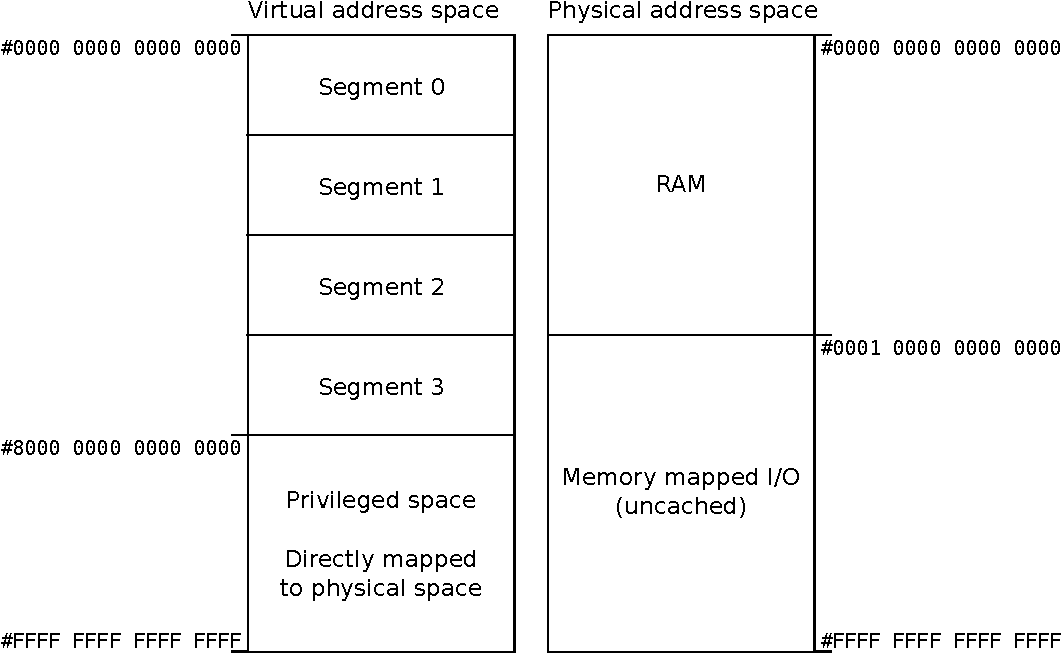
\includegraphics[width=\textwidth]{img/address-spaces-crop.pdf}
	\caption{Virtual and physical address space layout \citep[pg. 35]{mmix-doc}}
\end{figure}
\noindent The virtual address space is divided in user space and privileged space. The privileged space is directly mapped to the physical address space, called m. That means, \vmem{}{{\tt X}}$~=~$m[${\tt X}~\land~$\haddro{7FFF}{FFFF}{FFFF}{FFFF}$]$, if ${\tt X} \ge 2^{63}$. The user space is divided into four segments, determined by the most significant 3 bits using $000_2$, $001_2$, $010_2$ and $011_2$ for segment 0, 1, 2 and 3, respectively. The use of these segments is not restricted by the hardware, but each segment is translated separately, as will be described in the next section.

The first 256 terabyte of the physical space are used for RAM. The remaining space is reserved for I/O devices. The layout of the I/O space is implementation dependent, but MMIX defines that the I/O space is always uncached, regardless of whether the particular MMIX implementation uses caching or not. \citep[pg. 35]{mmix-doc}

\subsubsection{Address Translation}

Besides the privileged space, which is directly mapped to the physical space, the user space is translated to the physical one via a quite complicated scheme. This section describes how this translation works in detail.

\paragraph{The Virtual Translation Register}

The translation is defined by register \sr{V}, which has the following layout:
\begin{figure}[H]
	\centering
	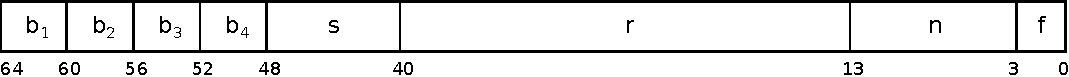
\includegraphics[width=\textwidth]{img/rV-crop.pdf}
\end{figure}
\vspace{-20pt}
\noindent The first two bytes of \sr{V} specify the number of pages in the four segments. Segment $i$ has at most $1024^{b_{i+1}-b_i}$ pages, where $b_0$ is defined to be zero. If $b_i = b_{i+1}$, segment $i$ must have at most one page and if $b_i > b_{i+1}$, segment i must be empty. For example,
\begin{itemize}
	\item if $b_1 = 1$, $b_2 = 2$, $b_3 = 3$ and $b_4 = 4$, all segments have at most 1024 pages,
	\item if $b_1 = 3$, $b_2 = 2$, $b_3 = 1$ and $b_4 = 0$, segment 0 has at most $1024^3$ pages and all other segments are empty and
	\item if $b_1 = 1$, $b_2 = 0$, $b_3 = 0$ and $b_4 = 0$, segment 0 has at most 1024 pages, segment 1 is empty and segments 2 and 3 have both at most 1 page.
\end{itemize}
The next field, called $s$, specifies that the page size is $2^s$, where $s$ has to be at least 13 and at most 48. The field $r$ tells MMIX the \i{root location}, which will be described in further detail shortly. The field $n$ holds the \i{address space number} and last but not least, $f$ is the \i{function field}, which specifies whether virtual address translation will be done by software ($f=1$) or by hardware ($f=0$). Other values are illegal. If translation by software is requested, MMIX ignores $b_1$, $b_2$, $b_3$, $b_4$ and $r$ of \sr{V} and lets the software decide how the actual translation mechanism works. That means, the following structures and concepts only apply if hardware translation is used. \citep[pg. 36]{mmix-doc}

\paragraph{The Root Location}

The field $r$ specifies an area in memory that holds the \glslink{Paging}{paging} structures for the current virtual address space. For each segment $i$ it holds $b_{i+1} - b_i$ page tables with either \i{page table entries} (PTEs) or \i{page table pointers} (PTPs), which are described in the next paragraphs. The page tables in the root location are, one could say, the "first layer" of the translation, because PTPs point to other page tables that reside in a different location in memory.

\paragraph{Page Table Entries}

A PTE defines to which page in physical memory a page in virtual memory is mapped to. Additionally it specifies the access permissions for that page. A PTE looks like the following:
\begin{figure}[H]
	\centering
	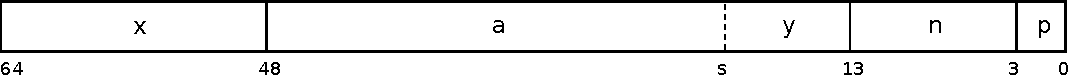
\includegraphics[width=\textwidth]{img/PTE-crop.pdf}
\end{figure}
\vspace{-20pt}
\noindent The field $a$ holds the physical address divided by the page size, \ie the physical address is $a * 2^s$. The field $n$ is the address space number, which has to be equal to $n$ in \sr{V}. The access permissions are defined by $p$ with bit 0 for executing, bit 1 for writing and bit 2 for reading. That means, for example $p=101_2$ makes the page readable and executable. The fields $x$ and $y$ are ignored by the hardware, which allows the operating system to use them for any purpose. \citep[pg. 36]{mmix-doc} It is noteworthy, that $y$ would be empty, if the page size were $2^{13}$, and $a$ would be empty, if the page size were $2^{48}$. Additionally, the layout of a PTE clarifies the reason for the page size restrictions.

\paragraph{Page Table Pointers}

PTPs are pointers to other page tables that may either hold PTPs as well or hold PTEs. They have the following layout:
\begin{figure}[H]
	\centering
	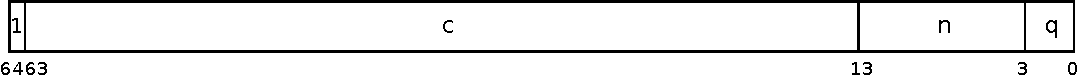
\includegraphics[width=\textwidth]{img/PTP-crop.pdf}
\end{figure}
\vspace{-20pt}
\noindent Similarly to the field $a$ of a PTE, the field $c$ of a PTP specifies the address of the page table this PTP links to, divided by the page size. The field $n$ has to match $n$ in \sr{V} as well, while $q$ is ignored and the most significant bit has to be 1. This forces the operating system to put a privileged address into a PTP, which is -- as already mentioned -- directly mapped. \citep[pg. 36]{mmix-doc}

\paragraph{The Translation Process}

Finally, the actual translation process should be described. If address $A$ should be translated, the segment is determined by $i = \lfloor A / 2^{61} \rfloor$. The page number in this segment is $A_p = \lfloor (A~\land~$\haddro{1FFF}{FFFF}{FFFF}{FFFF}$) / 2^s \rfloor$. Assuming that $A_p$ is equal to $(a_4a_3a_2a_1a_0)_{1024}$ (in the number system with base 1024), the translation works as follows:
\begin{itemize}
	\item if $a_4=a_3=a_2=a_1=0$, the PTE $e$ is \pmem{8}{2^{13}(r + b_i) + 8a_0} and thus, \vmem{}{A} corresponds to \pmem{}{2^s*e.a + (A \bmod 2^s)}.
	\item if $a_4=a_3=a_2=0$, the auxiliary PTP $p$ is used first, \ie \pmem{8}{2^{13}(r + b_i + 1)+8a_1}. In this case, the PTE is \pmem{8}{2^{13}*p.c + 8a_0}. Thus, one level of indirection is used.
	\item if $a_4=a_3=0$, two levels of indirection are used. That means, the first PTP $p1$ is \pmem{8}{2^{13}(r + b_i + 2)+8a_2} and determines the next PTP. This one, $p2$, is \pmem{8}{2^{13}*p1.c + 8a_1}. And finally the PTE is \pmem{8}{2^{13}*p2.c + 8a_0}.
	\item \dots
\end{itemize}
\citep[pg. 36]{mmix-doc} It is noteworthy, that when using the minimum page size of $2^{13}$, four levels of indirection are sufficient to cover a whole segment. Because $2^{13} * 1024 * 1024^4 = 2^{63}$ covers even more than one segment. Additionally, it is worth mentioning that the first slot in PTP page tables in the root location is actually never used. Because this slot is covered by the previous page table in the root location.

\paragraph{Example}

To clarify the just explained concepts and to show the layout in memory, which they imply, the following goes through an example. Supposed that \sr{V} and the \glslink{Paging}{paging} structures in memory are filled as:
\begin{figure}[H]
	\centering
	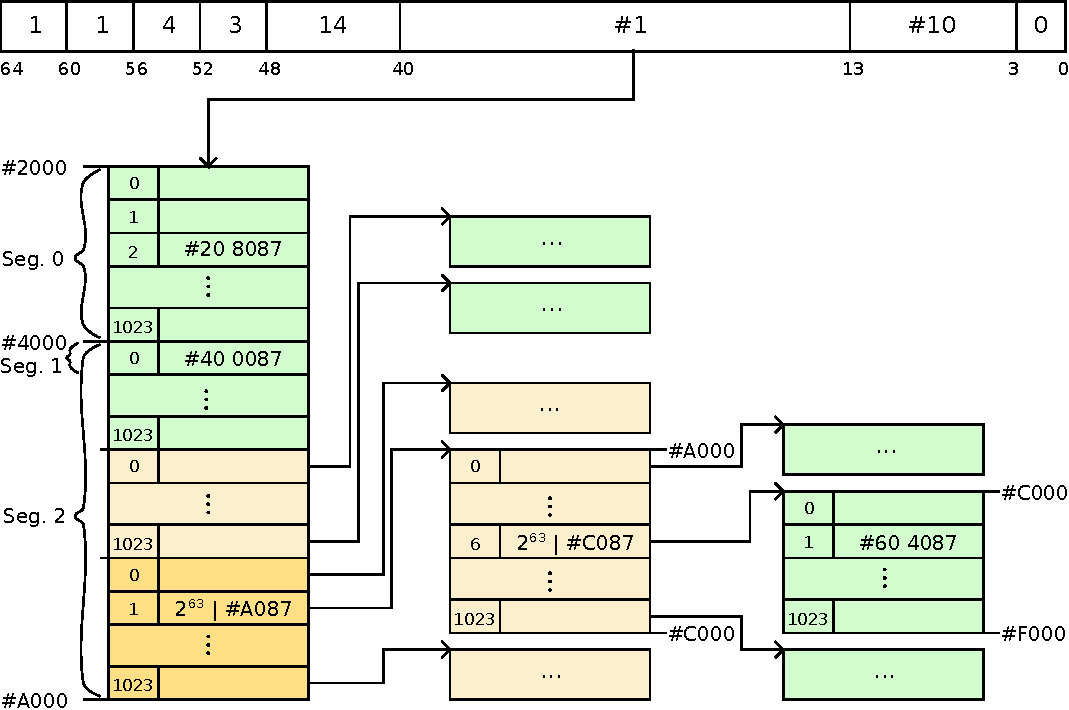
\includegraphics[width=\textwidth]{img/paging-example-crop.pdf}
	\caption{Paging example}
\end{figure}
\noindent Hence, segment 0 has 1024 pages, segment 1 has only one page, segment 2 has $1024^3$ pages and segment 3 has no pages at all. Additionally, the page size is $2^{14}$, the address space number is \haddr{10} and the root location is \haddr{2000} (\haddr{1}$~\ll 13$). The root location is displayed on the left, while auxiliary page tables are on the right. Furthermore, the green cells contain PTEs, the light orange cells PTPs of level 1 and the orange cells PTPs of level 2. For demonstration purposes, the cells display the page table index on the left and some show the content as an octa on the right. All PTEs and PTPs end with \haddr{87}, because they have to match the $n$ of \sr{V} and have read, write and execute permissions (which actually has no special reason here).

Ignoring the special case that segment 1 and 2 overlap for a while, one can see that the number of page tables in the root location for segment $i$ corresponds to $b_{i+1} - b_i$. The first page table does always contain PTEs, the second one PTPs of level 1 and so on. Each page table has 1024 slots and therefore it is 8192 bytes large. As the arrows show, PTPs do always point to another page table.

Since in this case $b_1$ is equal to $b_2$, segment 1 has only one page. An additional consequence of the interpretation of the segment sizes and the translation mechanism is, that -- as the figure shows -- the page in segment 1 is mapped by the first PTE of the page table responsible for segment 2. Thus, this PTE is used for the first page both in segment 1 and segment 2.

% TODO let's
To demonstrate the translation process, let's go through a few examples:
\begin{itemize}
	\item \haddr{80FF}:\\
	Obviously, \haddr{80FF} belongs to segment 0 and the page number is $(00002)_{1024}$. As described, in this case the PTE is \pmem{8}{2^{13}($\lstinline`\#1`$+0) + 8*2}$~=~$\pmemh{8}{2010}. The third slot of the first page table in segment 0 contains \haddrt{20}{8087}, which means that the physical base address for that page is \haddrt{20}{8000} and thus, the resulting physical address \haddrt{20}{80FF}.
	\item \haddro{2000}{0000}{0000}{1234}:\\
	This address belongs to segment 1 and has the page number $(00001)_{1024}$. The PTE is \pmem{8}{2^{13}($\lstinline`\#1`$+1) + 8*0}$~=~$\pmem{8}{$\lstinline`\#4000`$}$~=~$\haddrt{40}{0087}. Hence, the resulting physical address is \haddrt{40}{1234}.
	\item \haddro{4000}{0004}{0600}{4000}:\\
	Last but not least, this address belongs to segment 2 and has the page number $(00161)_{1024}$. Thus, the level 2 PTP is \pmem{8}{2^{13}($\lstinline`\#1`$+3) + 8*1}$~=~$\pmemh{8}{8008}, which loads \haddro{8000}{0000}{0000}{A087}. Therefore it links to the PTE \pmem{8}{$\lstinline`\#A000`$ + 8*6}$~=~$\pmemh{8}{A030}, which in turn is \haddro{8000}{0000}{0000}{C087}. The last step loads the PTE \pmem{8}{$\lstinline`\#C000`$ + 8*1} $=~$\pmemh{8}{C008}$~=~$\haddrt{60}{4087}, so that the final address is \haddrt{60}{4000}.
\end{itemize}

\subsubsection{Translation Caches}

To prevent that every memory access requires this lengthy translation from virtual to physical addresses, MMIX uses a \i{translation cache}. This is also known as \i{translation lookaside buffer} (TLB). However, MMIX calls it translation cache or short TC. The exact behaviour or whether separate caches for instructions and data exist, is not enforced by the architecture. But MMIX defines that the TC contains \i{translation keys}, which are associated with \i{translations}. The translation key is basically the virtual address, whereas the translation is more or less the physical address. The key is structured as follows:
\begin{figure}[H]
	\centering
	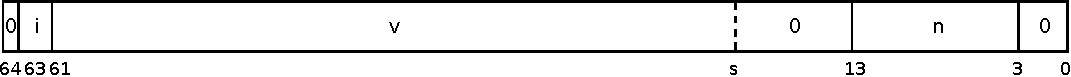
\includegraphics[width=\textwidth]{img/TC-key-crop.pdf}
\end{figure}
\vspace{-20pt}
\noindent As usual, the field $n$ holds the address space number. The field $i$ is the segment number and $v$ is the virtual address, divided by the page size. The other parts are defined to be zero. The layout of a translation is:
\begin{figure}[H]
	\centering
	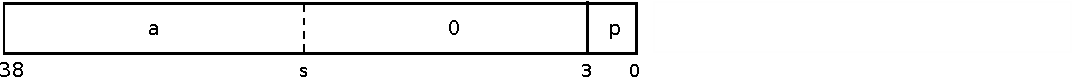
\includegraphics[width=\textwidth]{img/TC-trans-crop.pdf}
\end{figure}
\vspace{-20pt}
\noindent Similarly to a PTE, the field $a$ holds the physical address, divided by the page size. The last three bits contain the protection bits, whereas the other bits are defined to be zero. \citep[pg. 37]{mmix-doc}

Of course, the operating system needs a way to keep the TC up to date, when for example removing PTEs or changing their protection bits. Therefore, MMIX provides the instruction \mi{LDVTS}.

\instrtbl
	{\mi{LDVTS \$X,\$Y,\$Z|Z}}
	{$\dr{X} \leftarrow updateTC(\dr{Y} + \udrim{Z})$}
\noindent The instruction \i{load virtual translation status} updates the translation cache for $\dr{Y} + \udrim{Z}$, which should have the form of a translation key, except that the least significant three bits need not be zero. \dr{X} will be set to 0 if the key is not in the TC, 1 if it is present for instructions, 2 if it is present for data and 3 if it is present for both. If this key is present in the TC, the protection bits will be replaced with $(\dr{Y} + \udrim{Z})~\land~$\haddr{7}. If these are zero, the key will be removed. \citep[pg. 37]{mmix-doc}

\subsubsection{Physical Memory Caches}

As already mentioned, a particular implementation of MMIX may use caches for the RAM space of the physical memory. Which caches are present and how they are organized, is completely implementation dependent. But MMIX provides several instructions to allow a more efficient use of the caches and to keep them up to date. Similarly to the translation caches, MMIX has in mind that an implementation may provide separate caches for instructions and data.

\instrtbl
	{\mi{LDUNC \$X,\$Y,\$Z|Z}}
	{$\dr{X} \leftarrow s(\vmem{8}{\dr{Y} + \udrim{Z}})$}
\noindent The first instruction in this category is \mi{LDUNC}, \i{load octa uncached}. It has  the same behaviour as \mi{LDO}, but tells MMIX "that the loaded octabyte (and its neighbors in a cache block) will probably not be read or written in the near future" \citep[pg. 24]{mmix-doc}.

\instrtbl
	{\mi{STUNC \$X,\$Y,\$Z|Z}}
	{$\vmem{8}{\dr{Y} + \udrim{Z}}~\leftarrow s(\dr{X})$}
\noindent The instruction \i{store octa uncached} has the same meaning as \mi{STO} and tells MMIX the same as \mi{LDUNC} does. \citep[pg. 24]{mmix-doc}

\instrtbl
	{\mi{PRELD|PREGO|PREST X,\$Y,\$Z|Z}}
	{-}
\noindent These instructions have no (visible) effect, but inform MMIX that the ${\tt X}+1$ bytes \vmem{1}{\dr{Y} + \udrim{Z}}, \dots, \vmem{1}{\dr{Y} + \udrim{Z} + {\tt X}} will probably be loaded/stored, used as instructions or stored before loaded for \mi{PRELD}, \mi{PREGO} or \mi{PREST}, respectively. That means, if \mi{PRELD} is used, it might make sense to load these bytes into the data cache. If \mi{PREGO} is used, MMIX might put these bytes into the instruction cache and if \mi{PREST} is used, MMIX may ignore the current bytes in memory. Therefore, if these bytes are requested and are not yet in cache, MMIX does not need to load them from memory, because they will be written before they are read anyway. MMIX does also define, that no protection fault occurs for these instructions. \citep[pg. 24]{mmix-doc}

\instrtbltwo
	{\mi{SYNCD X,\$Y,\$Z|Z}}
	{$caches[\dr{Y} + \udrim{Z}:{\tt X}+1] \rightarrow$~\pmem{}{\dr{Y} + \udrim{Z}:{\tt X}+1}}
	{if in privileged mode: $caches[\dr{Y} + \udrim{Z}:{\tt X}+1] \leftarrow \varnothing$}
\noindent The instruction \i{synchronize data} forces the hardware to make sure that all data for the ${\tt X}+1$ bytes \vmem{1}{\dr{Y} + \udrim{Z}}, \dots, \vmem{1}{\dr{Y} + \udrim{Z} + {\tt X}} is present in memory (and not only in cache). If executed in the privileged space, it does additionally force MMIX to remove these bytes from the data cache. Again, no protection fault will occur if the memory is not accessible. \citep[pg. 24]{mmix-doc}

\instrtblfour
	{\mi{SYNCID X,\$Y,\$Z|Z}}
	{if in user mode:}
	{$\quad IC[\dr{Y} + \udrim{Z}:{\tt X}+1] \leftrightarrow DC[\dr{Y} + \udrim{Z}:{\tt X}+1]$}
	{else:}
	{$\quad caches[\dr{Y} + \udrim{Z}:{\tt X}+1] \leftarrow \varnothing$}
\noindent When executed in user space, \i{synchronize instructions and data} forces the hardware to make sure that the ${\tt X}+1$ bytes \vmem{1}{\dr{Y} + \udrim{Z}}, \dots, \vmem{1}{\dr{Y} + \udrim{Z} + {\tt X}} will be interpreted correctly when used as instructions. That means, MMIX should synchronize its data cache with its instruction cache (\eg because instructions might have been manually fabricated and might thus only be present in the data cache yet). When \mi{SYNCID} is executed in privileged space, the hardware has to remove these bytes from all caches \i{without} writing it to memory. As with \mi{SYNCD}, no protection faults can occur. \citep[pg. 24,25]{mmix-doc}

\instrtbleight
	{\mi{SYNC XYZ}}
	{if ${\tt XYZ} = 0$: drain pipeline}
	{if ${\tt XYZ} = 1$: drain stores}
	{if ${\tt XYZ} = 2$: drain loads}
	{if ${\tt XYZ} = 3$: drain loads and stores}
	{if ${\tt XYZ} = 4$: go into power-saver mode}
	{if ${\tt XYZ} = 5$: flush caches to memory}
	{if ${\tt XYZ} = 6$: clear TCs}
	{if ${\tt XYZ} = 7$: clear caches}
\noindent The last instruction in this category is \i{synchronize}, which is used for various purposes, whereas the 24-bit constant {\tt XYZ} determines what action is performed. The first four actions drain the pipeline, in the sense that it stalls until all preceding instructions are finished (or all stores, loads, loads and stores for 1, 2, 3, respectively, are finished before the corresponding instructions after them). The fifth action tells MMIX to go into a power-saver mode, \ie MMIX is allowed to execute instructions slower or not at all until some kind of signal arrives. The next one writes all cache content to main memory, while the last two simply remove all entries from the TCs or the instruction and data caches. Using \mi{SYNC} with ${\tt XYZ} > 3$ is allowed in privileged mode only. \citep[pg. 25]{mmix-doc}


\section{Floating Point Operations}

Besides integer arithmetic, MMIX does also provide instructions to work with floating point numbers. The floating point arithmetic respects the IEEE/ANSI Standard 754. Since 64-bit quantities are the words of MMIX, arithmetic does always work with 64-bit floats, \ie "doubles". But MMIX does also support some instructions to convert from 64-bit floats to 32-bit floats and the other way around.

\subsection{Representation of Floating Point Numbers}

A 64-bit floating point number has the following structure:
\begin{figure}[H]
	\centering
	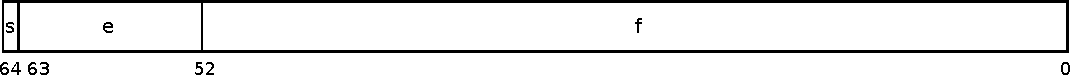
\includegraphics[width=\textwidth]{img/float-crop.pdf}
\end{figure}
\vspace{-20pt}
\noindent That means, it has a sign-bit $s$, an 11-bit exponent $e$ and a 52-bit fraction $f$. Taking $e$ as an unsigned integer and $f$ as a fraction between 0 and $(.111\dots1)_2 = 1 - 2^{-52}$, an octabyte has the following significance:
$$\vbox{\halign{\hfil$\pm#$,\quad if &#\hfil\cr
	0.0								& $e = f = 0$ (zero);\cr
	2^{\mkern1mu e - 1023}(1 + f)	& $0 < e < 2047$ (normal);\cr
	2^{-1022}f						& $e = 0$ and $f > 0$ (subnormal);\cr
	\infty							& $e = 2047$ and $f = 0$ (infinite);\cr
	\NaN(f)							& $e = 2047$ and $0 < f < 1/2$ (signaling NaN);\cr
	\NaN(f)							& $e = 2047$ and $f \ge 1/2$ (quiet NaN).\cr
}}$$
As shown, there are two representations for zero - a positive and a negative one. There are \i{normal} numbers, that can range from approximately $\pm 10^{-308}$ to $\pm 10^{308}$. Additionally \i{subnormal} numbers (also called \i{denormal} or \i{denormalized} numbers) are supported, which can range from approximately $\pm 10^{-324}$ to $\pm 10^{-308}$, but have fewer bits of precision. If the exponent has the maximum value, \ie 2047, it encodes infinity or \i{not a number} (\NaN). The latter distinguishes between \i{signaling} and \i{quiet} \NaN. Signaling \NaNs raise an invalid \glslink{Exception}{AE} when they are used, while quiet \NaNs won't. \citep[pg. 15]{mmix-doc}

Furthermore, the standard defines that four rounding modes should be available: round to nearest (and to even in case of ties, \ie the least significant bit should be zero), round off (toward zero), round up (toward $+\infty$) and round down (toward $-\infty$). MMIX uses the special register \sr{A} to specify the rounding mode. Additionally, all instructions having only one operand, specify the rounding mode with operand {\tt Y} using ${\tt Y}=0$ for the round mode in \sr{A}, ${\tt Y}=1$ for round off, ${\tt Y}=2$ for round up, ${\tt Y}=3$ for round down and ${\tt Y}=4$ for round near. \citep[pg. 15 and 21]{mmix-doc}

Last but not least, there are five kinds of \glslink{Exception}{arithmetic exceptions}, that can occur when working with floating point numbers:
\begin{enumerate}
	\item Floating overflow (value too large to be representable),
	\item Floating underflow (value too small to be representable),
	\item Floating divide by zero,
	\item Floating inexact (exact result not representable) and
	\item Floating invalid (square root of negative number, using signaling \NaN, \dots).
\end{enumerate}
As already said, all of these will either raise an \glslink{Exception}{AE} or set the corresponding \i{event bit} in \sr{A}, depending on whether the corresponding \i{enable bit} in \sr{A} is set or not. \citep[pg. 15]{mmix-doc}

\subsection{Arithmetic}

The first category of floating point operations are the arithmetic instructions. The floating point instructions don't have an \glslink{Immediate Value}{immediate} version, because it doesn't make much sense to specify a float with a single byte. Additionally, this section uses $f(\dots)$ to indicate that a value is interpreted as a 64-bit floating point number.

\instrtbl
	{\mi{FADD|FSUB \$X,\$Y,\$Z}}
	{$\dr{X} \leftarrow f(\dr{Y}) +|- f(\dr{Z})$}
\noindent \mi{FADD} computes the sum of \dr{Y} and \dr{Z}, treating them as floating point numbers and puts the result in \dr{X}. \mi{FSUB} performs the same operation, but switches the sign of \dr{Z} first, if \dr{Z} is not \NaN. If the sum of $(+\infty)+(-\infty)$ or $(-\infty)+(+\infty)$ is computed, an invalid \glslink{Exception}{AE} will be raised. \citep[pg. 16]{mmix-doc}

\instrtbl
	{\mi{FMUL|FDIV \$X,\$Y,\$Z}}
	{$\dr{X} \leftarrow f(\dr{Y}) *|/ f(\dr{Z})$}
\noindent These instructions multiply or divide the floating point numbers \dr{Y} and \dr{Z}. Several cases result in an invalid \glslink{Exception}{AE}, like $(\pm 0.0)*(\pm \infty)$, $(\pm 0.0)/(\pm 0.0)$ or $(\pm \infty)/(\pm \infty)$. Of course, dividing by $(\pm 0.0)$ raises a floating divide by zero \glslink{Exception}{AE}. \citep[pg. 16]{mmix-doc}

\instrtbl
	{\mi{FREM \$X,\$Y,\$Z}}
	{$\dr{X} \leftarrow f(\dr{Y}) \bmod f(\dr{Z})$}
\noindent The \i{floating remainder} instruction computes the remainder and puts it into \dr{X}. This is defined "to be $\dr{Y} - n * \dr{Z}$, where $n$ is the nearest integer to $\dr{Y}/\dr{Z}$, and $n$ is an even integer in case of ties" \citep[pg. 16]{mmix-doc}. If \dr{Y} is infinite and/or \dr{Z} is zero, an invalid \glslink{Exception}{AE} will be raised. \citep[pg. 16]{mmix-doc}

\instrtbl
	{\mi{FSQRT \$X,Y,\$Z}}
	{$\dr{X} \leftarrow \sqrt{f(\dr{Z})},\quad$ using round-mode {\tt Y}}
\noindent The last one in this family is \i{floating square root}. It puts the square root of \dr{Z} into \dr{X}. An invalid \glslink{Exception}{AE} is raised will be \dr{Z} is negative, except for $-0.0$. \citep[pg. 17]{mmix-doc}

\subsection{Comparison}

Of course, besides doing arithmetic, one has to be able to compare floating point numbers. This does not work well using the integer comparison instructions, because one would have to take care of negative numbers, $+0.0$, $-0.0$ and \NaN manually. Therefore, the floating point comparisons simplify that task.

\instrtbl
	{\mi{FCMP \$X,\$Y,\$Z}}
	{$\dr{X} \leftarrow (f(\dr{Y}) > f(\dr{Z})) - (f(\dr{Y}) < f(\dr{Z}))$}
\noindent As the effect description shows, \mi{FCMP} is basically the same as \mi{CMP}, but treats the operands as floating point numbers. Thus, \dr{X} will be set to $-1$, if \dr{Y} is less than \dr{Z}, 0 if \dr{Y} is equal to \dr{Z} and 1 if \dr{Y} is greater than \dr{Z}. It will raise an invalid \glslink{Exception}{AE} and set \dr{X} to zero, if \dr{Y} or \dr{Z} is \NaN. \citep[pg. 17]{mmix-doc}

\instrtbl
	{\mi{FEQL \$X,\$Y,\$Z}}
	{$\dr{X} \leftarrow (f(\dr{Y}) = f(\dr{Z}))~?~1~:~0$}
\noindent \i{Floating equal to} sets \dr{X} to 1, if \dr{Y} and \dr{Z} are equal. But it is noteworthy, that \NaN is not equal to anything and $-0.0$ is equal to $+0.0$. \citep[pg. 17]{mmix-doc}

\instrtbl
	{\mi{FUN \$X,\$Y,\$Z}}
	{$\dr{X} \leftarrow (f(\dr{Y}) = \NaN \lor f(\dr{Z}) = \NaN)~?~1~:~0$}
\noindent The last comparison instruction is \i{floating unordered} and sets \dr{X} to 1, if \dr{Y} and \dr{Z} are considered \i{unordered}, \ie at least one of them is \NaN. \citep[pg. 17]{mmix-doc}

\subsection{Neighborhood Comparison}

Because of the limited precision of floating point numbers, operations might produce inexact results. The larger the numbers, the larger the potential difference of the produced result to the exact result. For that reason, an absolute comparison of floats, as the last section described, is not always desired. Therefore, MMIX offers another category of instructions that allow comparisons with respect to an \i{epsilon} and depending on the magnitude of the floating point numbers in question.

At first, MMIX defines a so called \i{neighborhood} of a number. Assuming that epsilon is a float called $\epsilon$, the float $u$ with fraction $f$ and exponent $e$ has the neighborhood:
\[
	N_\epsilon(u) = \left\{
	\begin{array}{l l}
		\{x \mid |x-u| \le 2^{e-1022}\epsilon\}
			& \quad \text{if $u$ is normal}\\
		\{x \mid |x-u| \le 2^{-1021}\epsilon\}
			& \quad \text{if $u$ is subnormal}\\
		\{0\}
			& \quad \text{if $u$ is zero}\\
		\{\pm \infty\}
			& \quad \text{if $u$ is $\pm \infty$ and $\epsilon < 1$}\\
		\{\text{everything except $\mp \infty$}\}
			& \quad \text{if $u$ is $\pm \infty$ and $1 \le \epsilon < 2$ and}\\
		\{\text{everything}\}
			& \quad \text{if $u$ is $\pm \infty$ and $\epsilon \ge 2$.}\\
	\end{array} \right.
\]
\citep[pg. 19]{mmix-doc} Without going into the details of this definition, it basically means that the neighborhood of a normal float depends on its exponent. That is, the larger the exponent, the larger the neighborhood.

Displayed graphically (and a bit exaggerated for demonstration purposes), the neighborhoods of a few numbers might look like the following:
\begin{figure}[H]
	\centering
	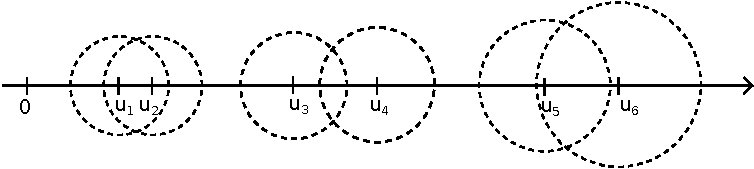
\includegraphics[width=\textwidth]{img/cmpe-less-crop.pdf}
	\caption{Example neighborhoods, demonstrating float relationships}
\end{figure}
\noindent MMIX distinguishes four cases when comparing floats $u$ and $v$ with respect to $\epsilon$:
\begin{enumerate}
	\item $u \approx v$, if $u \in N_\epsilon(v)$ and $v \in N_\epsilon(u)$.\\
	That means, two numbers will be considered \i{equivalent}, if both are in the neighborhood of the corresponding other number. In the example, only $u_1 \approx u_2$, because $u_1 \in N_\epsilon(u_2)$ and $u_2 \in N_\epsilon(u_1)$.
	\item $u \sim v$, if $u \in N_\epsilon(v)$ or $v \in N_\epsilon(u)$.\\
	Thus, two numbers will be considered \i{similar}, if only one of them belongs to the neighborhood of the corresponding other number. For example, $u_5 \sim u_6$, because $u_5 \in N_\epsilon(u_6)$, but $u_6 \notin N_\epsilon(u_5)$.
	\item $u \prec v$, if $u < N_\epsilon(v)$ and $N_\epsilon(u) < v$.\\
	For example, $u_3 \prec u_4$ because $u_3$ is less than all numbers in $N_\epsilon(u_4)$ and all numbers in $N_\epsilon(u_3)$ are less than $u_4$.
	\item $u \succ v$, if $u > N_\epsilon(v)$ and $N_\epsilon(u) > v$.\\
	Analogous, $u_4 \succ u_3$.
\end{enumerate}
\citep[pg. 19]{mmix-doc} The following instructions are based on this definition and use the special \i{epsilon register} \sr{E} for $\epsilon$.

\instrtbl
	{\mi{FCMPE \$X,\$Y,\$Z}}
	{$\dr{X} \leftarrow (f(\dr{Y}) \succ f(\dr{Z})~(\sr{E})) - (f(\dr{Y}) \prec f(\dr{Z})~(\sr{E}))$}
\noindent Analogous to \mi{FCMP}, \mi{FCMPE} - called \i{floating compare with respect to epsilon} - compares \dr{Y} with \dr{Z} according to the definition above and sets \dr{X} to $-1$, 0 or 1. It should be noted, that \dr{X} will be set to zero, if \dr{Y} is similar \i{or} equivalent to \dr{Z}. An invalid \glslink{Exception}{AE} will be raised, if \dr{Y}, \dr{Z} or \sr{E} is \NaN or \sr{E} is negative. \citep[pg. 19]{mmix-doc}

\instrtbl
	{\mi{FEQLE \$X,\$Y,\$Z}}
	{$\dr{X} \leftarrow (f(\dr{Y}) \approx f(\dr{Z})~(\sr{E}))~?~1~:~0$}
\noindent Similarly to \mi{FEQL}, \mi{FEQLE} will set \dr{X} to 1, if \dr{Y} is equivalent to \dr{Z}, depending on \sr{E}. It raises the same \glslink{Exception}{arithmetic exceptions} as \mi{FCMPE}. \citep[pg. 19]{mmix-doc}

\instrtbl
	{\mi{FUNE \$X,\$Y,\$Z}}
	{$\dr{X} \leftarrow (f(\dr{Y}) = \NaN \lor f(\dr{Z}) = \NaN \lor \sr{E} = \NaN \lor \sr{E} < 0)~?~1~:~0$}
\noindent The last one in this group is \mi{FUNE}, which will set \dr{X} to 1, if \dr{Y}, \dr{Z} or \sr{E} are exceptional as described for \mi{FCMPE} and \mi{FEQLE}. \citep[pg. 19]{mmix-doc}

\subsection{Conversion between Float and Integer}

MMIX offers three groups of instructions to convert an integer to a floating point number and the other way around.

\instrtbl
	{\mi{FIX|FIXU \$X,Y,\$Z}}
	{$\dr{X} \leftarrow (int)f(\dr{Z}) \bmod 2^{64},\quad$ using round-mode {\tt Y}}
\noindent The instructions \i{convert floating to fixed} and \i{convert floating to fixed unsigned} take \dr{Z} as a float, convert it to an integer and put it into \dr{X}. Only when using \mi{FIX}, an invalid \glslink{Exception}{AE} will be raised if \dr{Z} is infinite or \NaN and a float-to-fix \glslink{Exception}{AE} will occur, if the result is less than $-2^{63}$ or greater than $2^{63}-1$. \citep[pg. 20]{mmix-doc}

\instrtbl
	{\mi{FINT \$X,Y,\$Z}}
	{$\dr{X} \leftarrow f((int)f(\dr{Z})),\quad$ using round-mode {\tt Y}}
\noindent The instruction \i{floating integer} rounds the float \dr{Z} to a floating integer and places it in \dr{X}. Infinity and \NaN are not changed. The difference to \mi{FIX} is, that \mi{FINT} writes a floating point number to \dr{X}, while \mi{FIX} writes a signed integer to \dr{X}. \citep[pg. 17]{mmix-doc}

\instrtbl
	{\mi{FLOT|FLOTU \$X,Y,\$Z|Z}}
	{$\dr{X} \leftarrow f(\sdrimm{Z}),\quad$ using round-mode {\tt Y}}
\noindent Finally, the instructions \i{convert fixed to floating} and \i{convert fixed to floating unsigned} treat \udrim{Z} as an integer and convert it to the nearest floating point number. Only if using \mi{FLOT}, an floating inexact \glslink{Exception}{AE} will be raised, if rounding is necessary. \citep[pg. 20]{mmix-doc}

\subsection{Short Floats}

Although MMIX is a 64-bit architecture and thus, works with 64-bit floating point values by default, it does also provide some instructions to use 32-bit floating point numbers, called \i{short floats}. But MMIX has no separate arithmetic, comparison and other instructions for them. Instead it offers instructions to load a short float from memory into a float and store a float as a short float to memory.

\instrtbl
	{\mi{LDSF \$X,\$Y,\$Z|Z}}
	{$\dr{X} \leftarrow f(sf(\vmem{4}{\dr{Y} + \udrim{Z}}))$}
\noindent The first one, called \i{load short float}, loads the tetra \vmem{4}{\dr{Y} + \udrim{Z}}, treating it as a 32-bit float, converts it to a 64-bit float and puts it into \dr{X}. \citep[pg. 20]{mmix-doc}

\instrtbl
	{\mi{STSF \$X,\$Y,\$Z|Z}}
	{$\vmem{4}{\dr{Y} + \udrim{Z}}~\leftarrow sf(f(\dr{X}))$}
\noindent \mi{STSF} goes the other way: it treats \dr{X} as a 64-bit float, converts it to a 32-bit float and stores that into \vmem{4}{\dr{Y} + \udrim{Z}}. It may trigger a floating overflow, underflow, inexact and invalid \glslink{Exception}{AE}. \citep[pg. 20]{mmix-doc}

\instrtbl
	{\mi{SFLOT|SFLOTU \$X,Y,\$Z|Z}}
	{$\dr{X} \leftarrow f(sf(\sdrimm{Z})),\quad$ using round-mode {\tt Y}}
\noindent These instructions behave like \mi{FLOT} and \mi{FLOTU}, but convert \sdrim{Z} to a 32-bit float first, which ensures that no \glslink{Exception}{AE} will be raised if \dr{X} is stored with \mi{STSF} afterwards. \citep[pg. 20]{mmix-doc}



\section{Register Stack}

Actually, the local registers in MMIX are more complicated than explained at the beginning. Because MMIX uses a combination of registers and memory for the stack. This way, \glslink{Subroutine linkage}{subroutine linkage} is realized. Additionally, MMIX offers instructions to save or restore the complete state of a running program using the stack. Both are explained in detail in this section.

\subsection{Subroutine Linkage}

Because of the complexity of the \glslink{Subroutine linkage}{subroutine linkage} mechanism, it is explained in two steps. At first, it is shown from the perspective of the programmer. Afterwards the internal functional principle is described.

\subsubsection{Programmers View}

The programmer has \sr{G} local registers named \dr{0}, \dots, \dr{(\sr{G} - 1)} at his hand. The registers \dr{0}, \dots, \dr{(\sr{L} - 1)} are the currently used ones, while \dr{(\sr{L})}, \dots, \dr{(\sr{G} - 1)} are the marginal registers. Furthermore he can think of the stack as an potentially unbounded list $S$. The stack pointer, \ie the pointer that indicates the slot in $S$ that is going to be written next, is called $\tau$, which is initially zero. \citep[pg. 22]{mmix-doc}

\paragraph{Calling and Returning}

MMIX provides two instruction families to call subroutines and return from them.

\instrtblseven
	{\mi{PUSHJ \$X,@+4*(YZ[-$2^{16}$]),\quad PUSHGO \$X,\$Y,\$Z|Z}}
	{$S[\tau] \leftarrow \dr{0}, S[\tau+1] \leftarrow \dr{1}, \dots, S[\tau + {\tt X} - 1] \leftarrow \dr{(X - 1)}$}
	{$S[\tau + {\tt X}] \leftarrow {\tt X}$}
	{$\tau \leftarrow \tau + {\tt X} + 1$}
	{$\dr{0} \leftarrow \dr{X + 1}, \dr{1} \leftarrow \dr{X + 2},\dots, \dr{(\sr{L} - X - 2)} \leftarrow \dr{(\sr{L} - 1)}$}
	{$\sr{L} \leftarrow \sr{L} - {\tt X} - 1$}
	{$\sr{J} \leftarrow @ + 4$}
	{$@ \leftarrow (@+4*({\tt YZ}[-2^{16}]))~|~(\dr{Y} + \udrim{Z})$}
\noindent At first, \mi{PUSHJ} (\i{push registers and jump}) and \mi{PUSHGO} (\i{push registers and go}) are essentially the same, except that MMIX determines the new value of the \glslink{PC}{instruction pointer} in different ways. The first action they perform is to push the current local registers \dr{0}, \dots, \dr{(X - 1)} onto the stack $S$. Afterwards the number of registers, that have been \i{pushed down}, is saved in $S[\tau + {\tt X}]$ and $\tau$ is increased correspondingly. The next step is to rename the current registers \dr{(X + 1)}, \dots, \dr{(\sr{L} - 1)} to \dr{0}, \dots, \dr{(\sr{L} - X - 2)}. That means, all used registers above {\tt X} are passed as arguments to the subroutine, where they appear as \dr{0}, \dr{1} and so on. Finally, \sr{L} is adjusted, so that only the arguments are currently in use, the \i{return-jump register} \sr{J} is set to the instruction that would have been executed normally and the \glslink{PC}{instruction pointer} is changed. \citep[pg. 22]{mmix-doc}

\instrtblseven
	{\mi{POP X,YZ}}
	{$x \leftarrow S[\tau - 1] \bmod 256$}
	{$S[\tau - 1] \leftarrow \dr{(X - 1)}$}
	{$\sr{L} \leftarrow min(x + {\tt X},\sr{G})$}
	{$\dr{(\sr{L} - 1)} \leftarrow \dr{(\sr{L} - x - 2)}, \dots \dr{(x + 1)} \leftarrow \dr{0}$}
	{$\dr{x} \leftarrow S[\tau - 1], \dr{(x - 1)} \leftarrow S[\tau - 2], \dots, \dr{0} \leftarrow S[\tau - x - 1]$}
	{$\tau \leftarrow \tau - x - 1$}
	{$@ \leftarrow \sr{J} + 4*{\tt YZ}$}
\noindent Of course, \mi{POP} (\i{pop registers and return from subroutine}) basically behaves in the opposite way as \mi{PUSHJ} and \mi{PUSHGO} do. At first, the number of registers that have been pushed down by the associated \mi{PUSHJ} or \mi{PUSHGO} are loaded from $S[\tau - 1]$. It can not be more than 255, because MMIX has only 256 dynamic registers. In the next step, MMIX sets $S[\tau - 1]$ to the "main return value" \dr{(X - 1)}, which is used later. Next, \sr{L} is adjusted to be the number of local registers the caller wanted to keep plus the number of return values, denoted by {\tt X}. Of course, that should not be more than \sr{G}. Subsequently, the registers holding the return values (except the main return value) are renamed, so that they appear in \dr{(x + 1)}, \dots, \dr{(\sr{L} - 1)} for the caller. Finally, the previously saved values are restored from the stack, $\tau$ is adjusted correspondingly and MMIX jumps back to the location stored in \sr{J}. Optionally, some instructions can be skipped with ${\tt YZ} > 0$. It is noteworthy that the main return value appears in the so called \i{hole} \dr{x}, \ie the register that has stored the number of registers that have been pushed down. \citep[pg. 22,23]{mmix-doc}

\paragraph{Example}

To make the just described instructions more clear, the following goes through an example. It supposes, that the first four local registers have some values and a \mi{PUSHJ \$1,Sub} is executed. The following figure illustrates the state before the \mi{PUSHJ} and the state afterwards, \ie the initial state in subroutine \i{Sub}:
\begin{figure}[H]
	\centering
	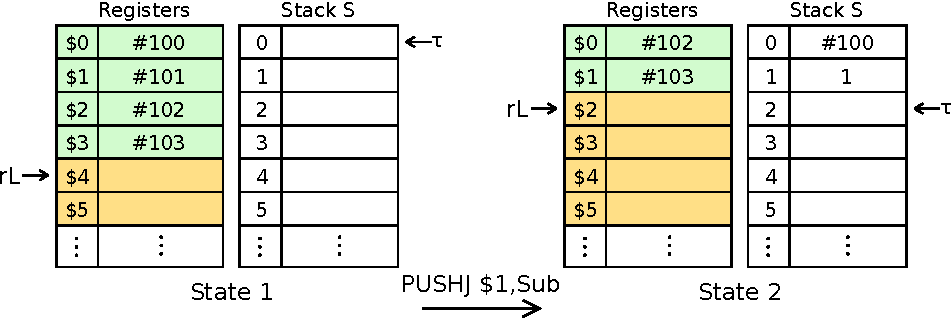
\includegraphics[width=\textwidth]{img/push-pop-user1-crop.pdf}
	\caption{Register stack: User perspective, state 1 to 2}
	\label{figure:push-pop-user1}
\end{figure}
\noindent The figure displays the used local registers green and the marginal ones orange. At first \dr{0} and \dr{1} are saved on the stack, whereas \dr{1} has been set to the number of pushed down values. Afterwards \dr{2} and \dr{3} are pushed as arguments to \i{Sub}, appearing as \dr{0} and \dr{1}. Thus, \sr{L} is 2 and $\tau$ is 2 as well.

In the next step of the example \i{Sub} performs some calculations, leading to state 3, and executes a \mi{POP 4,0} to return to the caller, whose state is shown on the right:
\begin{figure}[H]
	\centering
	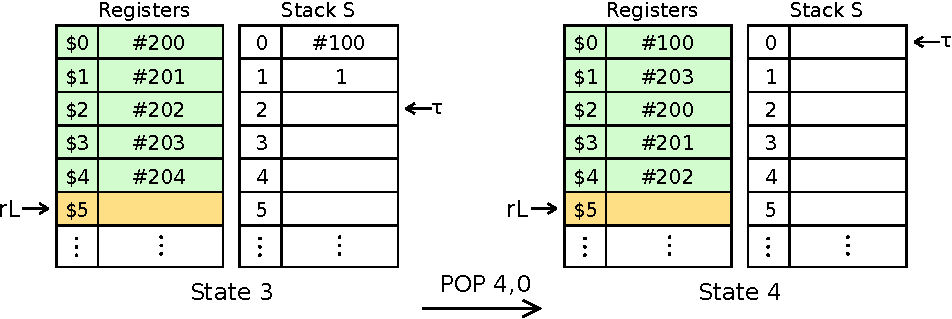
\includegraphics[width=\textwidth]{img/push-pop-user2-crop.pdf}
	\caption{Register stack: User perspective, state 3 to 4}
	\label{figure:push-pop-user2}
\end{figure}
\noindent As the figure shows, \dr{0}, \dots, \dr{4} have been set to some arbitrary values. The subsequent \mi{POP 4,0} at first loads the number of pushed down registers from the stack, \ie $S[\tau - 1] = 1$. Based on that, it restores \haddr{100} from $S[0]$ into \dr{0}, sets the hole (\dr{1}) to the last return value \haddr{203} and \dr{2}, \dots, \dr{4} to the other return values in the original order. Thus, \sr{L} is $1+{\tt X} = 5$ and $\tau$ is zero again.

At this point it might look strange that the last return value appears first for the caller, followed by the other ones in the same order they were in the registers of \i{Sub}. The section about the internal view will show the reason for that behaviour.

\paragraph{Special Cases}

Unfortunatly it is even more complicated as just described, because some special cases have been suppressed. The instructions \mi{PUSHJ|PUSHGO \$X,\dots} have the following special cases:
\begin{itemize}
	\item If $\sr{L} \le {\tt X} < \sr{G}$, the value of \sr{L} will be increased to ${\tt X} + 1$ first.
	\item If ${\tt X} \ge \sr{G}$, all local registers \dr{0}, \dots, \dr{(\sr{L} - 1)} will be saved, followed by \sr{L} and \sr{L} will be reset to zero.
\end{itemize}
On the other hand, \mi{POP X,YZ} has to take care of:
\begin{itemize}
	\item If ${\tt X} > \sr{L}$, {\tt X} will be replaced by $\sr{L} + 1$ first and the hole will be set to zero.
	\item If ${\tt X} = 0$, the hole will disappear, \ie it will become marginal.
\end{itemize}
\citep[pg. 22,23]{mmix-doc}

\subsubsection{Internal View}

After having described the procedure of calling subroutines and returning from them from the perspective of the programmer, it should be explained how MMIX does actually achieve that.

As mentioned previously, MMIX has a local register array $l$ with either 256, 512 or 1024 slots. It is used as a ring, which means that if we have the local registers $l[0]$, $l[1]$, \dots, $l[255]$, register $l[256]$ will be the same as $l[0]$, $l[257]$ the same as $l[1]$ and so on.

To realize the register stack, MMIX has to manage the registers and the stack in memory. To do so, the register ring is divided into three parts by $\alpha$, $\beta$ and $\gamma$. $l[\alpha]$, $l[\alpha+1]$, \dots, $l[\beta-1]$ are corresponding to \dr{0}, \dr{1}, \dots, \dr{(rL - 1)}. The registers $l[\beta]$, \dots, $l[\gamma-1]$ are currently unused and $l[\gamma]$, \dots, $l[\alpha-1]$ are the registers that are currently not accessible, called \i{hidden}, but have not yet been stored to memory. The situation on the stack in memory is described by the special registers \sr{O} and \sr{S}. The former is the offset of \dr{0} in memory, \ie the location it would be written to. The latter is the location the next register is going to be written to. $\alpha$, $\beta$ and $\gamma$ relate to \sr{O} and \sr{S} in the following way (when $2^n$ is the number of slots in $l$):
$$\rm\alpha=(rO/8)\bmod2^n,\qquad \beta=(\alpha+rL)\bmod2^n,\qquad
\hbox{and}\qquad \gamma=(rS/8)\bmod2^n$$

To make sure that no value is lost, MMIX has to take care that $\alpha$, $\beta$ and $\gamma$ never move past each other. Whenever a \mi{PUSHJ|PUSHGO} is done, $\alpha$ moves towards $\beta$. Setting \dr{X} with ${\tt X} \ge \sr{L}$ means that \sr{L} is increased, \ie $\beta$ is moved towards $\gamma$. If $\beta$ moved past $\gamma$, registers would have to be written to memory first to free as many slots as required. To do so, $l[\gamma]$ is written to \vmem{8}{\sr{S}} and $\gamma$ is increased by one and thus \sr{S} by 8, until the new $\beta$ is less than $\gamma$. When doing a \mi{POP}, $\alpha$ moves backwards to $\gamma$. If this moved $\alpha$ past $\gamma$, we would have to load values back from memory first. That means, $\gamma$ and \sr{S} are decreased and \vmem{8}{\sr{S}} is put into $l[\gamma]$ until the new $\alpha$ is less than $\gamma$. \citep[pg. 33]{mmix-doc}

The following figures illustrate the actions with a similar example as in the previous section. For simplicity it is assumed that only 4 local registers are present\footnote{This is not specification conform, as explained previously, but simplifies the example.}:
\begin{figure}[H]
	\centering
	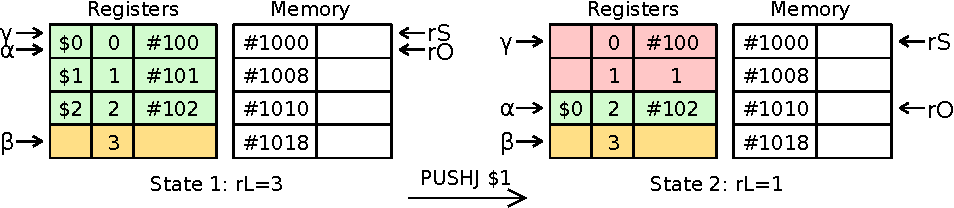
\includegraphics[width=\textwidth]{img/push-pop-internal1-crop.pdf}
	\caption{Register stack: Internal perspective, state 1 to 2}
	\label{figure:push-pop-internal1}
\end{figure}
\noindent The green and yellow cells have the same meaning as in figures \ref{figure:push-pop-user1} and \ref{figure:push-pop-user2}, while the red cells are the hidden registers. The register block on the left shows the current assignment of dynamic registers, the local register index and the value in the register. The right block displays the stack in memory with the address and the value. Additionally the values of $\alpha$, $\beta$, $\gamma$, \sr{O} and \sr{S} are indicated by pointing to the corresponding register or memory slot.

In the first state, three registers are used, $\alpha$ and $\gamma$ are zero, $\beta$ is $\alpha+\sr{L} = 3$ and \sr{O} and \sr{S} have the value \haddr{1000}. State 2 is reached by doing a \mi{PUSHJ \$1}. Hence, the offset $\alpha$ in the register ring is increased by 2 and the offset \sr{O} in memory is increased by 16. Additionally, the hole ($l[1]$) is set to the number of registers that have been pushed down.

\begin{figure}[H]
	\centering
	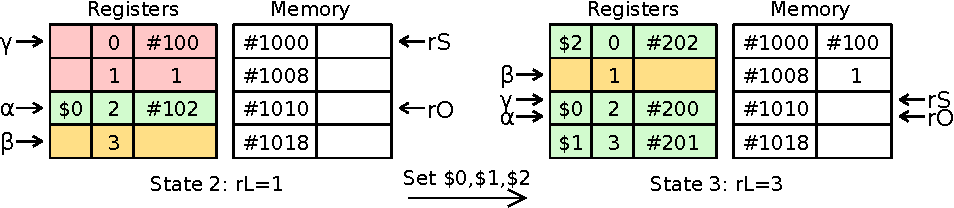
\includegraphics[width=\textwidth]{img/push-pop-internal2-crop.pdf}
	\caption{Register stack: Internal perspective, state 2 to 3}
	\label{figure:push-pop-internal2}
\end{figure}
\noindent The third state, shown in figure \ref{figure:push-pop-internal2}, is reached by setting \dr{0}, \dr{1} and \dr{2} to \haddr{200}, \haddr{201} and \haddr{202}, respectively. Setting \dr{0} does not increase \sr{L}, so that only $l[2]$ is changed. The other two both increase \sr{L} by one, \ie move $\beta$ towards $\gamma$. Thus, in each case $\gamma$ and \sr{S} are increased and a value is written to memory.

\begin{figure}[H]
	\centering
	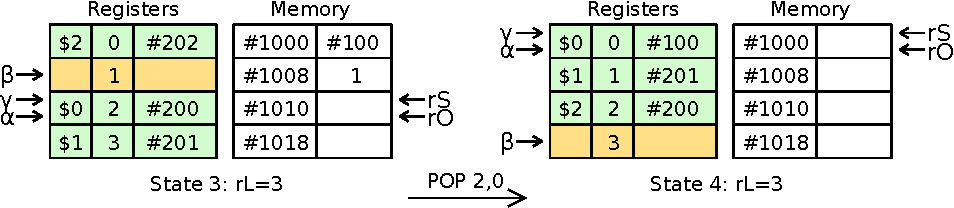
\includegraphics[width=\textwidth]{img/push-pop-internal3-crop.pdf}
	\caption{Register stack: Internal perspective, state 3 to 4}
	\label{figure:push-pop-internal3}
\end{figure}
\noindent The last transition, illustrated in figure \ref{figure:push-pop-internal3}, is achieved by doing a \mi{POP 2,0}. As described, \mi{POP} moves $\alpha$ back. The hole tells MMIX how many registers have been pushed down by the preceding \mi{PUSHJ} or \mi{PUSHGO}. In this case, the hole has been written to memory, so that it has to be loaded back first. Afterwards MMIX has to move $\alpha$ two steps up because one register has been saved and the hole has been created. To be able to decrease $\alpha$ and \sr{O}, one further value has to be loaded from memory. To return the two values, a move of $l[3]$ to $l[1]$ is sufficient because the other value is already in the desired slot (as all other return values would be, if there were more than two). This is the reason for the -- at a first glance -- strange order of the return values.

\subsection{Saving and Restoring the State}

Another concept, that works with the register stack as well, is the procedure of storing and restoring the state of the running program. It is intended both for the operating system and user applications. The former may use it for example to implement process switching or to save the state when handling an \glslink{Interrupt}{interrupt}. The latter can use it to implement thread switching in user space, for example.

\instrtblsix
	{\mi{SAVE \$X}}
	{$S[\tau{\tt ++}] \leftarrow \dr{0}, \dots, S[\tau{\tt ++}] \leftarrow \dr{(\sr{L} - 1)}$}
	{$S[\tau{\tt ++}] \leftarrow \sr{L}, \quad \sr{L} \leftarrow 0$}
	{$S[\tau{\tt ++}] \leftarrow g[\sr{G}], \dots, S[\tau{\tt ++}] \leftarrow g[255]$}
	{for $s \in \{\sr{B},\sr{D},\sr{E},\sr{H},\sr{J},\sr{M},\sr{R},\sr{P},\sr{W},\sr{X},\sr{Y},\sr{Z},(\sr{G} \ll 56) \lor \sr{A}\}$}
	{$\quad S[\tau{\tt ++}] \leftarrow s$}
	{$\dr{X} \leftarrow \tau$}
\noindent Put simply, \mi{SAVE} (\i{save process state}) stores all registers that might affect the computation on the stack and writes the address of the topmost octabyte on the stack into \dr{X}. In detail, it means that at first all hidden registers are written to memory (which is not listed in the effect description, because it shows it from the programmer perspective). Afterwards all used local registers are written behind them, followed by \sr{L} and \sr{L} is set to zero. In the next step, all global registers are written to memory, followed by the special registers that affect the computation, whose last value is an octabyte containing \sr{G} in the most significant byte and \sr{A} in the least significant ones. As will be described shortly, the value of \dr{X} after executing \mi{SAVE \$X} can be used for \mi{UNSAVE}. \citep[pg. 34]{mmix-doc}

\instrtblsix
	{\mi{UNSAVE \$Z}}
	{$\tau \leftarrow \dr{Z}$}
	{for $s \in \{(\sr{G} \ll 56) \lor \sr{A},\sr{Z},\sr{Y},\sr{X},\sr{W},\sr{P},\sr{R},\sr{M},\sr{J},\sr{H},\sr{E},\sr{D},\sr{B}\}$}
	{$\quad s \leftarrow S[{\tt --}\tau]$}
	{$g[255] \leftarrow S[{\tt --}\tau], \dots, g[\sr{G}] \leftarrow S[{\tt --}\tau]$}
	{$\sr{L} \leftarrow S[{\tt --}\tau]$}
	{$\dr{(\sr{L} - 1)} \leftarrow S[{\tt --}\tau], \dots, \dr{0} \leftarrow S[{\tt --}\tau]$}
\noindent Consequently, \mi{UNSAVE} (\i{restore process state}) goes the other way. It first sets the stack pointer to \dr{Z} and restores all special registers in the opposite order from the stack, followed by the global ones. Afterwards \sr{L} is loaded, that tells MMIX the number of local registers to restore from stack, which is done in the last step. \citep[pg. 34]{mmix-doc} It should be noted, that the hidden registers, that had been stored on the stack during \mi{SAVE} before the used local ones, are \i{not} restored by \mi{UNSAVE}. This is done by the next \mi{POP}, \ie as soon as they are needed.


\section{Interrupts and Exceptions}

As already mentioned a few times in this thesis, MMIX does of course have a concept for \glslink{Interrupt}{interrupts} and \glslink{Exception}{exceptions} as well. It distinguishes four different kinds: \i{Forced trips}, \i{dynamic trips}, \i{forced traps} and \i{dynamic traps}.\footnote{Actually, the MMIX specification speaks of three kinds, because forced trips and dynamic trips are put together. \citep[pg. 28]{mmix-doc} But taking it as a whole, forced trips and dynamic trips conceptually differ in the same way as forced traps and dynamic traps do. Therefore, this thesis speaks of four kinds.} The first two are simply called \i{trips}, while the other two are called \i{traps}. The main difference is, that trips are handled by the user application, while traps are handled by the operating system.

\subsection{Triggering of Trips and Traps}

At first, the procedure of triggering a trip or trap is described. The forced trips and traps are requested explicitly by an instruction, whereas dynamic trips and traps are either raised because an exceptional condition occurred (synchronous) or an \glslink{Interrupt}{interrupt} occurred (asynchronous).

\subsubsection{Triggering Trips}

All trips make use of the special registers \sr{B}, \sr{W}, \sr{X}, \sr{Y} and \sr{Z}. Register \sr{B} is called \i{bootstrap register} and is used to save \dr{255}. The \i{where interrupted register} \sr{W} indicates the location the interruption occurred at, \i{execution register} \sr{X} holds the 4 instruction bytes and some other information. The registers \sr{Y} and \sr{Z} (\i{Y operand} and \i{Z operand}) are used to pass operands to the trip handler. \citep[pg. 28]{mmix-doc}

A forced trip can be triggered with the following instruction:
\instrtblfive
	{\mi{TRIP X,Y,Z}}
	{$\sr{X} \leftarrow 2^{63}~|$~\vmem{4}{@}}
	{$\sr{W} \leftarrow @ + 4$}
	{$\sr{Y} \leftarrow \dr{Y},\quad \sr{Z} \leftarrow \dr{Z}$}
	{$\sr{B} \leftarrow \dr{255},\quad \dr{255} \leftarrow \sr{J}$}
	{$@ \leftarrow 0$}
\noindent As the effect description shows, \mi{TRIP} puts various information into the special registers that can be used by the handler. The {\tt X} operand of the instruction is not used by the instruction itself, but since its bytes are put into \sr{X}, the handler may utilize it. Forced trips are always handled at address 0. \citep[pg. 28]{mmix-doc} The meaning of $2^{63}$ in \sr{X} and why \sr{J} is saved, will be explained when the handling of trips and traps is described.

Dynamic trips are raised for arithmetic \glslink{Exception}{exceptions}, which are controlled by \sr{A}. The only differences to forced trips are the location they are handled at and that \sr{Y} and \sr{Z} will be set to the decoded operands of the instruction that caused the \glslink{Exception}{AE}. Each arithmetic \glslink{Exception}{exception} has its own location:
$$\vbox{\halign{\hfil#:\quad &#\hfil\cr
	\haddr{10} & Integer divide check (D)\cr
	\haddr{20} & Integer overflow (V)\cr
	\haddr{30} & Float-to-fix overflow (W)\cr
	\haddr{40} & Invalid operation (I)\cr
	\haddr{50} & Floating overflow (O)\cr
	\haddr{60} & Floating underflow (U)\cr
	\haddr{70} & Floating division by zero (Z)\cr
	\haddr{80} & Floating inexact (X)\cr
}}$$
Forced and dynamic trips are triggered in user mode only, \ie they are ignored in privileged mode. \citep[pg. 28]{mmix-doc}

\subsubsection{Triggering Traps}

Similarly to trips, traps use the special registers \sr{BB}, \sr{WW}, \sr{XX}, \sr{YY} and \sr{ZZ}, with the same purposes as their trip correspondences. The reason for the separate registers is, that a trap may of course be triggered while a trip is handled. Additionally, register \sr{T} specifies the location at which forced traps are handled, whereas \sr{TT} specifies the location for dynamic traps. \citep[pg. 28,29]{mmix-doc}

MMIX uses the special \i{interrupt mask register} \sr{K} to control which dynamic traps are enabled. As soon as a bit in the special \i{\glslink{Interrupt}{interrupt} request register} \sr{Q} is 1 and the corresponding bit in \sr{K} is 1 as well, a dynamic trap is triggered. These registers have the following layout:
\begin{figure}[H]
	\centering
	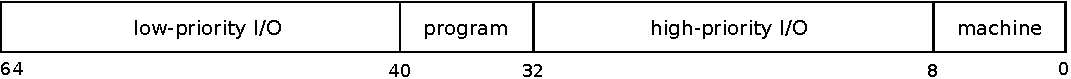
\includegraphics[width=\textwidth]{img/rKrQ-crop.pdf}
\end{figure}
\vspace{-20pt}
\noindent In general, the bits on the right have a higher priority than the bits on the left. Therefore, high-speed devices like network cards should get bits on the right, while slow devices like terminals should get bits on the left. But MMIX does not define the meanings of the I/O bits. Only the program (\glslink{Exception}{PEs}) and some of the machine bits (\glslink{Exception}{MEs}) are specified. The program bits are called {\tt rwxnkbsp} with the following meanings:
$$\vbox{\halign{{\tt #} bit: &#\hfil\cr
r	&	instruction tries to load from a page without read permission;\cr
w	&	instruction tries to store to a page without write permission;\cr
x	&	instruction appears in a page without execute permission;\cr
n	&	instruction refers to a privileged (negative) address;\cr
k	&	instruction is privileged, for use by the kernel only;\cr
b	&	instruction breaks the rules of\/ MMIX;\cr
s	&	instruction violates security (see below);\cr
p	&	instruction comes from a privileged address.\cr}}$$
The four specified machine bits from right to left stand for power failure, memory parity error, nonexistent memory and rebooting. MMIX defines, that the program bits have to be set in \sr{K} when executing in user mode (otherwise a security \glslink{Exception}{PE} is raised) and that program bit {\tt p} has to be zero in \sr{K} when executing in privileged mode (otherwise a privileged \glslink{Exception}{PE} is raised). \citep[pg. 29]{mmix-doc}

Analogous to the forced trip, the forced trap instruction is defined as:
\instrtblsix
	{\mi{TRAP X,Y,Z}}
	{$\sr{XX} \leftarrow 2^{63}~|$~\vmem{4}{@}}
	{$\sr{WW} \leftarrow @ + 4$}
	{$\sr{YY} \leftarrow \dr{Y},\quad \sr{ZZ} \leftarrow \dr{Z}$}
	{$\sr{BB} \leftarrow \dr{255},\quad \dr{255} \leftarrow \sr{J}$}
	{$\sr{K} \leftarrow 0$}
	{$@ \leftarrow \sr{T}$}
\noindent That means, besides the different handler location and the different set of special registers, \mi{TRIP} and \mi{TRAP} are equivalent, except that \mi{TRAP} clears \sr{K}. This way, dynamic traps are disabled. \citep[pg. 28]{mmix-doc} The operating system may even use instructions in a way that would raise a \glslink{Exception}{PE}, if the corresponding bit in \sr{K} were set. Because MMIX defines that "an instruction that traps with bits {\tt x}, {\tt k} or {\tt b} does nothing; a load instruction that traps with {\tt r} or {\tt n} loads zero; a store instruction that traps with any of {\tt rwxnkbsp} stores nothing" \citep[pg. 29]{mmix-doc}. The meaning of the operands {\tt X}, {\tt Y} and {\tt Z} can be defined by the operating system for any purpose. But two settings are predefined by MMIX:
\begin{enumerate}
	\item ${\tt XYZ} = 0$ should terminate the user process and
	\item ${\tt XYZ} = 1$ should offer a default action for a trip, for which the user program has not provided a handler (thus, instead of handling the trip, it can do a \mi{TRAP 0,0,1}).
\end{enumerate}

Analogous to forced and dynamic trips, the differences between forced and dynamic traps are, that for dynamic traps, the operands in \sr{YY} and \sr{ZZ} correspond to the operands of the interrupted instruction and the handler location is different. Additionally, MMIX defines that if "the interrupted instruction contributed 1s to any of the {\tt rwxnkbsp} bits of \sr{Q}, the corresponding bits are set to 1 also in \sr{XX}" \citep[pg. 29]{mmix-doc}. More precisely, these bits occur in the first byte of the upper tetra of \sr{XX}.

\subsection{Handling of Trips and Traps}

After having described the mechanisms of triggering trips and traps, it should be explained how they can be handled. This section starts with the instruction that resumes an interrupted computation, followed by the handling of trips and traps.

\subsubsection{Resuming}

Of course, MMIX has to be able to resume the ordinary execution after a trip or trap has been handled. To do so, it provides a quite sophisticated instruction that can be used for various purposes.

\instrtbleight
	{\mi{RESUME Z}}
	{if ${\tt Z} = 1$:}
	{$\quad \sr{K} \leftarrow \dr{255},\quad \dr{255} \leftarrow \sr{BB}$}
	{$@ \leftarrow \sr{W}|\sr{WW}$}
	{ropcode$~\leftarrow (\sr{X}|\sr{XX}) \gg 56$}
	{if ropcode$~= 0$: repeat(\sr{X}|\sr{XX})}
	{if ropcode$~= 1$: continue(\sr{X}|\sr{XX})}
	{if ropcode$~= 2$: set(\sr{X}|\sr{XX})}
	{if ${\tt Z} = 1~$and ropcode$~= 3$: trans(\sr{X}|\sr{XX})}
\noindent The instruction \mi{RESUME} comes in two versions: \mi{RESUME 0} resumes the computation after a trip, while \mi{RESUME 1} resumes it after a trap. Thus, \mi{RESUME 0} uses \sr{W} and \sr{X}, while \mi{RESUME 1} uses \sr{WW} and \sr{XX}. That does also mean, that the latter is prohibited in user mode. The default behaviour of \mi{RESUME}, when the so called \i{ropcode} is \haddr{80} (see \mi{TRIP} and \mi{TRAP}), is quite simple. The trip-version continues the execution at \sr{W}, while the trap-version sets \sr{K} and \dr{255} first and continues at \sr{WW} afterwards. But as the effect description shows, there are four other defined values of ropcode, which are more complicated. The four sketchy described actions have the following meaning:
\begin{itemize}
	\item repeat(\sr{X}|\sr{XX}):\\
	MMIX interprets the lower four bytes of \sr{X}|\sr{XX} as an instruction and executes it. This is allowed for all instructions except \mi{RESUME} itself.
	\item continue(\sr{X}|\sr{XX}):\\
	Continue is similar to repeat. It does also interpret the lower four bytes of \sr{X}|\sr{XX} as an instruction. But it does not use the operands provided in the instruction, but takes \sr{Y}|\sr{YY} and \sr{Z}|\sr{ZZ} instead. It is allowed for all "Set \dr{X} to the result of \dr{Y} OP \udrim{Z}" and "Set \dr{X} to the result of OP \udrim{Z}" instructions and for \mi{TRAP} as well. Some implementations of MMIX may also allow \mi{SYNCD} and \mi{SYNCID}. Another restriction is, that the instruction can not increase \sr{L}, \ie the {\tt X} operand of the instruction has to be less than \sr{L}.
	\item set(\sr{X}|\sr{XX}):\\
	This ropcode tells MMIX to set the register, denoted by the third least significant byte of \sr{X}|\sr{XX}, to \sr{Z}|\sr{ZZ}. Additionally, the third most significant byte is used to raise \glslink{Exception}{AEs}. Again, \sr{L} can not be increased.
	\item trans(\sr{X}|\sr{XX}):\\
	Last but not least, this ropcode can be used to put a translation into the translation cache. It uses \sr{YY} as the virtual address and \sr{ZZ} as the PTE and puts it into a TC. If the opcode of the instruction in the lower half of \sr{XX} is \mi{SWYM} (\i{sympathize with your machinery}; the NOP instruction of MMIX, that does nothing), the translation will be put into the instruction TC, otherwise in the data TC. Additionally, if this opcode is not \mi{SWYM}, the action repeat(\sr{XX}) will be performed.
\end{itemize}
All these actions behave as if they appeared as an instruction at location $\sr{W}|\sr{WW}-4$, \ie as if they have been inserted into the instruction stream at that position. \citep[pg. 30]{mmix-doc} It will be described shortly for what reasons the different actions, depending on ropcode, are offered.

\subsubsection{Handling Trips}

As said in the last section, all different kinds of trips have their own handler location, which are 16 bytes away from each other. That means, each handler has 4 instructions available to do what ever is necessary. For example, it could do something like:
\begin{center}
	\lstinline`PUSHJ $255,Handler; PUT rJ,$255; GET $255,rB; RESUME 0`
\end{center}
This way, the actual handler is called, saving all local registers on the stack. Before resuming, \sr{J} and \dr{255} have to be restored, because -- as described previously -- \mi{RESUME} will not do that. \citep[pg. 28]{mmix-doc}

Another way is to let the operating system perform the default actions for a trip by:
\begin{center}
	\lstinline`TRAP 0,0,1; GET $255,rB; RESUME 0`
\end{center}
In this case, no subroutine is called and thus, \sr{J} has not to be restored. \citep[pg. 28]{mmix-doc} Additionally, the reason why \mi{RESUME} does not restore the values saved by \mi{TRIP}, is that MMIX pursues the goal to perform only the minimum set of actions that are required.

When handling a dynamic trip, the operands of the instruction that caused the \glslink{Exception}{AE} are put into \sr{Y} and \sr{Z}. For example, if \mi{DIV \$0,\$1,0} is executed, MMIX will raise a division by zero \glslink{Exception}{AE} and set \sr{Y} to \$1 and \sr{Z} to 0. The handler could simply recognize that an \glslink{Exception}{AE} occurred. But it could also replace \sr{Y} and \sr{Z} with something else and change the ropcode in \sr{X} from \haddr{80} to \haddr{01} (continue). This way, the instruction would be repeated with operands \sr{Y} and \sr{Z}. Another way would be to set the ropcode to \haddr{02}, which would set \dr{X} to the value specified in \sr{Z}. \citep[pg. 28]{mmix-doc}

\subsubsection{Handling Traps}

Similarly to dynamic trips, dynamic traps that are triggered because of a \glslink{Exception}{PE}, save the operands of the instruction that caused it in \sr{YY} and \sr{ZZ}. MMIX does not define the meaning of these registers for all instructions. But it is defined that all "Set \dr{X} to the result of \dr{Y} OP \udrim{Z}" instructions put \dr{Y} in \sr{YY} and \udrim{Z} into \dr{Z}. Additionally, load instructions put the virtual address into \sr{YY}\footnote{Unfortunatly, the specification does not mention that explicitly for loads. But MMIX-PIPE does behave as explained and it would make no sense to do it for store instructions, but not for load instructions. After all, both may trigger a protection fault, for which the operating system has to know the virtual address. Having to calculate it from the {\tt Y} and {\tt Z} operand of the instruction for loads and simply read it from \sr{YY} for stores, would be very strange.}, while store instructions do additionally put the octa to be stored (including unchanged bytes for cases like \mi{STB}) into \sr{ZZ}. \citep[pg. 27]{mmix-doc}

Additionally it is noteworthy, that the OS has not many choices when considering \glslink{Exception}{PE} handling. Because the only \glslink{Exception}{PEs}, which are well defined, are the protection faults. For all others, \ie when refering to a negative address, using a privileged instruction, breaking the rules of MMIX, violating security or jumping to a privileged address, the MMIX specification does not define the values of \sr{WW} and \sr{XX}. Thus, the operating system is unable to resume the computation of the user program in a reliable way. But of course, these \glslink{Exception}{PEs} indicate a malicious or faulty user program anyway, so that the best option is a kill (and perhaps providing feedback to the user in form of a log entry or similar).

MMIX does also allow cheaper implementations of it, that let the software realize some instructions. In this case, these instructions cause a forced trap. For example, expensive operations like \mi{DIV} or \mi{FREM} could be implemented in software by checking the opcode in \sr{XX} when handling a forced trap. If it is one of these instructions, the result will be computed, put into \sr{ZZ} and the ropcode will be set to \haddr{02}. A subsequent \mi{RESUME 1} will place \sr{ZZ} into the desired register. As already said, even arithmetic \glslink{Exception}{exceptions} could be raised by specifying them in the third most significant byte of \sr{XX}. \citep[pg. 28]{mmix-doc}

A similar feature is, that address translation can be done in software. This can be requested by setting field $f$ of \sr{V} to 1, but some implementations of MMIX might even require that. As soon as a translation is necessary, \ie it is not already in the corresponding TC, a forced trap with ropcode \haddr{03} is triggered. The virtual address will be available in \sr{YY}. When the translation is done, the handler should put the physical address into \sr{ZZ}. A subsequent \mi{RESUME 1} will put this translation into the TC and repeat the instruction, which will succeed this time. It should be noted, that if an instruction fetch fails, MMIX will put the instruction \mi{SWYM} into \sr{XX}. This way, the translation will be put into the instruction TC and the fetch will be repeated when \mi{RESUME 1} is executed. \citep[pg. 28]{mmix-doc}

\subsection{Interruptibility}
\label{sec:mmix-interruptibility}

Because of the complexity of some instructions (like \mi{SAVE}, \mi{POP}, \mi{DIV}, \mi{FREM} and so on), MMIX allows them to be interruptible. The specification words it as:
\begin{quote}
Non-catastrophic \glslink{Interrupt}{interrupts} in MMIX are always precise, in the sense that all legal instructions before a certain point have effectively been executed, and no instructions after that point have yet been executed. The current instruction, which may or may not have been completed at the time of \glslink{Interrupt}{interrupt} and which may or may not need to be resumed after the \glslink{Interrupt}{interrupt} has been serviced, is put into the special execution register \sr{X}, and its operands (if any) are placed in special registers \sr{Y} and \sr{Z}.\footnote{Actually, \sr{XX}, \sr{YY} and \sr{ZZ} are meant (which were introduced later in the specification), because the other ones are only used for trips, which are either explicitly requested or raised for \glslink{Exception}{AEs}. Thus, they do not occur at arbitrary points of time during a computation, as \glslink{Interrupt}{interrupts} from I/O devices may.} \citep[pg. 27]{mmix-doc}
\end{quote}
That means, if an \glslink{Interrupt}{interrupt} occurs while executing an instruction, a particular MMIX implementation may wait briefly until an interruption is possible and then put the state of computation of the current instruction into \sr{XX}, \sr{YY} and \sr{ZZ}. In this case, the meaning of the registers is completely implementation dependent. For example, \mi{FREM \$X,\$Y,\$Z} may set \sr{YY} and \sr{ZZ}, such that $\sr{YY} \bmod \sr{ZZ} = \dr{Y} \bmod \dr{Z}$, but the actual values of \sr{YY} and \sr{ZZ} may be different than \dr{Y} and \dr{Z}. \citep[pg. 27 and 29]{mmix-doc} If MMIX sets ropcode to \haddr{01} (continue), the operating system will not be required to care about that, because a \mi{RESUME 1} will simply execute that instruction again with \sr{YY} and \sr{ZZ}, which will lead to the same result.

It should also be mentioned, that \sr{XX} might not hold the instruction found at address $\sr{WW}-4$. Not only because of jumps, but also because MMIX might put an instruction into \sr{XX}, that has been inserted internally. For example, if \mi{ADD \$X,\$Y,\$Z} is executed with ${\tt X} \ge \sr{L}$, the hardware may insert an instruction to increase \sr{L} first.




\chapter{The Implementation of GIMMIX}

Now that the entire MMIX architecture has been explained, the simulator GIMMIX should be described in detail. As already mentioned in the introduction, GIMMIX has been developed with the goal to be able to port an operating system to it. Therefore GIMMIX pursues to be correct (which implies to be not more complex than necessary), implement MMIX completely and offer a convenient and productive user interface, so that an OS can be debugged.

This chapter splits the depiction of GIMMIX into five parts. At first, the design decisions for the implementation are explained, followed by an overview of the simulator. Subsequently, the implementation of the MMIX architecture (the "core") is described in detail and yet existing devices are introduced shortly. Finally, the command line interface (CLI), which allows it to debug an OS or arbitrary other programs for MMIX, is presented.

\section{Basic Design Decisions}

Before starting with the description of the simulator, a few general design decisions that have been made should be explained.

\subsection{No Pipelining}

At first, it has been decided to abandon \glslink{Pipelining}{pipelining}. Since it is a simulator, \ie implemented in software, and has not the goal to explore the difficulties for a potential hardware \glslink{Pipelining}{pipelining} implementation or similar, using \glslink{Pipelining}{pipelining} would not bring advantages. Without it, the simulator is much simpler and thus the correctness is easier to achieve.

\subsection{Uninterruptible Instructions}

Similarly to the previous one and a bit related to it, it has been decided to make instructions uninterruptible, \ie an instruction is either executed completely or not at all, as far as no \glslink{Exception}{program or machine exception} occurs. As mentioned in \ref{sec:mmix-interruptibility} of chapter \ref{ch:mmix-arch}, MMIX allows it to make complex instructions like \mi{POP} or \mi{SAVE} interruptible by encoding the current state of computation in \sr{XX}, \sr{YY} and \sr{ZZ}. But it does not require implementations to do that, which means that it is specification conform to make all instructions uninterruptible. \citep[pg. 27]{mmix-doc}

Without this decision, GIMMIX would have required a concept that allows it to execute instructions in multiple steps, pause them for \glslink{Interrupt}{interrupts} and resume them later. This would have made it a lot more complex, without leading to real advantages for similar reasons as in the previous decision. Thus, for simplicity all instructions in GIMMIX are uninterruptible.

\subsection{Programming Language}

Obviously, when one wants to run an operating system in a simulator, \ie a program that implements the whole simulated machine in software, efficiency is very important. Additionally, a lot of control over the produced machine code is necessary to be able to imitate the exact behaviour of the simulated machine. Therefore it has been decided to use the programming language C, which both allows to build efficient programs and offers a lot of control. Additionally, MMIX-SIM and MMIX-PIPE are implemented in C as well\footnote{As mentioned, they are written with CWEB, which produces C code in the end.}, so that it is easier to use code from them, such as the floating point algorithms.

Since an octa is the word quantity of MMIX, it will be used at nearly all places in the simulator. Therefore, its representation affects more or less the whole code. Using \glslink{C89C99}{C89} on a 32-bit platform would mean, that no 64-bit type is available \citep{llgccext}. Thus, a struct would have to be created, that contains two 32-bit integers; one for the upper half of the octa and one for the lower half. Of course, every operation that is done with an octa, would have to be broken down to operations with the two 32-bit integers. In other words, the whole code of the simulator would get a lot more difficult to read and write, just because of the fact that there is no 64-bit type.

But there is an alternative. \glslink{C89C99}{C99} provides the so called \i{exact-width integer type} `uint64_t`, which does always correspond to an unsigned 64-bit integer, independent of the underlying platform \citep{uint64t}. That is, the compiler will arrange things, such that this type (including all possible operations with it) is available. Although most currently available compilers offer no complete implementation of \glslink{C89C99}{C99} yet \citep{c99supp}, even the old version 3.0 (released 2001 \citep{gccrel}) of the GNU C Compiler, which is used in this project, supports this feature including many other useful ones \citep{gcc30c99}. For these reasons, \glslink{C89C99}{C99} has been selected, but GIMMIX will only utilize some basic features of it such as exact-width integer types, "`//` comments", mixed declarations and code, initialization in for-loops and `snprintf`, which are available in \gls{gcc} and should be in almost all other compilers as well.

\subsection{Host Platform}

The host platform, \ie the platform that runs the simulator, is expected to be a Linux system. Although most parts of GIMMIX are platform independent, some of them -- like the simulated terminals for example -- assume Linux. Furthermore, the simulator core (excluding \eg some test generation programs, that expect x86) uses only standard \glslink{C89C99}{C99}, which means it should be hardware independent (but it has not been tested with different hardware).

Since both 32 and 64-bit platforms are widely spread nowadays, GIMMIX has the effort to support both of them. This is mostly achieved behind the scenes by adding a layer on top of the `printf`, `scanf` and `strtol` families. For the first two families, the layer lets the user specify the size of an argument with 'O','T','W' or 'B' (additionally to 'h', 'l' and 'L') for octa, tetra, wyde or byte, respectively. For `strtol`, the layer calls simply either `strtol` or `strtoll`, depending on the platform. But there are a few other things to take care of. For example, when using logical or arithmetical negation, the result depends on the size of the operand. That means, \eg `-sizeof(octa)` could lead to different results. If the type of `sizeof(octa)` is 32 bit wyde, the logical negation would produce \haddrt{FFFF}{FFF8}, instead of the perhaps intended \haddro{FFFF}{FFFF}{FFFF}{FFF8}. Thus, whenever such operators are used with this intention, the operand has to be casted to an octa first.


\section{Overview}

Before explaining the main parts of GIMMIX, this section gives an overview and introduces the basic components, that are used throughout the code.

Conceptually, GIMMIX consists of several \i{modules} that interact with each other. The name of a module corresponds to a source file or folder in the directory \file{src} and to the associated header file or folder in the directory \file{include}. The following \gls{FMC} diagram illustrates the most important modules and their relationships, whereas the CLI, the core and the devices are only shown as black boxes for now:
\begin{figure}[H]
	\centering
	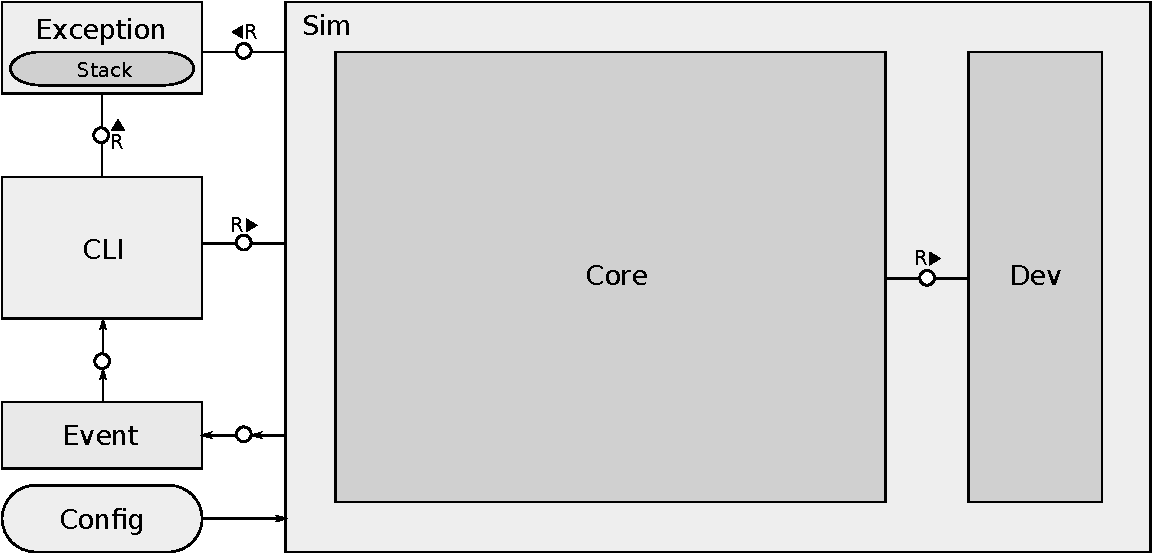
\includegraphics[width=\textwidth]{img/sim-fmc-crop.pdf}
	\caption{Architecture of GIMMIX in \protect\gls{FMC} notation}
	\label{fig:gimmix-arch}
\end{figure}
\noindent That means, the modules \i{core} and \i{dev}, to which the core sends requests for tasks like reading an octa from a specific physical address, are in a sense enveloped in \i{sim}. Sim supports some basic operations like initializing the whole system, resetting it or shutting it down. This is controlled by the module \i{CLI} (when running in interactive mode). The following sections describe the other general modules in the figure.

\subsection{Exception}

Although \glslink{Exception}{exception} handling in C via `setjmp` and `longjmp` is not as convenient and powerful as for example in Java, it offers some advantages. That is, it separates "normal" code from exceptional code and provides the possibility to handle an \glslink{Exception}{exception} only at places, where it can be handled in a sensible way. To achieve that and allow nested "try and catches", the module \i{exception} manages a stack of `jmp_buf`s, which hold the state created by `setjmp`. It is used for trips and traps in the core and also for \glslink{Exception}{exceptions} in the CLI. The most important functions are:
\begin{itemize}
	\item `ex_push(jmp_buf *environment)`:\\
	This function pushes the given environment onto the stack and is thus the equivalent to a `try`. The environment \i{has to} be created by the caller, because one can not jump back to a stack frame, that has been already destroyed.
	\item `ex_throw(int exception,octa bits)`:\\
	As the name suggests, it throws the \glslink{Exception}{exception} with given number and additional information in `bits`, which is used for example to specify what trip or trap should be triggered. That is, it calls `longjmp` with the topmost `jmpbuf` and `exception` as arguments, so that the caller of `setjmp` receives `exception` as return-value.
	\item `ex_pop()`:\\
	This function removes the topmost environment from the stack. Hence, it is the equivalent to the end of a try-catch-construct.
\end{itemize}
In this thesis, the term "\glslink{Exception}{exception}" without the prefix "arithmetical", "program" or "machine", refers to this concept, instead of the different \glslink{Exception}{exceptions} of MMIX.

\subsection{Event}

As already mentioned, GIMMIX offers a sophisticated CLI that should allow it to debug an operating system or other programs in a convenient way. To do so, the CLI needs of course access to the core, \ie it has to read the current state and should also be able to display the effect of an instruction or set breakpoints. Integrating all those facilities into the core would mean, that it gets more difficult to read and understand and it would also introduce strong coupling between the CLI and the core. Since the core is quite stable (the architecture is not expected to change much), but it may indeed be imaginable to provide a graphical user interface (GUI) to GIMMIX some day, it has been decided to work with events to supply the user interface with information. This way, the core is completely independent of the CLI and thus, assuming that a GUI is ready, it could replace the CLI within minutes, without affecting the core.

The module \i{event} implements this idea by providing `ev_register` to register a callback function for a specific event and `ev_unregister` to unregister it again. Additionally, events can be fired by calling `ev_fire`, `ev_fire1` or `ev_fire2` to raise an event with 0, 1 or 2 arguments, respectively. As figure \ref{fig:gimmix-arch} suggests, the core fires events and the event module forwards them to the CLI (and any other interested modules), which has registered the corresponding callbacks at the beginning. It is noteworthy, that if GIMMIX is used in non-interactive mode, the CLI will not be used at all and thus no callback will be registered, which will allow GIMMIX to be as performant as possible.

\subsection{Config}

Of course, GIMMIX should be configurable to some extent, which is realized by the module \i{config}. It consists of two categories of settings: the settings in the first one are configurable during compile time (\ie constants are used) and the other ones are configurable during runtime. The latter can be passed to GIMMIX as command line arguments. In a sense, the compile time options are those that would be fixed when GIMMIX were a solid piece of hardware (number of local registers, cache size, device addresses, \dots), while the runtime options could be changed more easily (amount of main memory, number of terminals, disk image, \dots). But of course, there are also practical reasons, why one has to be able to specify the disk image or the rom image via command line argument.


\section{Simulator Core}

This section describes the most important part of the simulator, \ie the implementation of the MMIX architecture.

\subsection{Structure}

The following figure breaks the core, that has been displayed as a black box in the previous \gls{FMC} diagram, further down into pieces:
\begin{figure}[H]
	\centering
	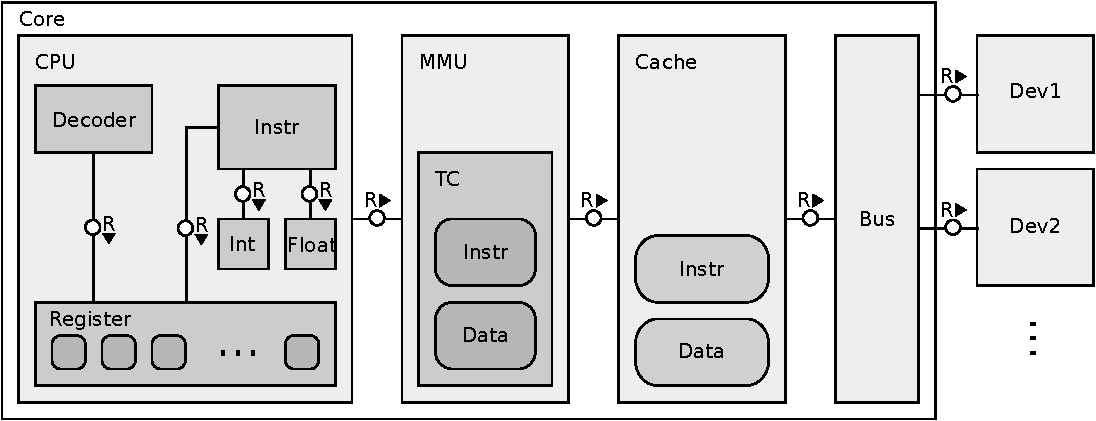
\includegraphics[width=\textwidth]{img/sim-core-fmc-crop.pdf}
	\caption{Architecture of the core in \protect\gls{FMC} notation}
\end{figure}
\noindent That means, it consists of four parts: \i{CPU}, \i{MMU}, \i{cache} and \i{bus}, whereas requests are always done from left to right. For example, when using \mi{LDO} to read an octa from main memory (RAM, which is a device as well), the load instruction will request it from the MMU, which might have to translate the virtual address to a physical one first. Subsequently, the MMU will send a request to the cache to read an octa from the obtained physical address. If it is not in the data cache yet, the cache will send a request to the bus, which in turn will find the associated device and forward the request to it. Finally, the RAM device reads the octa from main memory and the result is passed back, ending at the load instruction.

The CPU consists of several parts as well. It has a module named \i{decoder}, which obviously is responsible for decoding an instruction. Additionally, the module \i{instr} implements all MMIX instructions, using \i{int} and \i{float} for integer and floating point arithmetic, respectively. Finally, the module \i{register} realizes the register stack.

The different parts shown in the diagram are explained in more detail in the following sections.

\subsection{CPU}

As the name suggests, the CPU is the central unit in GIMMIX, that is responsible for executing the instructions, using the help of several other modules.

\subsubsection{Executing an Instruction}

The execution of instructions is separated into three phases:
\begin{enumerate}
	\item fetching the instruction, \ie loading the tetra from memory,
	\item decoding the instruction, which means that the operands are extracted from the tetra and translated into \i{arguments}, depending on the opcode and
	\item executing the instruction, taking the arguments and performing the required actions.
\end{enumerate}
The code in module CPU, that realizes the described procedure, looks like the following:
\begin{lstlisting}[language=C,caption=Executing an instruction (slightly shortened)]
jmp_buf env;
int ex = setjmp(env);
if(ex != EX_NONE)
	cpu_triggerException(ex,ex_getBits());
else {
	ex_push(&env);

	// fetch instruction
	ev_fire(EV_BEFORE_FETCH);
	instrRaw = mmu_readInstr(pc,MEM_SIDE_EFFECTS);

	// decode
	instr = dec_getInstr(OPCODE(instrRaw));
	cpu_checkSecurity();
	dec_decode(instrRaw,&iargs);

	// execute
	ev_fire(EV_BEFORE_EXEC);
	instr->execute(&iargs);

	// handle realtime tasks
	if(++instrCount == INSTRS_PER_TICK) {
		instrCount = 0;
		timer_tick();
	}
	cpu_checkForInterrupt();
	cpu_counterTick();
}
ex_pop();
ev_fire(EV_AFTER_EXEC);
pc += sizeof(tetra);
\end{lstlisting}
As the listing shows, the whole procedure is surrounded by a kind of try-catch-construct, because several parts of it may throw an \glslink{Exception}{exception}. If an \glslink{Exception}{exception} is thrown, it will jump back to the `setjmp` call, which will return the \glslink{Exception}{exception}-number. Afterwards the requested trip or trap is triggered (this will be described in detail later). Additionally, the code fires events at several interesting places to allow the CLI to perform some actions. After the instruction has been executed, realtime tasks are done if necessary (which might result in a finished disk-command or similar), it is checked whether $\sr{Q}\land\sr{K}$ is non-zero and the counters are ticked (\sr{C}, \sr{U} and \sr{I}). Finally, the \gls{PC} is advanced to the next instruction. It should be mentioned, that the function `cpu_checkSecurity` ensures that all program bits are set in \sr{K}, when running in user mode, and that the privileged \gls{PC} bit is \i{not} set, when running in privileged mode.

The actual decoding is done by the function `dev_decode` of the module \i{decoder}. The decoder contains a table, that assigns to each instruction both an \i{instruction format} and \i{argument format}. The first one defines the meaning of the three operand bytes `X`, `Y` and `Z`. The second defines the arguments for the execution-function. More precisely, those functions receive a struct that contains the fields `x`, `y` and `z`, but the meaning of the fields differs, depending on the argument format. For example:
\begin{itemize}
	\item \mi{ADD} (`I_RRR`, `A_DSS`): ${\tt x}={\tt X}$, ${\tt y}=\dr{Y}$, ${\tt z}=\dr{Z}$
	\item \mi{ADDI} (`I_RRI8`, `A_DSS`): ${\tt x}={\tt X}$, ${\tt y}=\dr{Y}$, ${\tt z}={\tt Z}$
	\item \mi{BNN} (`I_RF16`, `A_CT`): ${\tt x}=\dr{X}$, ${\tt z}=@ + 4*{\tt YZ}$
	\item \mi{STBI} (`I_RRI8`, `A_SA`): ${\tt x}=\dr{X}$, ${\tt y}=\dr{Y} + {\tt Z}$
\end{itemize}
In other words, the decoder performs a mapping from the instruction operands to the arguments, which hide certain details from the execution function. For example, the functions that implement the branches will simply receive the address to jump to and do not have to care about jumping forward or backwards and so on. Similarly, instructions like \mi{ADD} and \mi{ADDI} are put together, \ie there is only one execution function for both, because the differences are handled by the decoder.

Besides the fact that the separation of decoding and executing prevents code duplication and is arguably more elegant, there is also a technical reason for it. Because, as described in the previous chapter, the instruction \mi{RESUME} has a ropcode that allows it to execute the typical "set `X` to the result of `Y` OP `Z`" instructions and some other, whereas the operands are taken from \sr{YY} and \sr{ZZ} instead of from the instruction itself. Thus, many instructions need to be executable both in the ordinary and in this special way. Since this separation hides the origins of the operands from the execution function, this is no problem anymore, because when implementing \mi{RESUME}, one can simply create the argument struct from the instruction in \sr{XX} and exchange `y` and `z` with \sr{YY} and \sr{ZZ}, respectively.

\subsubsection{Execution Functions}

The execution functions, mentioned in the previous section, are in most cases very short and simple. Because the arguments are provided in the desired form from the decoder and because other modules like MMU, int, float and register do the hard work. The following listing shows a few examples:
\begin{lstlisting}[language=C,caption=Examples of the execution functions]
void cpu_instr_nor(const sInstrArgs *iargs) {
	octa res = ~(iargs->y | iargs->z);
	reg_set(iargs->x,res);
}

void cpu_instr_stou(const sInstrArgs *iargs) {
	mmu_writeOcta(iargs->y,iargs->x,MEM_SIDE_EFFECTS);
}

void cpu_instr_bev(const sInstrArgs *iargs) {
	if(!(iargs->x & 1))
		jumpTo(iargs->z);
}
static void jumpTo(octa addr) {
	if(!cpu_isPCOk(addr))
		ex_throw(EX_DYNAMIC_TRAP,TRAP_PRIVILEGED_PC);
	// substract sizeof(tetra) because it will be increased
	cpu_setPC(addr - sizeof(tetra));
}
\end{lstlisting}
That means, the implementation of \mi{NOR} simply performs the bit operation and sets \dr{X}, \mi{STOU} uses `mmu_writeOcta` to write `iargs->x` to `iargs->y` and \mi{BEV} jumps to the desired location if `iargs->x` is even. The latter has to check the \gls{PC} first to make sure that no jump from user space to privileged space can be done.

Besides this simplicity, there is an important point every instruction has to take care of. Although all instructions are uninterruptable, \ie an \glslink{Interrupt}{interrupt} can not happen during their execution, of course program \glslink{Exception}{exceptions} can occur. Thus, every execution function (and many other functions as well) has to pay attention to this. In most cases, as in `cpu_instr_stou` above, it is simple because there is at most one function, that might throw an \glslink{Exception}{exception}. Therefore, calling this function at first, \ie before the state has changed, solves the problem. But if multiple functions might throw an \glslink{Exception}{exception}, it gets more complicated:
\begin{lstlisting}[language=C,numbers=left,numberstyle=\footnotesize,caption=Execution function of \mi{CSWAP}]
void cpu_instr_cswap(const sInstrArgs *iargs) {
	octa addr = iargs->y + iargs->z;
	octa mem = mmu_readOcta(addr,MEM_SIDE_EFFECTS);
	if(mem == reg_getSpecial(rP)) {
		octa val = reg_get(iargs->x);
		reg_set(iargs->x,0);
		reg_set(iargs->x,val);
		mmu_writeOcta(addr,val,MEM_SIDE_EFFECTS);
		reg_set(iargs->x,1);
	}
	else {
		reg_set(iargs->x,0);
		reg_setSpecial(rP,mem);
	}
}
\end{lstlisting}
In this case, the functions to be careful with are `mmu_readOcta`, `reg_set` (storing values on the stack might lead to an \glslink{Exception}{exception}) and `mmu_writeOcta`. Obviously, if multiple functions change the state and might throw an \glslink{Exception}{exception}, calling them at first will not work. The following trick does solve the problem for \mi{CSWAP}. The read in line 3 does not change the state (caches are not considered critical in this case) and can thus be called at first. The `reg_set` in line 6 sets \dr{X} to an arbitrary value. If this function throws, nothing will have been changed yet. If it does not, line 7 will set \dr{X} back to the original value, which can not throw because the previous `reg_set` would have already done that. Hence, if the write in line 8 throws, the state will not have been changed yet. If line 9 is reached, `reg_set` will not throw either. All in all, no matter which function throws, the state has not changed (line 12 is not critical here). Additionally, all used functions are assumed to be \glslink{Exception}{exception}-safe as well. It will be described later, that a few functions actually do not garantee to be atomic, \ie do not change the state if an \glslink{Exception}{exception} occurs, but only make sure that a consistent state is reached.

\subsubsection{Arithmetic}

As described, MMIX supports both integer and floating point arithmetic. GIMMIX uses the modules \i{int} for integer arithmetic and \i{float} for floating point arithmetic. The former only implements the operations that differ from the behaviour defined by \glslink{C89C99}{C99}. The latter handles all operations in software, \ie uses the integer arithmetic of the underlying platform. Both -- and especially float -- contain very complicated algorithms, but because they are not the central points of this thesis, they are described only sketchy. Besides that, they have been inherited from MMIX-SIM/MMIX-PIPE and have only been adjusted for GIMMIX. All functions are implemented, so that they are independent of the rest of the simulator. That means, they do not access registers, change the state or similar.

\paragraph{Integer Arithmetic}

The module int contains functions for 128-bit signed and unsigned multiplication and division. They basically break down the operation to the 16-bit or 32-bit multiplication or division of the underlying platform, because 128-bit versions are not available. Additionally, the division has to handle the differences to \glslink{C89C99}{C99}. Because MMIX requires floored division, while \glslink{C89C99}{C99} defines that truncated division is used \citep[pg. 82]{c99std}. Additionally it is worth mentioning, that the signed versions of both multiplication and division are based on the unsigned versions and only adjust the result accordingly.

The three shift types of MMIX -- shift left, shift right arithmetically and shift right logically -- are implemented in this module as well. The reason is, that \glslink{C89C99}{C99} says:
\begin{quote}
If the value of the right operand is negative or is greater than or equal to the width of the promoted left operand, the behavior is undefined. \citep[pg. 84]{c99std}
\end{quote}
Thus, the functions implementing the shifts ensure, that for example $1 \ll 65$ leads to zero, as MMIX defines it.\footnote{For example, the result of $1 \ll 65$ with \gls{gcc} 4.4.5 on x86\_64 is 2 instead of 0, because $x \ll y$ does actually mean $x \ll (y \bmod (sizeof(y)*8))$.}

\paragraph{Floating Point Arithmetic}

The basic principle in module float is to use the function `fl_unpack` to extract the components of a float from an octa. It returns a structure called `sFloat`, that contains the sign, the exponent, the fraction and the type (`ZERO`, `NAN`, `INF` or `NUM`). If the number is denormalized, it will be normalized and the exponent gets negative to abstract away the differences. Additionally, the fraction is always shifted left by 2, leading to two zero bits at the end, that are used for rounding and detection of inexact results.

All floating point operations work with instances of `sFloat`. Most of them consist of a `switch`, that does the corresponding action or returns the corresponding value, depending on the type of the operand(s). Finally, `fl_pack` is used to build an octa from the `sFloat` structure, which has represented the result so far. Consequently, it goes the opposite way than `fl_unpack`. It also rounds the result with the requested rounding mode and indicates overflow, underflow and inexact \glslink{Exception}{AEs}, if necessary. These are not directly triggered, but passed back to the caller. As soon as short floats are used, `fl_spack` and `fl_sunpack` are chosen instead of `fl_pack` and `fl_unpack`.

\subsubsection{Register}

The module \i{register} is one of the most important and also most complicated ones. Therefore, this thesis describes it in depth. Obviously, it is responsible for managing the registers. Additionally, it implements the main parts of the instructions \mi{PUSHJ}, \mi{PUSHGO}, \mi{POP}, \mi{SAVE} and \mi{UNSAVE}. More precisely, the parts that affect the register stack. Thus, checking the instruction operands, setting the new \gls{PC} and similar tasks, are done by the execution function, while the rest is done by the register module.

\paragraph{Basic Data Structures and Operations}

The basic data structures and functions of register are quite simple. It has the arrays `local`, `global` and `special` to hold local, global and special registers, respectively. Furthermore, it manages the abbreviations `L` for \sr{L}, `G` for \sr{G}, `S` for $\sr{S}/8$ and `O` for $\sr{O}/8$. The last two are used as indices into `local` and -- instead of what the description of MMIX said -- modulo is not used all the time (\ie in general, ${\tt O} \ne (\sr{O}/8) \land (2^n-1)$), but only if `local` is accessed. In code listings, $2^n-1$ will be called `LREG_MASK`, analogously to `GREG_MASK` for the global registers.

To offer other modules access to the mentioned arrays, the following functions are provided:
\begin{itemize}
	\item `reg_getLocal`/`reg_setLocal`:\\
	These functions return or set the value of the specified local register, independent of `O`. This is not used by the core, but only by the CLI at the moment.
	\item `reg_getGlobal`/`reg_setGlobal`:\\
	These ones return or set the value of the specified global register and are also only used by the CLI.
	\item `reg_getSpecial`/`reg_setSpecial`:\\
	Similarly, these functions return or set the value of the specified special register.
	\item `reg_get`/`reg_set`:\\
	Finally, these two return or set the value of the specified dynamic register, \ie if `rno` is the desired register number, ${\tt rno} \ge {\tt G}$ will denote global register `rno`, ${\tt rno} < {\tt L}$ will denote local register $({\tt O}+{\tt rno}) \land (2^n-1)$ and other values denote marginals.
\end{itemize}
The most interesting function just described, is `reg_set`, which is implemented as follows:
\begin{lstlisting}[language=C,caption=Implementation of {\tt reg\_set}]
void reg_set(int rno,octa value) {
	if(rno >= G)
		global[rno & GREG_MASK] = value;
	else {
		while(rno >= L) {
			local[(O + L) & LREG_MASK] = 0;
			if(((S - O - (L + 1)) & LREG_MASK) == 0)
				reg_stackStore();
			special[rL] = L = L + 1;
		}
		local[(O + rno) & LREG_MASK] = value;
	}
}
\end{lstlisting}
As the listing shows, if `rno` is greater than or equal to `L`, `L` will be increased first and registers will be set to zero. If the registerring is full, \ie if the number of used local registers (plus one to leave a slot free) is equal to the number of available slots (difference of `S` and `O`), a register will have to be written to memory first. More precisely, `reg_stackStore` writes `local[S & LREG_MASK]` to \vmem{8}{\sr{S}} and increases \sr{S} by 8 and `S` by 1.

Similarly to the implementation of \mi{CSWAP}, `reg_set` has to take care of \glslink{Exception}{exceptions}, that might be thrown when writing to memory. But in contrary to \mi{CSWAP}, it does not ensure that the state does not change. Instead, it will always leave in a consistent state. That means, if `reg_stackStore` fires an \glslink{Exception}{exception}, the function might have already increased `L` and cleared some registers. But it is no problem, because the state is ok and the repetition of the instruction will continue at the point just left. To allow that, it is important that the increasing of `L` is done \i{after} storing a value on the stack. Doing it in the other way around would lead to an inconsistent state.

\paragraph{Pushing Registers Down}

The function, that performs the central tasks of \mi{PUSHJ} and \mi{PUSHGO} is called `reg_push` and receives the `X` operand of the instruction as argument. It is implemented in the following way:
\begin{lstlisting}[language=C,caption=Implementation of {\tt reg\_push}]
void reg_push(int rno) {
	int curL = L;
	if(rno >= G) {
		rno = curL++;
		if(((S - O - curL) & LREG_MASK) == 0)
			reg_stackStore();
		local[(O + rno) & LREG_MASK] = rno;	// set hole
	}
	else {
		reg_set(rno,rno);	// set hole
		curL = L;
	}

	O += rno + 1;			// push down
	special[rO] += (rno + 1) * sizeof(octa);
	L = curL - (rno + 1);	// move L down (keep arguments)
	special[rL] = L;
}
\end{lstlisting}
That means, at first the hole is set to `rno` to remember the number of pushed down registers. Afterwards, `O` is increased correspondingly and `L` is adjusted, so that the arguments for the callee are kept. If ${\tt rno} \ge {\tt G}$, `rno` will be set to `L`, `L` will be increased by 1 and a register might have to be written to memory first. Similarly to `reg_set`, the function has to take care of the \glslink{Exception}{exceptions} thrown by `reg_stackStore`. Thus, `L` is not changed before the call to ensure that the state has not been changed if it throws.

\paragraph{Popping Registers}

The implementation for \mi{POP}, which receives the number of registers to return as argument, is a bit more complicated:
\begin{lstlisting}[language=C,caption=Implementation of {\tt reg\_pop}]
void reg_pop(int rno) {
	octa holeData;		// last return value -> hole
	if(rno != 0 && rno <= L)
		holeData = local[(O + rno - 1) & LREG_MASK];
	else
		holeData = 0;	// if rno > L, hole <- 0

	int numRets = rno <= L ? rno : L + 1;
	if(special[rS] == special[rO]) {
		reg_stackLoad();
		if(((S - O - L) & LREG_MASK) == 0)
			special[rL] = --L;
	}
	int numRegs = local[(O - 1) & LREG_MASK] & 0xFF;
	
	while((tetra)(O - S) <= (tetra)numRegs) {
		reg_stackLoad();
		if(((S - O - L) & LREG_MASK) == 0)
			special[rL] = --L;
	}

	L = numRegs + numRets;
	if(L > G)
		L = G;
	// set hole
	if(L > numRegs)
		local[(O - 1) & LREG_MASK] = holeData;
	O -= numRegs + 1;
	special[rO] -= (numRegs + 1) * sizeof(octa);
	special[rL] = L;
}
\end{lstlisting}
At first, the value for the hole is calculated. If ${\tt rno} \le {\tt L}$, it will be set to the last return value, if ${\tt rno} > {\tt L}$, it will be set to zero and if ${\tt rno} = 0$, the hole will not be set at all. Afterwards, the number of local registers the caller wanted to keep, is determined. It might be necessary to load this value back from memory into a register first. Subsequently, if required, local registers will be restored until the desired `numRegs` are available. Finally, `L` is set for the caller, the hole is written and `O` is decreased correspondingly.

Again, \glslink{Exception}{exception}-safety has to be considered. Of course, both calls of `reg_stackLoad` might throw an \glslink{Exception}{exception}. At a first glance one might think that it is sufficient to make sure, that all instructions can be repeated successfully, after the \glslink{Exception}{PE} that they had triggered previously, has been handled. In this case it would mean, that we do not need to care about it, because only a few registers of the caller might have been already loaded and will not be loaded again when repeating the instruction. But unfortunatly this is not enough. Because the OS might choose not to repeat the function directly, but \eg let the user application handle a signal first (or something else, that is asynchronous to the ordinary control flow)\footnote{At least, the MMIX specification does not say the opposite. Therefore it is considered valid to let the user application handle a signal first when leaving the kernel, even if the kernel has been entered because of a \glslink{Exception}{PE}.}. In this case, arbitrary other instructions may be used and thus, the state of MMIX and in particular the state of the register stack has to be consistent. To ensure it in `reg_pop`, `L` has to be decreased when a register is restored. This way, one register of the callee is exchanged for a register of the caller. If this was not been done, the condition that $\alpha$, $\beta$ and $\gamma$ may never move past each other, would be violated.

\paragraph{Page Faults on the Stack}

Unfortunatly, the current version of the MMIX architecture, described in this thesis, has a design flaw. Because if a process causes a page fault while accessing the stack (for example, when using \mi{PUSHJ}, \mi{POP}, \mi{SAVE} or setting a register), the operating system will not be able to save the state, handle the \glslink{Exception}{PE} and resume the process successfully. Because obviously, the OS needs at least a few registers to be able to handle a \glslink{Exception}{PE}. But in general (\ie if the OS does not define, that some global registers can not be used by user applications), no register is available. Thus, the OS has to save a few registers first. For example, \mi{SAVE} could be used for that purpose to save the whole state of the running program. But \mi{SAVE} will write the state onto the stack, which does of course not work, because the stack has caused the page fault. Using \mi{PUSHJ} to push some registers down would be an alternative way to supply the OS with a few registers. But equally, \mi{PUSHJ} might have to save registers on the stack. Additionally it is not possible to save the state manually, because at least one register has to be available to build the destination memory address. In sum, there is no way to save the state of the running program. The consequence is, that the OS has either to restrict the user applications to dedicate some global registers to the OS, or it has to assign a stack of constant size, that is not swapped out or similar, to the applications.

Since these restrictions are not acceptable, it has been chosen to solve this problem. The basic idea is to give the operating system a different stack than the user applications. To do so, a new special register called \sr{SS} is introduced, which holds the desired address of the \i{kernel stack}. Additionally, \mi{SAVE} and \mi{UNSAVE} are extended to offer a second version, which switches to the kernel stack and back to the user stack, respectively. That means, that \mi{SAVE} will first set \sr{S} to \sr{SS} and will save the whole state on this stack. Consequently, \mi{UNSAVE} will do the opposite, \ie it first loads all values from the kernel stack back into registers and then will switch back to the user stack. This way, a trap handler can look like:
\begin{lstlisting}[language=mmixal,caption={Trap handler, using the extended {\tt SAVE} and {\tt UNSAVE}}]
SAVE	$255,1	% the 1 requests the new version of SAVE
% ... handle the trap ...
UNSAVE	1,$255
% set $255 to rK for the current process
RESUME	1
\end{lstlisting}
Since \mi{SAVE} stores the state on a different stack (of course, the OS has to make sure that it is big enough), it does not matter for what reason the \glslink{Exception}{PE} has been triggered. Even if the user stack is currently unusable, the state can be saved and thus, the user program can be resumed afterwards.

To allow the operating system to use nested \glslink{Interrupt}{interrupts}, \ie enable \glslink{Interrupt}{interrupts} while another one is handled, a \mi{SAVE \$X,1} does not always switch the stack, but only if \sr{S} is currently in user space. Thus, \sr{SS} is expected to be in privileged space. An \mi{UNSAVE} will perform the switch only if the associated \mi{SAVE} has done it, too. Of course, the operating system should assign a different kernel stack for every process or thread. The implementation of \mi{SAVE} and \mi{UNSAVE} will be described in detail shortly.

\medskip

An alternative solution for this problem has been suggested by Prof. Dr. Martin Ruckert, a professor for mathematics at the university of applied sciences in Munich and the author of "Das MMIX-Buch" \citep{mmix-buch}. He proposed to add the rules, that
\begin{inparaenum}
	\item the page(s) affected by the range \sr{S} to \sr{O} are always mapped (\ie readable and writable) and
	\item \sr{G} is at most 224.
\end{inparaenum}
The first one ensures, that the OS can begin a trap handler with \mi{PUSHJ \$255,YZ}, because it may write to \sr{S}, but will never move \sr{S} past \sr{O}. The second makes sure, that the OS has 32 local registers available after the \mi{PUSHJ}. Because the push increases \sr{O} and might increase it to a new unmapped page. To garantee that no register is written beyond the old \sr{O} (which is mapped, because of the first rule), the second rule is necessary. If the size of the local register ring is larger than the number of local registers that can be used, the ring will always have a few slots left until a register will have to be written beyond the old \sr{O}. That is, if only 224 local registers can be used and the ring size is at least 256, at least 32 slots will be free. Of course, \mi{PUSHJ} and other functions that change \sr{O} have to trigger an \glslink{Exception}{exception} if \sr{O} should be moved to an unmapped page. The \mi{PUSHJ} that starts the trap handling will not trigger another trap, because \sr{K} is zero at that point. Additionally, the OS is forced to let no process run, for which the range \sr{S} to \sr{O} is not completely mapped.

\medskip

Both solutions have their advantages and disadvantages:
\begin{itemize}
	\item Without a separate kernel stack, a security problem arises. Because every user application can see the values, that have been written by the kernel. This might cause trouble if passwords, cryptographic keys or similar occur at that place. Therefore, every serious OS would have to establish a separate kernel stack anyway, by saving the user state and using \mi{UNSAVE} to change the stack. Thus, the first solution simplifies that and makes it more efficient by requiring only a single \mi{SAVE}.
	\item On the other hand, the first solution forces the OS to use the new \mi{SAVE} and \mi{UNSAVE} versions, if the problem should be solved and dynamic stack extension is desired. Since these instructions require a lot of memory accesses, they are time-consuming.
	\item The second solution allows the OS to use \mi{PUSHJ} and \mi{POP} to handle a trap, which is much faster.
	\item But the second solution does even require to use these instructions and forces the OS to handle a page fault caused on the stack, if necessary, before the state can be saved with \mi{SAVE}. Having only 32 registers to do so might make it difficult for large operating systems, that come with a sophisticated machinery for virtual memory. Even if it can be arranged, so that 32 registers are sufficient, it will be more inconvenient than a simple \mi{SAVE}.
	\item Additionally, the second solution restricts the operating system in two ways. All user applications have at most 224 local registers and the OS has to make sure that the pages for the range \sr{S} to \sr{O} are always mapped. This does also mean, that current programs or operating system for MMIX might not work anymore.
	\item On the contrary, the first solution is completely downwards compatible, \ie every MMIX program that respects the current specifiation will run on a new MMIX with the separate kernel stack.
\end{itemize}
It would also be imaginable to implement both solutions. This would offer more flexibility for the operating system. Some OSs might choose the simple \mi{SAVE} and \mi{UNSAVE}, while others might select \mi{PUSHJ} to be able to handle page faults more quickly and to use \mi{SAVE} only if necessary.

But for simplicity and -- most important -- compatibility, only the first solution has been implemented in GIMMIX. Because it has not yet been decided if one of the two solutions, both or something entirely different will be selected for the next version of the MMIX architecture.

\paragraph{Saving the State}

Now that the page fault problem on the stack has been explained, the extended version of \mi{SAVE} should be described. As already said, \mi{SAVE} has to store all local and global registers and all special registers that might affect the computation on the stack. Depending on whether it should switch the stack, they are stored on the current one or on the kernel stack. At first, a few preparations are necessary:
\begin{lstlisting}[language=C,caption={Implementation of {\tt reg\_save}, part 1 (partially pseudo-code)}]
void reg_save(int dst,bool changeStack) {
	octa oldrS = special[rS],oldrO = special[rO];
	bool doChangeStack = changeStack && !(oldrS & MSB(64));
	if(!doChangeStack)
		<check wether all stores will succeed>
	
	int oldL = L;
	O += L;
	special[rO] += L * sizeof(octa);
	
	if(doChangeStack) {
		octa newrO = special[rSS] + L * sizeof(octa) + (oldrO - oldrS);
		reg_setSpecial(rO,newrO);
		special[rS] = special[rSS];
	}
\end{lstlisting}
For later computations, the old \sr{S} and \sr{O} are saved and it is determined whether the stack should really be changed. If not, one has to make sure that all values can be stored, because this is done on the user stack, which might cause page faults. This way, the function will not change the state, if the stack is not completely mapped. Afterwards {\tt L} is saved and all local registers are pushed down. Finally, if necessary, the stack is switched. That means, \sr{O} is changed to point to the end of all local registers that have to be saved. \sr{S} is set to the beginning of the kernel stack, whereas {\tt S} is \i{not} changed here, because {\tt S} indicates the register to store, while \sr{S} indicates the memory location. That is, {\tt S} does still point to the register to save, but \sr{S} points to the kernel stack.

After the preparations, all pushed down registers (the current locals were pushed down previously), followed by \sr{L} are stored on the stack:
\begin{lstlisting}[language=C,caption={Implementation of {\tt reg\_save}, part 2}]
	special[rL] = L = 0;
	while(special[rO] != special[rS])
		reg_stackStore();
	reg_stackStoreVal(oldL,RSTACK_DEFAULT,S & LREG_MASK);
\end{lstlisting}

The last step stores the global and special registers on the stack:
\begin{lstlisting}[language=C,caption={Implementation of {\tt reg\_save}, part 3 (partially pseudo-code)}]
	if(doChangeStack) {
		reg_stackStoreVal(oldrO,RSTACK_SPECIAL,rO);
		reg_stackStoreVal(oldrO + (oldL + 1) * sizeof(octa),
			RSTACK_SPECIAL,rS);
	}
	<store global and special reg.>
	if(doChangeStack)
		S = special[rS] / sizeof(octa);
	O = S;
	special[rO] = special[rS];
	reg_set(dst,special[rO] - sizeof(octa));
}
\end{lstlisting}
If the stack is changed, the original \sr{O} and \sr{S} will have to be stored as well. As will be described shortly, \sr{S} has to be saved, so that it points to the beginning of the local registers to be restored in \mi{UNSAVE}. When all registers have been saved and the stack is changed, {\tt S} has to be corrected to correspond to the current value of \sr{S}. Finally, \sr{O} is set to \sr{S} and the top of the stack is written to the destination register. Additionally it should be mentioned, that a bit in the octa containing \sr{G} and \sr{A} will store whether the stack has been switched, which is required for \mi{UNSAVE}.

\paragraph{Restoring the State}

Of course, \mi{UNSAVE} goes in the opposite direction. It has to restore the state from a given stack pointer. The implementation starts with loading the value containing \sr{G}, \sr{A} and the "change-stack bit" and checking whether the whole procedure will succeed:
\begin{lstlisting}[language=C,caption={Implementation of {\tt reg\_unsave}, part 1 (partially pseudo-code)}]
void reg_unsave(octa src,bool changeStack) {
	src &= ~(octa)(sizeof(octa) - 1);	// octa-align it

	octa rGrA = mmu_readOcta(src,MEM_SIDE_EFFECTS);
	if((rGrA >> 56) < MIN_GLOBAL)
		ex_throw(EX_DYNAMIC_TRAP,TRAP_BREAKS_RULES);
	if(((rGrA) & 0xFFFFFF) & ~(octa)0x3FFFF)
		ex_throw(EX_DYNAMIC_TRAP,TRAP_BREAKS_RULES);
	if(changeStack && !(rGrA & ((octa)1 << 32)))
		changeStack = false;
	if(!changeStack)
		<check whether all loads will succeed>
\end{lstlisting}
As the listing shows, the stack is only changed back, if it is desired and the associated \mi{SAVE} had done it. Afterwards \sr{S} is set, which points to the stack to restore, and all global and special registers are loaded back into registers:
\begin{lstlisting}[language=C,caption={Implementation of {\tt reg\_unsave}, part 2 (partially pseudo-code)}]
	reg_setSpecial(rS,src + sizeof(octa));
	<restore global and special reg.>
	if(changeStack) {
		octa newrS = reg_stackLoadVal(RSTACK_SPECIAL,rS);
		octa newrO = reg_stackLoadVal(RSTACK_SPECIAL,rO);
		reg_setSpecial(rO,newrO);
		S = newrS / sizeof(octa);
	}

	reg_stackLoad();					// load L ...
	int k = local[S & LREG_MASK]&0xFF;	// ...into this slot
	for(int j = 0; j < k; j++)
		reg_stackLoad();
\end{lstlisting}
If the stack should be switched, \sr{S} and \sr{O} are loaded from stack as well. But \sr{S} is not set immediately -- in contrary to {\tt S} -- because the following loads should put the local registers into the corresponding slots, but they should still be loaded from the kernel stack. Finally, the new values for \sr{S}, \sr{O}, \sr{L} and \sr{G} are set:
\begin{lstlisting}[language=C,caption={Implementation of {\tt reg\_unsave}, part 3}]
	if(changeStack) {
		while(special[rS] != special[rSS])
			reg_stackLoad();
		special[rS] = S * sizeof(octa);
	}
	else {
		O = S;
		special[rO] = special[rS];
	}
	L = k > G ? G : k;
	special[rL] = L;
	special[rG] = G;
}
\end{lstlisting}
As can be seen in the listing, if the stack is changed, all values on the kernel stack, that were hidden previously, will have to be loaded back into registers. Because as soon as the program uses the user stack again, those values would be lost on the kernel stack.

\subsubsection{Trips and Traps}

The last chapter about the CPU module explains how GIMMIX implements the \glslink{Interrupt}{interrupt} and \glslink{Exception}{exception} facilities of MMIX. At first, it is described how they are triggered, followed by the explanation of the \mi{RESUME} implementation.

\paragraph{Triggering Trips and Traps}

In the end, GIMMIX uses `ex_throw` for all kinds of \glslink{Interrupt}{interrupts} and \glslink{Exception}{exceptions}. It defines the four types `EX_FORCED_TRIP`, `EX_DYNAMIC_TRIP`, `EX_FORCED_TRAP` and `EX_DYNAMIC_TRAP`, that are used as first argument to `ex_throw`. The different kinds are raised in the following ways:
\begin{itemize}
	\item Forced trips and forced traps are triggered by the instructions \mi{TRIP} and \mi{TRAP}. Thus, their execution functions call `ex_throw` directly with the corresponding arguments.
	\item Dynamic trips will call `cpu_setArithEx` to set \sr{A} correspondingly. The CPU module will call `ex_throw` later, if necessary, \ie if the enable bit for that \glslink{Exception}{AE} is set. This way, the instructions are executed completely, even if an \glslink{Exception}{AE} has been caused. MMIX defines the behaviour for all these cases.
	\item Dynamic traps for \glslink{Interrupt}{interrupts} use `cpu_setInterrupt` to set a bit in \sr{Q}. After each instruction, the CPU checks whether $\sr{Q} \land \sr{K}$ is non-zero and calls `ex_throw`, if necessary.
	\item Dynamic traps for memory faults use `cpu_setMemEx`, which sets \sr{Q}, if the bit in \sr{K} is zero. Otherwise it stores the fault location and optionally the value to store and tells the caller that an \glslink{Exception}{exception} should be raised. The reason is, that if the bit in \sr{K} is zero, failed loads should load zero and failed stores should store nothing. Thus, similarly to dynamic trips, the execution of the instruction has to be continued. The fault location and the value is required later for \sr{YY} and \sr{ZZ}.
	\item Dynamic traps for other reasons (\eg if the instruction breaks the rules) are simply raised by calling `ex_throw`.
\end{itemize}
That means, finally, all kind of trips and traps use `ex_throw`, which is catched in `cpu_execInstr`. As already mentioned, the function `cpu_triggerException` will be called in this case. Besides the first argument of `ex_throw`, which indicates the kind of trip or trap, the second argument provides additional information about the dynamic types. That is, it indicates the \glslink{Exception}{AE} for dynamic trips and the \glslink{Interrupt}{interrupt}, \glslink{Exception}{PE} or \glslink{Exception}{ME} for dynamic traps. The function `cpu_triggerException` performs the following actions:
\begin{enumerate}
	\item Determine the value for \sr{X}/\sr{XX};
	\item If it is a dynamic trap \glslink{Exception}{exception}, set the bit(s) in \sr{Q}. If $\sr{Q} \land \sr{K}$ is still zero, return;
	\item If it is a trip, set registers \sr{X}, \sr{W}, \sr{Y}, \sr{Z}, \sr{B} and \dr{255}. If a trap should be issued, \sr{K} is cleared and \sr{XX}, \sr{WW}, \sr{YY}, \sr{ZZ}, \sr{BB} and \dr{255} are set;
	\item Set the new \gls{PC}.
\end{enumerate}
The first action is the most interesting one and will thus be explained in more detail. At first, GIMMIX defines two additional, internal trap bits, that are used to determine what should be done: `TRAP_SOFT_TRANS` and `TRAP_REPEAT`. The former is used whenever an address translation should be done in software and the latter for memory faults, for which the instruction should be repeated. At first, the implementation determines the ropcode to set in \sr{X}/\sr{XX}:
\begin{lstlisting}[language=C,caption={Determining \sr{X}/\sr{XX} in {\tt cpu\_triggerException}, part 1}]
octa rxVal;
if(ex == EX_FORCED_TRAP && (bits & TRAP_SOFT_TRANS)) {
	if(bits & TRAP_PROT_EXEC)
		pc -= sizeof(tetra);
	rxVal = (octa)3 << 56;
}
else if(ex == EX_DYNAMIC_TRAP && (bits & TRAP_REPEAT)) {
	bits &= ~TRAP_REPEAT;
	rxVal = 0;
}
else
	rxVal = MSB(64);
\end{lstlisting}
If software translation is requested, it will be set to 3, which will urge \mi{RESUME} to put a translation into the corresponding TC. Additionally, if `TRAP_PROT_EXEC` is set, \ie a protection fault occurred because of a missing execution permission, the fetch will be repeated. Therefore, the \gls{PC} is decreased to set \sr{WW} to the old $@$ instead of the default $@+4$. The second condition is true for all memory faults, that require a repetition of the instruction. This is requested for all protection faults, if the $n$ field or a PTE or PTP is not equal to $n$ in \sr{V} and if the segment limit has been exceeded. That means, basically for all types of memory faults, that are theoretically resolvable by the operating system. The third ropcode in the listing is the default one, which simply skips the instruction when \mi{RESUME} is used.
 
Afterwards the instruction is put into the value to be constructed:
\begin{lstlisting}[language=C,caption={Determining \sr{X}/\sr{XX} in {\tt cpu\_triggerException}, part 2}]
if(bits & TRAP_PROT_EXEC)
	rxVal |= (octa)SWYM << 24;
else
	rxVal |= useResume ? instrRawResume : instrRaw;
\end{lstlisting}
That means, if an execution protection fault occurs, the NOP instruction \mi{SWYM} will be put into `rxVal`. As already mentioned, \mi{RESUME} will put the translation into the instruction TC in this case. Otherwise the current instruction will be put into `rxVal`. If \mi{RESUME} is executed and not \mi{RESUME} itself but the inserted instruction has caused a trap, `useResume` will be true, so that the inserted instruction will be put into `rxVal`. Finally, the \glslink{Exception}{PE} bits are added, which tells the operating system whether a \glslink{Exception}{PE} has caused the interruption and if so, which one:
\begin{lstlisting}[language=C,caption={Determining \sr{X}/\sr{XX} in {\tt cpu\_triggerException}, part 3}]
if((bits & 0xFF00000000) && ex == EX_DYNAMIC_TRAP)
	rxVal |= bits & 0xFF00000000;
\end{lstlisting}

\paragraph{Implementation of \mi{RESUME}}

As described in the chapter about the MMIX architecture, the \mi{RESUME} instruction is very complicated, because of the different ropcodes it defines to allow different kind of actions before resuming the ordinary computation. At first, the following overview describes how it is implemented in principle:
\begin{lstlisting}[language=C,caption={The implementation of \mi{RESUME} (partially pseudo-code)}]
void cpu_instr_resume(const sInstrArgs *iargs) {
	if(iargs->y > 1)
		ex_throw(EX_DYNAMIC_TRAP,TRAP_BREAKS_RULES);

	int isPriv = cpu_isPriv();
	int rx,ry,rz,rw;
	if(iargs->y == 1 && isPriv)
		rx = rXX, ry = rYY, ...
	else
		rx = rX, ry = rY, ...

	if(!isPriv) {
		if(iargs->y != 0)
			ex_throw(EX_DYNAMIC_TRAP,TRAP_PRIVILEGED_INSTR);
		if(reg_getSpecial(rw) & MSB(64))
			ex_throw(EX_DYNAMIC_TRAP,TRAP_PRIVILEGED_PC);
	}
	octa x = reg_getSpecial(rx);
	if(!(x & MSB(64)))
		<check if the ropcode can be used in desired way>

	if(iargs->y == 1 && isPriv) {
		reg_setSpecial(rK,reg_get(255));
		reg_set(255,reg_getSpecial(rBB));
	}
	cpu_setPC(reg_getSpecial(rw) - sizeof(tetra));

	if(!(x & MSB(64)))
		<execute action, depending on ropcode>
}
\end{lstlisting}
That means, the implementation is split into four parts:
\begin{enumerate}
	\item The special registers to use are determined,
	\item it is checked whether \mi{RESUME} is allowed in the way it should be executed,
	\item it resumes the ordinary computation and
	\item executes the desired action, if necessary.
\end{enumerate}
Again, \glslink{Exception}{exception}-safety has to be considered, because some of the actions may cause an \glslink{Exception}{exception}. In this case, two situations are distinguished. At first, \mi{RESUME} itself might cause an \glslink{Exception}{exception}. For example, if \mi{RESUME 1} is executed in user mode or if the "resume again" action wants to insert \mi{RESUME} itself. Second, the inserted instruction might cause \glslink{Exception}{exceptions}, such as a protection fault when accessing memory. Conceptually, this instruction is inserted into the instruction stream at position $\sr{W}|\sr{WW}-4$. Therefore, all checks regarding \mi{RESUME} itself are done before returning to the ordinary computation and the checks for the inserted instruction including its execution is performed afterwards. This order is not only important for \glslink{Exception}{exception}-safety, but also to ensure a correct environment. That is, \eg the \glslink{PC}{instruction pointer} has to be set before the actions to ensure that relative jumps and similar instructions work as expected.

The individual ropcode actions are implemented as separate functions. For example, "resume again" looks like the following:
\begin{lstlisting}[language=C,caption={Implementation of the "resume again" action}]
static void resumeAgain(bool isPriv,tetra raw) {
	sInstrArgs iargs;
	dec_decode(raw,&iargs);
	const sInstr *instr = dec_getInstr(OPCODE(raw));
	cpu_setResumeInstr(raw);
	cpu_setResumeInstrArgs(&iargs);
	if(!isPriv && (cpu_getPC() & MSB(64)))
		ex_throw(EX_DYNAMIC_TRAP,TRAP_PRIVILEGED_PC);
	instr->execute(&iargs);
}
\end{lstlisting}
As the listing shows, the instruction (`raw`) is decoded and at the end, it is executed with the corresponding execution function. The calls of `cpu_setResumeInstr` and `cpu_setResumeInstrArgs` notify the CPU module about the instruction that should be executed and about its arguments. This is necessary to allow the CPU to put, for example, the correct instruction into \sr{X}|\sr{XX}, if an \glslink{Exception}{exception} is triggered (see `useResume` above). Furthermore, it has to be checked whether the CPU was in user mode previously (`!isPriv`) and has changed into the privileged mode. This is of course not allowed, but without this check it would be possible to set \sr{W} to 0 and perform a \mi{RESUME 0} in user mode to execute one instruction in privileged mode. Because this instruction is executed at $\sr{W}-4$ and the instruction pointer determines the mode the CPU runs in.


\subsection{MMU}

The memory management unit is the first piece of the memory hierarchy in GIMMIX. It is responsible for loading values from the next piece of the hierarchy (the cache), performing address translation and mapping byte, wyde or tetra requests to octa requests, when accessing the cache.

The module \i{MMU} provides three kinds of functions for the simulator core:
\begin{enumerate}
	\item Functions to read from memory,
	\item functions to write to memory and
	\item functions to synchronize caches and memory.
\end{enumerate}
Additionally, the whole memory hierarchy uses four flags to communicate the desired behaviour to the different parts of the hierarchy:
\begin{enumerate}
	\item `MEM_SIDE_EFFECTS`: If disabled, the state of GIMMIX is not changed and no events are fired. This is used by the CLI, which should of course not change the state when for example a value is read from memory.
	\item `MEM_UNCACHED`: Tells the cache, that if a value is not yet in the cache, the affected cache block should not be loaded, but the value should be read/written directly from/to memory.
	\item `MEM_UNINITIALIZED`: If enabled, the cache will not load the affected cache block from memory, if not already present, but initialize the cache block to zero.
	\item `MEM_IGNORE_PROT_EX`: If enabled, no dynamic trap will be triggered for protection faults. This is used for synchronizing cache and memory, for which MMIX defines that no protection faults occur.
\end{enumerate}

\subsubsection{Reading from Memory}

The MMU module offers five reading functions -- one for each quantity and a separate function to read an instruction (to use the instruction TC and instruction cache). All read functions use the internal function `mmu_doRead` to perform the actual reading. The octa-version will simply return the value read by that function, while others extract the quantity from the corresponding position. For example, `mmu_readTetra` is implemented as:
\begin{lstlisting}[language=GIMMIXC,caption={Implementation of {\tt mmu\_readTetra}}]
tetra mmu_readTetra(octa addr,int flags) {
	int off = (addr & (sizeof(octa) - 1)) >> 2;
	octa data = mmu_doRead(addr,MEM_READ,flags);
	return (data >> (32 * (1 - off))) & 0xFFFFFFFF;
}
\end{lstlisting}
The actual reading function looks like the following:
\begin{lstlisting}[language=GIMMIXC,caption={Implementation of {\tt mmu\_doRead}}]
static octa mmu_doRead(octa addr,int mode,int flags) {
	octa res;
	jmp_buf env;
	int ex = setjmp(env);
	if(ex != EX_NONE) {
		mmu_handleMemEx(ex,addr,0,flags);
		// loads that cause an exception, load zero
		res = 0;
	}
	else {
		ex_push(&env);
		int exp = (mode & MEM_READ) ? MEM_READ : MEM_EXEC;
		int cache = (mode & MEM_READ) ? CACHE_DATA : CACHE_INSTR;
		octa phys = mmu_translate(addr,mode,exp,flags & MEM_SIDE_EFFECTS);
		res = cache_read(cache,phys,flags);
	}
	ex_pop();
	return res;
}
\end{lstlisting}
As the listing shows, \glslink{Exception}{exceptions} are catched here, because not all \glslink{Exception}{exceptions} actually cause a trap. It depends on the current \sr{K} and whether the flag `MEM_IGNORE_PROT_EX` is set. If no trap is caused, the instruction will have to be finished, \ie the register has to be set, for example. The decision whether to trap or not is made by `mmu_handleMemEx`, which uses `cpu_setMemEx` and calls `ex_rethrow` to throw the catched \glslink{Exception}{exception} again, if necessary. The first step of `mmu_doRead` is to translate the virtual address to a physical one via `mmu_translate`. Afterwards the octa is read from the cache, which in turn might request it from the corresponding device.

\subsubsection{Writing to Memory}

Before taking a closer look at the address translation, it should be described how the write functions work. Analogous to the read functions, the MMU provides a function for each quantity of MMIX, whereas all functions except the one that writes an octa, reads an octa first using `mmu_doRead`, replaces the corresponding byte, wyde or tetra and writes the octa back to memory using `mmu_doWrite`. This function is implemented as follows:
\begin{lstlisting}[language=GIMMIXC,caption={Implementation of {\tt mmu\_doWrite}}]
static void mmu_doWrite(octa addr,octa value,int flags) {
	jmp_buf env;
	int ex = setjmp(env);
	if(ex != EX_NONE) {
		mmu_handleMemEx(ex,addr,value,flags);
		// stores that cause an exception, store nothing
	}
	else {
		ex_push(&env);
		octa phys = mmu_translate(addr,MEM_WRITE,MEM_WRITE,flags & MEM_SIDE_EFFECTS);
		cache_write(CACHE_DATA,phys,value,flags);
	}
	ex_pop();
}
\end{lstlisting}
Of course, the implementation is very similar to the one of `mmu_doRead`. Exceptions are catched and handled by `mmu_handleMemEx`, the address is translated first and finally, it writes to the cache.

\subsubsection{Address Translation}

Virtual addresses are translated to physical ones via `mmu_translate`. Without going too far into the details here, it works roughly in the following way:
\begin{lstlisting}[language=GIMMIXC,caption={Implementation of {\tt mmu\_translate} (partially pseudo-code)}]
octa mmu_translate(octa addr,int mode,int expected,bool sideEffects) {
	int tc = (mode & MEM_EXEC) ? TC_INSTR : TC_DATA;
	if(sideEffects)
		ev_fire2(EV_VAT,addr,mode);
	if(addr & MSB(64))
		return addr & ~MSB(64);
	
	<check rV, i.e. page size and f field>
	octa pte;
	sTCEntry *tce = NULL;
	if(sideEffects)
		tce = tc_getByKey(tc,tc_addrToKey(addr));
	if(tce == NULL) {
		if(sideEffects && vtr.f == 1)
			ex_throw(EX_FORCED_TRAP,TRAP_SOFT_TRANS | mode);
		<translate the address, yielding the PTE>
		pte = tc_pteToTrans(pte);
		if(sideEffects)
			tc_set(tc,tc_addrToKey(addr),pte);
	}
	else
		pte = tce->translation;

	if(!(pte & expected))
		ex_throw(EX_DYNAMIC_TRAP,TRAP_REPEAT | (mode&~pte));
	octa trans = pte & ~(octa)0x7;
	octa phys = (trans << 10) + (addr & ((1 << vtr.s) - 1));
	return phys;
}
\end{lstlisting}
That means, if the address is in privileged space, no translation will be done, but only the most significant bit will be cleared. If it is in user space, the corresponding TC will be asked whether a translation exists. If so, it will be used, otherwise the actual address translation will be performed and the resulting PTE will be put into the translation cache. Additionally, if software translation is desired, the corresponding \glslink{Exception}{exception} will be thrown (`vtr` is a struct containing all fields of \sr{V}). As soon as the PTE is known, the access permissions are checked and if these are sufficient, the resulting physical address is returned.

It should be noted, that the function takes `mode` and `expected`, which are both a combination of the bits `MEM_READ`, `MEM_WRITE` and `MEM_EXEC`. The former determines the actual access type and the thrown \glslink{Exception}{exceptions}, whereas the latter contains the flags that are required to be set in the PTE. The reason for the separation is that the functions for writing a byte, wyde or tetra have to perform a read request first. Of course, this request should fail, if the page does not allow reads. But it may have to throw both a read and write protection fault, because we have to write afterwards. More precisely, the bits that are missing have to be reported. That is, if read permission is missing, but write permission is present, a read protection fault will be thrown. If both are missing, both will be thrown. For this reason, the read requests used in the write functions, use `MEM_READ` for `mode` and `MEM_READ | MEM_WRITE` for `expected`. In the ordinary cases, `mode` and `expected` are the same. Additionally, the way the functions for writing a byte, wyde or tetra to memory have to be implemented including the thrown \glslink{Exception}{exceptions} implies, that when a page is only writable, no bytes, wydes and tetras can be written to that page, but only octas.

Furthermore, the state will not be changed and no events will be fired, if no side effects are desired. In other words, if the CLI accesses memory, the translation will be done every time and the translation caches will be ignored.

\subsubsection{Translation Cache}

Since the translation procedure is handled in the MMU module, the module \i{TC} is very simple. It only holds two arrays with TC entries -- one for the instruction TC and one for the data TC -- and offers other modules access to it. The most important functions are `tc_getByKey`, `tc_set`, `tc_remove` and `tc_removeAll`. The first one searches for a given key (\ie more or less the virtual address) and returns the translation entry containing the key and the translation, if found. The function `tc_set` puts a translation into the TC, `tc_remove` removes a specific entry and `tc_removeAll` removes all entries from a TC. Last but not least, `tc_pteToTrans` and `tc_addrToKey` can be used to transform a PTE to a translation and a virtual address to a key, respectively.


\subsection{Cache}

As already said, providing caches for physical memory is optional in MMIX. Therefore, it can be implemented in nearly arbitrary ways or not at all.

\subsubsection{Organisation}

For GIMMIX, it has been decided to keep it as simple as possible, but complicated enough to be able to implement all instructions regarding caches in a sensible way. In short, GIMMIX provides a fully associative, write-back, write-alloc cache and with a random replacement policy. Each cache consists of a specific number of \i{cache blocks} (also known as \i{cache lines}), whereas each cache block contains a specific number of octas and has a dirty flag. Additionally, each cache block has a \i{tag}, which corresponds to the physical address of the first octa in it. More detailed:
\begin{itemize}
	\item \i{Fully associative} means, that every address can be put into every cache slot. Thus, all slots will be searched if an address is looked up. It has been chosen for simplicity.
	\item \i{Write-back} means, that the cache content is not immediatly written back to main memory, but only as soon as necessary or explicitly requested. Without it, the OS would not have to make sure that the main memory is up to date, if for example instructions were loaded into memory (in privileged mode, a \mi{SYNCID} removes blocks from the caches without writing it to main memory first. Thus, without write-back, a \mi{SYNCID} would be enough; otherwise, a \mi{SYNCD} has to be done first).
	\item The term \i{write-alloc} means, that if writing and the associated cache block of an address it not yet in cache, the block will be read from memory into the cache first and the value will be put into that block. The advantage in this case is, that it makes it more transparent and consistent, because all data is always at first in the cache (if not explicitly requested otherwise).
	\item A random replacement policy has been chosen to make the selection of victims simple. Random in this case means, that the module will walk through the slots in linear order, \ie 0, 1, \dots, $n-1$, 0, 1, \dots, if $n$ is the number of slots.
\end{itemize}

The module \i{cache} provides an instruction and a data cache and offers functions for reading/writing from/to a specific physical address, removing blocks and flushing blocks to memory. All these functions refer to the cache, that has been specified via parameter (either instruction or data cache).

\subsubsection{Reading and Writing}

The functions for reading and writing are the most interesting ones and are thus explained in more detail. The function `cache_read` is implemented as follows:
\begin{lstlisting}[language=GIMMIXC,caption={Implementation of {\tt cache\_read}}]
octa cache_read(int cache,octa addr,int flags) {
	if(addr >= DEV_START_ADDR)
		return bus_read(addr,flags & MEM_SIDE_EFFECTS);

	sCache *c = caches + cache;
	sCacheBlock *block = cache_get(c,addr,flags,false);
	if(!block)
		return bus_read(addr,flags & MEM_SIDE_EFFECTS);
	return block->data[(addr & ~c->tagMask) / sizeof(octa)];
}
\end{lstlisting}
At first, it is checked whether the physical address refers to an I/O device, whose area starts at `DEV_START_ADDR` (defined as \haddro{0001}{0000}{0000}{0000}). I/O devices are always uncached and thus, `cache_read` directly reads from the bus, ignoring the cache. If main memory is requested, `cache_get` will be used to get the cache block for the specified address. By default, the value will be extracted from the corresponding position and returned. But there are cases, that require a direct access of the bus. For example, when no side effects are desired or `flags` contains `MEM_UNCACHED`.

The function to write to the cache is implemented analogously, except that it calls `bus_write` and sets the corresponding octa in the cache block to the specified value. Both functions use `cache_get` to determine the affected cache block, which should be described in more detail:
\begin{lstlisting}[language=GIMMIXC,caption={Implementation of {\tt cache\_get}}]
static sCacheBlock *cache_get(sCache *cache,octa addr,int flags,bool isWrite) {
	sCacheBlock *block = cache_find(cache,addr);
	if(flags & MEM_SIDE_EFFECTS)
		ev_fire2(EV_CACHE_LOOKUP,cache - caches,addr);

	if(block == NULL) {
		if(!(flags & MEM_UNCACHED) &&
				(isWrite || (flags & MEM_SIDE_EFFECTS))) {
			block = cache_findVictim(cache);
			if(block) {
				if(block->dirty)
					cache_flushBlock(cache,block,flags);
				if(!(flags & MEM_UNINITIALIZED))
					cache_fill(cache,block,addr,flags);
				else {
					block->tag = addr & cache->tagMask;
					memset(block->data,0,cache->blockSize);
				}
			}
		}
	}
	return block;
}
\end{lstlisting}
At first, `cache_find` is called, which simply iterates through all cache blocks and returns the block, if it is already present. If it is not yet present, it might have to be loaded first. As the listing shows, this will not be done, if `MEM_UNCACHED` is desired and otherwise always when writing to the cache, but for reading only, if side effects are tolerated. The idea behind it is, that writes -- in contrary to reads -- are considered as an explicit request to change the state of MMIX. That means, if the CLI is used to set a value in memory, for example, the state will be changed. Instead, reading in the CLI does never produce any side effect. If the block has to be loaded, a free block will be required. The function `cache_findVictim` will choose a free one or an arbitrary victim. This does always succeed, except if `cache` has no cache blocks at all (that is, the cache is disabled, which can be configured). If a block has been found, it will have to be flushed to memory, if it is dirty. Finally, it is either filled with zeros or filled with the values from the corresponding memory location.

\subsubsection{Implementation of Caching Instructions}

Last but not least, it should be explained how the instructions regarding caching are implemented in GIMMIX. Because the MMIX architecture does not specify that completely, but leaves some details up to the particular implementation.

\begin{itemize}
	\item \mi{LDUNC \$X,\$Y,\$Z|Z} behaves as \mi{LDO}, but passes `MEM_UNCACHED` to the memory hierarchy to request that the associated cache block is not loaded from memory, if not already present.
	\item \mi{STUNC \$X,\$Y,\$Z|Z} behaves as \mi{STO}, but does also use the flag `MEM_UNCACHED`.
	\item \mi{PRELD X,\$Y,\$Z|Z} ensures, that the bytes \vmem{1}{\dr{Y} + \udrim{Z}}, \dots, \vmem{1}{\dr{Y} + \udrim{Z} + {\tt X}} are present in the data cache.
	\item \mi{PREGO X,\$Y,\$Z|Z} has the same behaviour, but puts the bytes in that range into the instruction cache.
	\item \mi{PREST X,\$Y,\$Z|Z} makes sure, that the bytes \vmem{1}{\dr{Y} + \udrim{Z}}, \dots, \vmem{1}{\dr{Y} + \udrim{Z} + {\tt X}} are in cache, but passes `MEM_UNINITIALIZED` to the memory hierarchy. This way, the data is not loaded from memory, but initialized with zeros (which is of course not required, but simplifies debugging).
	\item \mi{SYNCD X,\$Y,\$Z|Z} flushes the cache blocks affected by the range \vmem{1}{\dr{Y} + \udrim{Z}}, \dots, \vmem{1}{\dr{Y} + \udrim{Z} + {\tt X}} to main memory. If running in privileged mode, they will additionally be removed from the cache.
	\item \mi{SYNCID X,\$Y,\$Z|Z} will remove the specified range from the instruction cache and flushes the range in the data cache, if running in user mode. This way, manually fabricated instructions will be interpreted correctly, because they have to be loaded from main memory into the instruction cache first and the content of the data cache has been flushed to main memory. If running in privileged mode, the range will be removed from both the instruction and the data cache.
\end{itemize}
The instructions \mi{PRELD}, \mi{PREGO} and \mi{PREST} use `MEM_IGNORE_PROT_EX` to ignore protection faults. Analogously, \mi{SYNCD} and \mi{SYNCID} catch these \glslink{Exception}{exceptions} to ensure, that no protection fault is triggered.


\subsection{Bus}

GIMMIX uses the module \i{bus} as an interface to the attached devices. The idea is to make the rest of the simulator core independent of the present devices. In this case, a compromise between simplicity and dynamic has been chosen. Because on the one hand, it is expected that some day more devices will be provided, but on the other hand, it is considered unlikely, that devices are offered by third party vendors. Thus, it is not that dynamic that no code change is necessary at all (by using shared libraries, for example), but dynamic enough to require as few code changes as possible and still keep the extension mechanism simple.

To achieve that, the bus maintains a single linked list with the attached devices. The init function of the bus, which is called during initialization of the simulator, calls the init function of all devices. These in turn will use `bus_register` to register themself to the bus. That is, they tell the bus their name, their address range in I/O space, their \glslink{Interrupt}{interrupt} mask and the callback functions for reading, writing, resetting the device and shutting it down. This way, for a new device, the file implementing the device has to be added and its init function has to be called in the init function of the bus. No other changes are necessary.

The most important functions of the bus are `bus_read` and `bus_write`. Since there are no interesting differences, it is sufficient to take a look at `bus_read`:
\begin{lstlisting}[language=C,caption={Implementation of {\tt bus\_read}}]
octa bus_read(octa addr,bool sideEffects) {
	addr &= ~(octa)(sizeof(octa) - 1);
	const sDevice *dev = bus_getDevByAddr(addr);
	if(dev == NULL)
		ex_throw(EX_DYNAMIC_TRAP,TRAP_NONEX_MEMORY);

	octa data = dev->read(addr);
	if(sideEffects)
		ev_fire2(EV_DEV_READ,addr,data);
	return data;
}
\end{lstlisting}
As the listing shows, at first the desired device is searched with `bus_getDevByAddr`. If no device is found, the physical memory will not exist and thus, an \glslink{Exception}{exception} will be thrown. Otherwise the read function of the device is called and the value is returned. It is noteworthy, that the main memory (RAM) and the ROM are devices as well, because the only difference to the actual I/O devices like terminal, disk and so on is the address range. That is, RAM uses \haddro{0000}{0000}{0000}{0000} to \haddro{0000}{FFFE}{FFFF}{FFFF} and ROM uses \haddro{0000}{FFFF}{0000}{0000} to \haddro{0000}{FFFF}{FFFF}{FFFF}, while the other devices use the space beginning at \haddro{0001}{0000}{0000}{0000}. To prevent the introduction of a special case for RAM and ROM, they are treated like all other devices as well.


\section{Devices}

As indicated previously, all devices in MMIX are memory mapped. That is, each device owns a specific range in the I/O space of the physical memory to provide access to itself. It is used for reading the state of the device, changing the state and urging the device to perform some kind of action. To behave like a hardware implementation, GIMMIX has a configurable \i{tick mechanism}, managed by the timer device, to simulate a delay when accessing devices. It achieves that by defining the number of instructions that can be executed in a tick as `INSTRS_PER_TICK` and thus calling the tick function of the timer every `INSTRS_PER_TICK` instructions. Each device can register callbacks at the timer, that are called after a specific number of ticks. For example when doing a disk operation, reading from terminal or similar. This way, the delay of each operation can be defined in ticks to approximate the delay that would be present in a hardware implementation. This concept has been inherited from the ECO32 project. ECO32 is a simple, but still realistic 32-bit big endian \gls{RISC} processor, designed by Mr. Geisse for research and teaching purposes \citep{eco32}.

To be able to do something useful, GIMMIX already provides a few devices. All of them -- except RAM -- have been taken from ECO32 and have been adjusted to fit the needs of GIMMIX. The following devices are present so far:
\begin{itemize}
	\item RAM:\\
	The RAM device obviously simulates the main memory of GIMMIX. Without going into the details here, it manages the memory in a so called \i{treap}, a combination of a binary tree and a heap \citep{treap}, whereas each node in the tree holds 2048 bytes of the memory. As soon as a memory location is accessed, a node is created, if not already done, and inserted into the tree. This way, GIMMIX can allow large amounts of main memory and will only have to pay for it, if it is actually used. The implementation has been inherited from MMIX-SIM (see \citep[pg. 12]{mmix-sim}).
	\item ROM:\\
	The ROM device contains a memory area of constant size, in which a firmware or similar can be integrated. For example, a bootloader that allows the user of the machine to boot from the hard disk.
	\item Timer:\\
	As already said, the timer is used internally for the tick machinery. Additionally, it offers the opportunity to raise a timer \glslink{Interrupt}{interrupt} after a specific number of ticks, configureable over device registers (accessible at a specific memory location).
	\item Terminal:\\
	The terminal device allows to attach a variable number of terminals to GIMMIX. To achieve that, an instance of xterm\footnote{Xterm is a terminal emulator for the X Window System. \citep{glxterm}} is started for each terminal. Each of them has a \i{receiver}, that reads from xterm every few ticks and notifies about read characters by setting a flag in a device register and optionally by triggering an \glslink{Interrupt}{interrupt}. Analogously, it has a \i{transmitter} that allows the software to write a character to the xterm terminal, which sets a flag and optionally raises an \glslink{Interrupt}{interrupt} as soon as the operation is finished, as well.
	\item Disk:\\
	The disk device offers a hard disk for the software by using a disk image file, divided into 512 byte sectors. Disk commands can be started by putting the sector number and sector count into specific device registers and finally setting the start flag and mode (read or write). The read command reads the requested sectors from the disk image into a disk buffer, which can in turn be read by the software when reading from the corresponding memory address range. Consequently, the write command writes the content of the disk buffer to the disk image. Analogously to the terminals, it sets a flag when an operation is finished and optionally raises an \glslink{Interrupt}{interrupt}.
	\item Output:\\
	Last but not least, GIMMIX has an output device, that allows the software to write characters to a file. This is intented for debugging purposes only.
\end{itemize}


\section{Command Line Interface}

The last not yet described part of the GIMMIX simulator is the command line interface. As already mentioned, GIMMIX has the goal to provide a convenient, intuitive and productive interface, to allow it to debug an operating system. Of course, the user needs some commands to work with the simulator, such as "execute one instruction", "print a part of the state" or "disassemble instructions". Additionally, it has been decided to develop a small language, that is used by all commands. The language allows it to access the different entities of MMIX (registers, virtual memory, \dots) and do calculations with them. This way, the user has a lot of flexibility when examining a program, all commands work in a common way and it is easy to add new commands.

\subsection{The Language}

The language is designed to be both usable interactively and non-interactively. That is, when controlling the simulator with the command line interface, it is used interactively. But it is also possible to execute scripts before entering the CLI; for example to establish an initial environment for convenience or to start and control the simulator fully automatized. To achieve that goal, the language consists of an arbitrary number of commands with one command per line. Each line looks like:
\begin{verbatim}
commandName [<arg1> <arg2> ...]
\end{verbatim}
That is, the command name comes first, followed by an arbitrary number of arguments. The command name and the arguments are separated by whitespace. Thus, no whitespace can be used inside an argument. This has been chosen, because it is no general purpose programming language, in which complex expressions are used, but it is intended as a language to use the simulator. That means, it is expected that the user does not want to type more than necessary and whitespace in an expression is not required.

Each argument is an expression, whose grammar looks like the following:
\begin{lstlisting}[caption=Grammar of expressions in \protect\gls{EBNF}]
expr = string | integer	| float
	| expr,"+",expr | expr,"-",expr
	| expr,"*",expr | expr,"/",expr | expr,"%",expr
	| expr,"s*",expr | expr,"s/",expr | expr,"s%",expr
	| expr,"&",expr | expr,"|",expr | expr,"^",expr
	| expr,"<<",expr | expr,">>",expr | expr,">>>",expr
	| "~",expr | "-",expr
	| "@"
	| expr,"..",expr | expr,":",expr
	| "M","[",expr,"]"
	| "M1","[",expr,"]" | "M2","[",expr,"]"
	| "M4","[",expr,"]" | "M8","[",expr,"]"
	| "m","[",expr,"]"
	| "l","[",expr,"]" | "g","[",expr,"]"
	| "sp","[",expr,"]"
	| "$","[",expr,"]" | "$",integer
	| "(",expr,")";
\end{lstlisting}
The nonterminal `string` begins with a letter (`[A-Za-z]`), followed by an arbitrary number of alphanumeric characters. An `integer` can be specified in base 2 using the prefix `0b`, octal using `0`, hexadecimal using `0x` or `#` and decimal without a prefix. Additionally, the special registers \sr{A}, \dots, \sr{Z}, \sr{BB}, \sr{SS}, \sr{TT}, \sr{WW}, \sr{XX}, \sr{YY} and \sr{ZZ} are translated into their internal number, so that they can be used at arbitrary places (\eg `sp[rA]`). Finally, a `float` can be specified in the form accepted by the function `strtod` of the C standard library. That means, either by optionally starting with the decimal part, followed by a dot and the fraction part or by using the scientific notation. Thus, for example `1.0`, `.6`, `2.5e1` or `12E-1`.

As the grammar shows, the notation is very similar to the one generally used in this thesis. Additionally, one can see that three data types exist in the language: integers, floating point numbers and strings. Furthermore, it has the following groups of operators:
\begin{itemize}
	\item Arithmetic:\\
	One can use the well known arithmetic operations addition, substraction, multiplication, division and modulo with `+`, `-`, `*`, `/` and `%`, respectively. Additionally, their signed counterpart is available for `*`, `/` and `%` by prefixing it with an "s".
	\item Bit and shift operators:\\
	The bit operations `AND`, `OR` and `XOR` are denoted by `&`, `|` and `^`. Additionally `<<` performs a left shift, `>>` an arithmetic right shift and `>>>` a logical right shift.
	\item Negation:\\
	All values can be negated arithmetically by using `-` and all integers can additionally be negated logically via `~`.
	\item \glslink{PC}{Instruction Pointer}:\\
	The \glslink{PC}{instruction pointer} can be accessed by `@`.
	\item Ranges:\\
	One of the most important and interesting concepts of the language are the so called \i{ranges}. The range `X..Y` corresponds to `X`, `X+1`, \dots, `Y` and the range `X:Y` corresponds to `X`, `X+1`, \dots, `X+Y-1`. Thus, the first one specifies the beginning and end, whereas the second one specifies the beginning and the length.
	\item Fetches:\\
	The last group of operations are the so called \i{fetches}. Analogous to the notation used throughout this thesis, `M` accesses virtual memory, while `m` accesses physical memory. More precisely, `M[x]` denotes the 8 unaligned bytes at location `x`, `M1[x]` denotes the byte at location `x`, `M2[x]` denotes the wyde at wyde-aligned location `x`, `M4[x]` denotes the tetra at tetra-aligned location `x` and finally, `M8[x]` denotes the octa at octa-aligned location `x`. The value of the expression `m[x]` is the octa at octa-aligned physical memory location `x`. Additionally, one can access a local, global and special register `x` via `l[x]`, `g[x]` and `sp[x]`, respectively. Finally, dynamic register `x` can be specified by either `$[x]` or `$x`.
\end{itemize}
It should be noted, that all operations behave like defined in MMIX. That is, unsigned division behaves like \mi{DIVU}, signed division like \mi{DIV} and so on.

\subsection{Commands}

GIMMIX provides several commands to allow the user of the simulator to inspect or change the current state, debug and control a program. But of course, it is expected that more commands might be added in future. The following gives an overview of the most important commands and their functional principles.

\subsubsection{Print and Set}

\gcmdtbl{p [<fmt>] <expr..>...}{Print expression(s) in format \gcmd{<fmt>}}
\noindent The print command is one of the most important ones, because it allows it to print arbitrary values or entities of GIMMIX. The argument \gcmd{<fmt>} is optional and can be \gcmd{u} for decimal unsigned, \gcmd{d} for decimal signed, \gcmd{o} for octal unsigned, \gcmd{x} for hexadecimal unsigned, \gcmd{lx} for hexadecimal unsigned with 16 digits (default), \gcmd{f} for float or \gcmd{s} for string. For example, "\gcmd{p \dr{1}}" prints the value of dynamic register 1 and "\gcmd{p o 42}" prints the value 42 in octal base. The ".." after \gcmd{expr} indicates that ranges are supported, while the "..." at the end indicates that multiple arguments of it can be given. That is, "\gcmd{p 1..4}" would print the values 1, 2, 3 and 4 and "\gcmd{p 1 2 3 4}" would do that as well. Additionally, besides printing values or entities of GIMMIX, another useful application of this command is to analyse different representations of values. That is, "\gcmd{p x -8}" to see the hexadecimal representation of $-8$, "\gcmd{p x 1.4}" for the hexadecimal integer representation for the float $1.4$, "\gcmd{p f \#3FF<{}<52}" for the float that is represented by \haddro{3FF0}{0000}{0000}{0000} and so on.

\gcmdtbl{set <obj..> <expr..>}{Set \gcmd{<obj>} to \gcmd{<expr>}}
\noindent The set command can be used to change the state, such as a register, a value at a specific memory location or the \glslink{PC}{instruction pointer}. For example, "\gcmd{set \dr{[1..3]} 10..12}" would set \dr{1} to 10, \dr{2} to 11 and \dr{3} to 12.

\subsubsection{Execution of Instructions}

\gcmdtblfour
	{s [<count>]}{Execute one or \gcmd{<count>} instruction(s)}
	{c [<count>]}{Continue one or \gcmd{<count>} time(s)}
	{ou [<count>]}{Step out of current function one or \gcmd{<count>} time(s)}
	{ov [<count>]}{Step over next instruction one or \gcmd{<count>} time(s)}
\noindent To control the running program, the CLI offers the commands \i{step} (s), \i{continue} (c), \i{stepout} (ou) and \i{stepover} (ov), whereas stepout means that GIMMIX continues until the current function is left via \mi{POP}. If the next instruction is not \mi{PUSHJ} or \mi{PUSHGO}, stepover will execute only this instruction. Otherwise it will continue until the called function is left by \mi{POP}. That is, it "steps over" a function call.

\gcmdtbl{d [<addr..>]}{Disassemble instruction(s) at \gcmd{@} or \gcmd{<addr>}}
\noindent The disassemble command interprets either the 16 following tetras at the \glslink{PC}{instruction pointer} or the tetra(s) at \gcmd{<addr>} as instructions and prints their name and operands. For example, "\gcmd{d @:16}" would disassemble the next four instructions at the \gls{PC}.

\gcmdtblfour
	{b v <mode> <addr>}{Break if \gcmd{<addr>} (virt.) is accessed for \gcmd{<mode>} (rwx)}
	{b p <mode> <addr>}{Break if \gcmd{<addr>} (phys.) is accessed for \gcmd{<mode>} (rwx)}
	{b e <expr..>}{Break if the value of \gcmd{<expr>} changed}
	{b <addr>}{Break if \gcmd{<addr>} (virt.) is accessed for x}
\noindent Of course, one has to be able to set breakpoints. GIMMIX provides a very general facility to do so. Because the break command \gcmd{b} can be used to stop the CPU as soon as a specific virtual or physical address is accessed for a specific mode. That is, when specifying \gcmd{x} as mode, it stops the CPU as soon as an instruction should be executed at that position; \ie this would be an ordinary breakpoint. But one can also stop the CPU as soon as a specific memory location is read or written. Additionally, the third version of it offers the opportunity to set expression breakpoints. That means, with "\gcmd{b e \dr{1}}" the CPU would stop as soon as the value of \dr{1} has changed and, as the command description indicates, ranges are supported as well. The final variant of this command is only an abbreviation for "\gcmd{b v x <addr>}".

\gcmdtbl{e [<flags>]}{Print effects of last instruction}
\noindent To be able to see all effects that an instruction caused, the command \gcmd{e} can be used. It optionally takes an argument with flags, which are any combination of \gcmd{s}, \gcmd{d}, \gcmd{c}, \gcmd{v} and \gcmd{f}. By default, only \gcmd{s} is used. The flag \gcmd{s} prints all reads and writes from/to the stack. Flag \gcmd{c} prints fills and write-backs of the caches, \gcmd{d} prints accesses to the devices and \gcmd{v} prints virtual address translations. Finally, \gcmd{f} specifies that effects, that occur during the fetch phase, are printed as well. For example, a typical output of the command could be:
\begin{verbatim}
8000000000001008: SETH    $1,#6000    : rL=2,$1=l[1] = #6000000000000000
\end{verbatim}
That means, the last executed instruction at location \haddro{8000}{0000}{0000}{1008} was \mi{SETH \$1,\haddr{6000}}. Behind the disassembled instruction, the effects are displayed. In this case, \dr{1}, currently stored in $l[1]$, has been set to \haddro{6000}{0000}{0000}{0000} and \sr{L} has been increased to 2.

\subsubsection{Examining the State}

\gcmdtblfour
	{itc [<addr..>]}{Print all ITC entries or search for \gcmd{<addr>}}
	{dtc [<addr..>]}{Print all DTC entries or search for \gcmd{<addr>}}
	{ic [<addr..>]}{Print all IC entries or search for \gcmd{<addr>}}
	{dc [<addr..>]}{Print all DC entries or search for \gcmd{<addr>}}
\noindent Of course, the user of the machine should also have the opportunity to print the current content of the caches. Therefore, \gcmd{itc} prints the instruction translation cache, \gcmd{dtc} the data translation cache, \gcmd{ic} the instruction cache and \gcmd{dc} the data cache.

\gcmdtbl{dev}{Print the state of the attached devices}
\noindent Especially when developing or porting an operating system, it is very helpful to see the current state of all devices. Thus, GIMMIX offers this instruction, which prints all devices with their memory range, \glslink{Interrupt}{interrupt} mask and the current device register contents.

\gcmdtbl{tr <cmd> [<arg>...]}{Execute the given command after each CPU stop}
\noindent Another important command is the trace command. It can be used to execute an arbitrary command everytime the CPU stops, \ie as soon as a step, continue or similar is finished. The most frequent usage is probably "\gcmd{tr e}" to display the effect of each instruction. But it can also be used to track the values of registers \dr{4}, \dr{5} and \dr{6} via "\gcmd{tr p \dr{[4..6]}}", for example.

\subsection{Implementation}

After the conceptual description of the command line interface, the most important points of its implementation should be explained.

\subsubsection{General Structure}

The following \gls{FMC} diagram shows the interior of the last black box, displayed in the overview diagram at the beginning:
\begin{figure}[H]
	\centering
	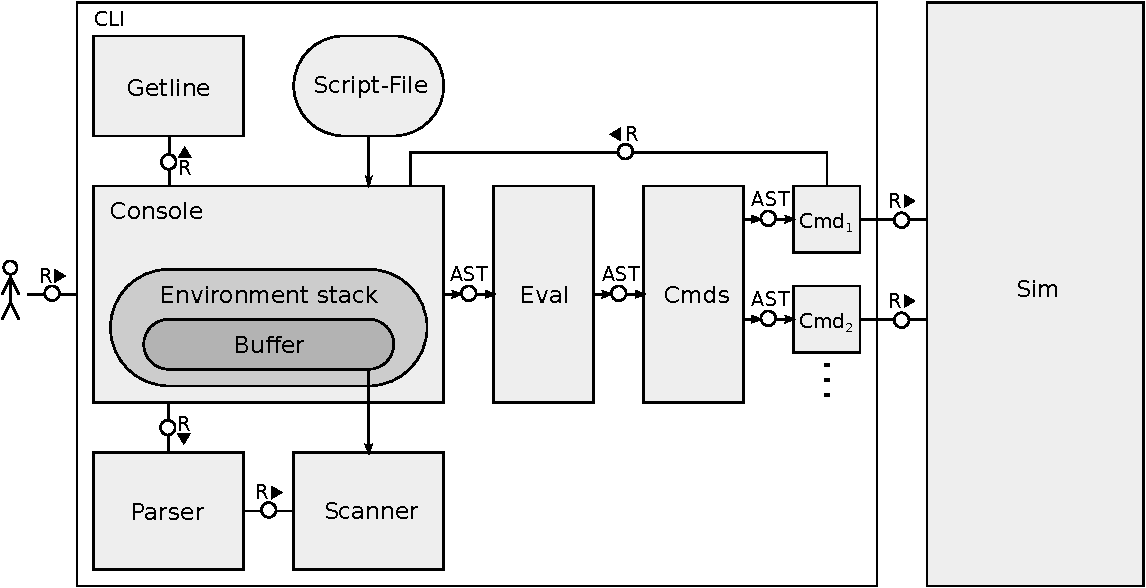
\includegraphics[width=\textwidth]{img/cli-fmc-crop.pdf}
	\caption{Architecture of the CLI in \protect\gls{FMC} notation}
\end{figure}
\noindent Conceptually, the user interacts with the CLI, whose main module is the \i{console}. Depending on whether the console is used interactively or not, it either uses the \i{getline} library\footnote{A small library, that allows basic line editing and provides a history, written by Chris Thewalt. It can be found in the folder \file{lib/getline} of GIMMIX.}  to read a line from the command line into the buffer or reads a specified script file into the buffer. Afterwards this input is parsed to construct an abstract syntax tree (\gls{AST}). The scanner and parser for this task have been generated by \gls{flex} and \gls{Bison}, respectively. As soon as the \gls{AST} is present, it is passed to the \i{eval} module, which executes it. If a node that represents a command is found, the module \i{cmds} comes into play. It holds a table with all available commands and will execute the corresponding function to execute the command. The commands will typically control the simulator, read the state or manipulate it.

As the FMC diagram indicates, the console manages a stack of \i{environments} to allow nesting. Each line or script execution will get a new environment on the top of the stack. This way, a command may use the console to execute a line or script as well. For example, the command \gcmd{tr} uses this feature by storing the desired command as a string and executing it later with the console.

\subsubsection{Command Infrastructure}

Because it is expected that the CLI language itself will not change much in future, but the commands will probably be changed and -- most important -- new ones will be added, it has been decided to separate cleanly between the language and the commands. Additionally, implementing and adding new commands should be as simple as possible. Similarly to the device infrastructure of GIMMIX, a compromise between dynamic and simplicity has been selected. That is, the module cmds keeps a table with all commands, but each command is implemented in its own file. Thus, to add a new command, a file has to be added and the table has to be extended.

Each command has an \i{execution function}, which receives the number of arguments and an array of \gls{AST} nodes -- one for each argument. Additionally, the cmds module provides the function `cmds_evalArg`:
\begin{lstlisting}[language=GIMMIXC]
sCmdArg cmds_evalArg(const sASTNode *arg,int expTypes,octa offset,bool *finished);
\end{lstlisting}
The function receives the argument to evaluate, the types that are supported (integer, float or string), an offset and a pointer to a boolean. The last two are used to implement ranges. Since the language is intended for scripting as well and it is imaginable that a user would like to, \eg, execute 1000 instructions and pipe the contents of the first 64 megabytes of memory into a file to analyze it with other tools later, it has been decided not to simply convert a range to an array. Because as the example shows, it might cost a lot of time and memory. Instead, the evaluation function receives the current offset and tells the caller whether all ranges are already finished. That means, in each step one value of each range is extracted, depending on the current offset.

The return value of `cmds_evalArg` is a struct called `sCmdArg`, that provides all required information about the value of the argument for the caller. It contains the type (integer, float or string), the origin (\gcmd{M8}, \gcmd{l}, \gcmd{\$}, and so on or an arbitrary expression such as \gcmd{1+2}), the location for origins like virtual memory or registers (that is, the memory address or register index) and of course the value of the argument as integer, float or string. The location and origin are for example used by \gcmd{p} to print the origin of an argument or by \gcmd{set} to set the corresponding entity of GIMMIX.

\subsubsection{Command Implementation}

A typical command, that makes use of ranges, is \i{disassemble}. Ignoring the details of the disassembling process, its implementation looks like the following:
\begin{lstlisting}[language=GIMMIXC,caption={Implementation of command \gcmd{d}}]
void cli_cmd_disasm(size_t argc,const sASTNode **argv) {
	if(argc > 1)
		cmds_throwEx(NULL);
	if(argc == 0) {
		for(int i = 0; i < DEFAULT_INSTR_COUNT; i++)
			doDisasm(cpu_getPC() + i * sizeof(tetra));
	}
	else {
		sCmdArg a;
		bool fin = false;
		for(octa off = 0; ; off += sizeof(tetra)) {
			a = cmds_evalArg(argv[0],ARGVAL_INT,off,&fin);
			if(fin)
				break;
			doDisasm(a.d.integer & -(octa)sizeof(tetra));
		}
	}
}
\end{lstlisting}
As the listing shows, at first the number of arguments is checked and if no arguments are given, `DEFAULT_INSTR_COUNT` (16) instructions at the PC will be disassembled. If one argument is given, `cmds_evalArg` will be called until `fin` has been set to `true`, whereas in each step the offset `off` will be increased to reach the next instruction. Thus, "\gcmd{d @:16}" would disassemble the instructions at addresses `@`, `@+4`, `@+8` and `@+12`.

Another interesting example, that utilizes the origin and location, is the command \gcmd{set}. The slightly shortened implementation is:
\begin{lstlisting}[language=GIMMIXC,caption={Implementation of command \gcmd{set}}]
void cli_cmd_set(size_t argc,const sASTNode **argv) {
	if(argc != 2)
		cmds_throwEx(NULL);
	for(octa off = 0; ; off++) {
		bool oFin = false, vFin = false;
		sCmdArg obj,val;
		obj = cmds_evalArg(argv[0],ARGVAL_INT,off,&oFin);
		val = cmds_evalArg(argv[1],
			ARGVAL_INT | ARGVAL_FLOAT,off,&vFin);
		if(oFin)
			break;

		switch(obj.origin) {
			case ORG_VMEM1:
				mmu_writeByte(obj.location,val.d.integer,0);
				break;
			...
			case ORG_EXPR:
				cmds_throwEx("Can't set arbitrary expr\n");
				break;
		}
	}
}
\end{lstlisting}
That means, it iterates over both the objects to set and the values at the same time, until the last object has been assigned. Additionally, the origin is used to determine what entity of GIMMIX should be changed. Of course, \gcmd{set} is not possible for expressions like \gcmd{1*2+M[0]} as first argument. It is only allowed for the \glslink{PC}{instruction pointer} and for fetches, that are specified without any operator in the "outmost layer", \ie \gcmd{M4[@+4]} for example.



\chapter{Test System}

As already mentioned in the introduction, it is very important that GIMMIX behaves correctly according to the MMIX specification. Additionally, since not all details are defined by the specification and to increase the confidence that everything has been understood and implemented correctly, the behaviour of GIMMIX is compared to the one of MMIX-SIM and MMIX-PIPE.

For this reason, a sophisticated test system has been built, that consists of two parts. At first, test programs for MMIX are executed on as many of the three simulators as possible and their results are compared. Second, \glslink{Unit testing}{unit tests} are used to test parts of GIMMIX, that are not visible to the software. This chapter describes the ideas behind both systems and the most important facilities that are required.

\section{Program Tests}

The basic idea behind the program tests is to let the simulators execute some instructions, that put values into registers and/or write to specific memory locations, and check afterwards if the registers and memory locations have the expected content.

\subsection{Test Infrastructure}

Each test consists of a \i{mms-file}, that holds the assembly code to test, and a \i{test-file}, that specifies the expected results. The first line of the test-file describes the values to compare, while the rest of the file is matched against the produced values. The first line is passed to the \i{post commands} module, which interprets it and prints the desired values. The line consists of an arbitrary number of commands, separated by ",". Each command can either be {\tt r:\dr{X}..\dr{Y}} to print dynamic registers \dr{X}, \dr{(X + 1)}, \dots, \dr{Y} or {\tt m:X..Y} to print the octas between physical memory addresses {\tt X} and {\tt Y}, inclusively.

MMIX-SIM, MMIX-PIPE and GIMMIX have been extended to support these post commands. They can be specified via command line argument to urge the simulator to execute them after the execution of the program is finished. This way, the contents of the specified registers or memory locations are printed to {\tt stdout}. GIMMIX provides the shellscript \file{runtests.sh}, that executes all test programs on the simulators, whereas the post commands are extracted from the first line of the test-file. Afterwards, the output of GIMMIX is compared to the expected output (all lines of the test-file, except the first one), to the output of MMIX-PIPE and to the output of MMIX-SIM. If there are any differences, the tool diff\footnote{Diff is a comparison utility, that finds and displays differences between two files. \citep{gldiff}} will be used to illustrate them. Additionally, it distinguishes between the following subfolders of folder \file{tests}, in which all program tests reside:
\begin{itemize}
	\item \file{user}: This directory contains tests, that can and should be executed in user mode. All three simulators have an option to execute a program in user mode, for which an initial environment is supplied. That is, \glslink{Paging}{paging} is pre-configured by setting \sr{V} and PTEs all installed for all four segments. Furthermore, \sr{S}, \sr{O}, \sr{K}, \sr{T} and \sr{TT} are initialized correspondingly. Most important, all tests in this folder are executable with all three simulators, \ie also with MMIX-SIM.
	\item \file{kernel}: This directory holds the tests, that should be executed in privileged mode. Therefore, they do not expect this initial environment, but start without any pre-configuration and in privileged mode. These tests are executed with MMIX-PIPE and GIMMIX only.
	\item \file{diff}: To test some behaviours that are implementation-defined, to test the fix for the page fault problem on the stack or to test cases that are currently erroneous in MMIX-PIPE or MMIX-SIM, the folder \file{diff} is used. All tests in it are executed on GIMMIX only.
	\item \file{cli}: Finally, this directory holds tests for the command line interface. Thus, the tests are typically no programs for MMIX, but scripts for the CLI. Of course, they are executed in GIMMIX only.
\end{itemize}
All other folders are ignored by \file{runtests.sh}. But it is noteworthy, that the folder \file{manual} holds some programs for GIMMIX, that make use of the yet existing devices. These are not included into the program test system, because they are not automatically testable that easily.

\subsection{Test Programs}

Although the tests programs can not be explained in detail, this section will give an overview about them.

\subsubsection{User Tests}

Since all three simulators can execute the user tests, as many cases as possible are tested in this way. Most of them simply test the behaviour of a set of instructions. While a part of the tests have been written manually, all tests, in which the individual test cases work in a common pattern, are generated by scripts or programs. All these generators are placed in the directory \file{testgen}, which contains two groups of generators. The first group are \gls{Ruby} scripts, that are used for most of the tests. \gls{Ruby} has been chosen, because it allows a quick development of the tests and provides an arbitrary-precision arithmetic, independend of the underlying platform (in other scripting languages, such as \gls{PHP}, the width of integers depends on the platform, on which the interpreter runs \citep{php-intwidth}). This way, \eg bit operations with 64-bit integers can be performed, regardless of whether the generator is run on a 32-bit or 64-bit platform. The second group are C programs, that are primarily used for the floating point arithmetic tests. Because this way, the double precision arithmetic of a well tested language and platform can be utilized to make sure, that the implementation of the floating point instructions in GIMMIX is correct. \gls{Ruby} is not well suited in this case, because of the arbitrary precision arithmetic; instead C fits better, because of the amount of control and the similarities of double precision arithmetic and 64-bit float arithmetic in MMIX. Additionally it is noteworthy, that some of these test generators expect x86 as underlying platform, because the rounding mode of the x87 floating point unit is set and some reactions on not defined details by IEEE-754 and therefore x87-specific behaviour are necessary. For example, the sign-bit of \NaN results is not defined by the standard \citep[pg. 17]{ieee754}.

\subsubsection{Kernel Tests}

Most of the tests in the \file{kernel} directory have been written manually. They test the PEs of MMIX, \glslink{Interrupt}{interrupts}, \glslink{Paging}{paging} and privileged instructions. But some of them are generated automatically as well. Most important, the \glslink{Paging}{paging} tests are generated automatically with a \gls{Ruby} script, that generates PTPs, PTEs and access tests for a given value of \sr{V}.

\subsubsection{Diff Tests}

As already mentioned, MMIX-PIPE and GIMMIX differ in a few details. For example, the values of \sr{XX}, \sr{YY} and \sr{ZZ} are not equal for some \glslink{Exception}{PEs}, because MMIX does not define it completely. Another example is, that GIMMIX will trigger an \glslink{Exception}{exception} if a not existing memory location in the I/O space is accessed or a bit in \sr{Q} is set, that is not used for an \glslink{Interrupt}{interrupt}, \glslink{Exception}{PE} or \glslink{Exception}{ME}, while MMIX-PIPE will not do that. The second reason for this directory is, that the fix for the page fault problem on the stack has to be tested, which of course does not work in MMIX-PIPE.

\subsubsection{CLI Tests}

Finally, the directory \file{cli} contains scripts to test the language and commands of the CLI. In this case, obviously, the expected results are only compared with the actual results. Currently, the expressions of the language, handling of whitespace and the most critical and important commands such as \gcmd{p}, \gcmd{set}, \gcmd{e}, \gcmd{b}, \gcmd{d}, \gcmd{tr} and a few others are tested.

\subsection{Code Coverage}

To ensure that all lines in the important parts of the simulator are executed by the tests, a small code coverage system has been developed. The basic functional principle is to cause \gls{gcc} to let the simulator generate information for gcov\footnote{Gcov is a test coverage program, that can be used together with \gls{gcc} to improve the performance of a program and discover untested parts of it. \citep{gcov}} during the execution of the simulator. The shellscript \file{runcov.sh} runs the simulator for a specific or for all tests and uses gcov to produce the coverage information. This information is analyzed by a few \gls{Ruby} scripts to generate HTML pages, that display the results. These pages contain a list of all tests, whereas each of them displays the source files of the simulator with the percentage of executed lines. Additionally, one HTML page per source file is generated, displaying the source code and highlighting the lines correspondingly, depending on whether they have been executed or not.

\section{Unit Tests}

The second part of the test system consists of \glslink{Unit testing}{unit tests}. As already said, they are used to test the parts of GIMMIX, that are not visible to the software or would be difficult to test. To achieve that, a small \glslink{Unit testing}{unit test} framework has been developed. Although existing frameworks like CUnit\footnote{Available at \url{http://cunit.sourceforge.net}.} or Check\footnote{Available at \url{http://check.sourceforge.net}.} have been considered, it has been decided to built an own framework, because the existing ones are quite heavy and most of their functionality would not be used anyway. Additionally, of course they do not provide special functions to compare bytes, wydes, tetras and octas. Thus, by building our own framework, it can be designed to fit our needs exactly.

The test framework found in \file{unittests/test.c} allows it to register and run tests, and offers functions to assert equalities. The function `test_register` is intended to register a \i{test suite}, which contains one or more \i{test cases}. Each test case has a name and a function, that runs that test case. After registering all test suites, `test_start` can be called to execute all test cases in all test suites. To support a convenient and informative facility for asserts, it offers the macros `test_assertTrue`, `test_assertInt`, `test_assertByte`, `test_assertOcta` and so on, which call the actual assert function with the current function name and line number. This way, reasons of failures can be identified and fixed more quickly.

Currently, tests suites exist for testing the physical memory (independent of the rest of the memory hierarchy), the complete memory hierarchy (focused on the different flags such as `MEM_UNCACHED` or `MEM_SIDE_EFFECTS`), the system instructions like \mi{LDUNC}, \mi{SYNCD}, \mi{SYNC} and so on and the interruptibility of instructions.


\chapter{Future Possibilities}

The current state of the GIMMIX project is, as described in the previous chapters, that the simulator itself including a few basic devices is completely finished. That is, the simulator realizes the entire MMIX architecture. Additionally, a convenient and powerful command line interface exists and the whole system has been tested as much as possible to reach the confidence, that everything works as intended. This final chapter mentions yet missing parts to reach the goal of porting an operating system to MMIX and suggests a few possible enhancements.

\section{Missing Parts for an Operating System Port}

At first, the yet missing tools and changes for developing or porting an operating system for MMIX are listed.

\subsection{\mi{TRAP 0,0,0} halts the Simulator}

To allow automatized tests, the simulator has to be stoppable in some way. Since MMIX-SIM uses a \mi{TRAP} with only zeros as arguments for a quit command, GIMMIX does so as well. Additionally, MMIX-PIPE has been changed, so that it stops for \mi{TRAP 0,0,0}, too. Of course, this is only temporary, because MMIX defines that a \mi{TRAP 0,0,0} terminates a user process. That is, the operating system should handle that trap -- like all others as well -- and the simulator should not stop. Hence, to be able to develop or port an operating system, this "feature" has to be removed or replaced with something else.

\subsection{Toolchain}

Currently, GIMMIX does not provide its own assembler and has no C compiler and linker at all. Instead, it uses the assembler \i{mmixal}, written by Donald Knuth, to produce special MMIX object files. These in turn are converted by a tool to an ASCII file, that specifies which values should be written to which physical memory addresses. GIMMIX interprets this format to load a program into the main memory. Of course, this is only a temporary solution. Later, a ROM should be put into the simulator, which initiates the boot process. Although it is imaginable that programs can still be loaded directly into GIMMIX for testing purposes, these will probably not be specified in that ASCII format, but in a binary format. MMIX-PIPE understands the ASCII format as well and MMIX-SIM is able to load the MMIX object files, which is one of the reasons why GIMMIX uses this solution currently.

As already mentioned, the project uses no C compiler yet. By now, a GNU toolchain (\gls{gcc} cross-compiler, binutils\footnote{GNU binutils is a collection of tools for analyzing binary files, building archives or stripping symbols from a file \citep{binutils}.} and newlib\footnote{Newlib is a small C library, that is intended for embedded systems \citep{newlib}.}) for MMIX\footnote{The GNU toolchain is available at \url{http://www.bitrange.com/mmix}.} is already available due to the efforts of Hans-Peter Nilsson, which could be used in future. Another opportunity would be to build a backend for the lcc\footnote{Lcc is a retarget compiler for ANSI C \citep{lcc}.}, which has already been started in the previous GIMMIX approach, but is not yet finished.

\subsection{Startup and Tools}

Although GIMMIX already provides a ROM and a disk device, tools for disk creation, partitioning, filesystem creation and so on are still missing. The previously mentioned project ECO32 offers tools for such tasks, which could be used for GIMMIX as well.

\section{Extensions and Enhancements}

As mentioned, the simulator is considered complete, but there are of course still imaginable improvements and additional features. These are listed in this section.

\subsection{More Devices}

The currently provided devices are only the basic ones, which have been added primarily to ensure that the device infrastructure is sufficient. Therefore, a few more will have to be added in future. For example, every reasonable operating system will need a screen and a keyboard, instead or additional to the already existing terminals. Furthermore, a real-time clock would be a useful device. A screen and a keyboard are for example present in the ECO32 project and could thus be ported to GIMMIX.

\subsection{Working with Symbols in the CLI}

Since the loading format used in GIMMIX is not considered final, the CLI does not offer the opportunity to use symbols instead of addresses at the moment. That is, for example breakpoints can only be set by specifying virtual or physical addresses, but not via symbols, that have been assigned to virtual addresses. Of course, this would simplify the debugging process.

\subsection{Interface to \protect\gls{GDB}}

As soon as programs for MMIX can be written in C, for example, it would be more convenient to debug such programs in the language they have been written in, instead of having to work with the generated assembly. To do so, GIMMIX could provide an interface for \gls{GDB}, that offers the opportunity to control GIMMIX with \gls{GDB}. Fortunatly, an alpha version of \gls{GDB} for MMIX\footnote{The complete GNU toolchain for MMIX including \gls{GDB} is available at \url{http://math.cs.hm.edu/mmix/examples/MMIXonMMIX/index.html}.} is already available because of the work of Mr. Ruckert. Therefore, as soon as the \gls{GDB} interface in GIMMIX is present, it should be possible to use that version of \gls{GDB} to debug programs running on GIMMIX.

\subsection{Infrastructure for MMIX Programs without OS}

To be able to run all example programs for MMIX -- especially those that are or will be listed in the volumns of the \gls{The Art of Computer Programming} books about MMIX  -- directly in GIMMIX, \ie without an operating system, a few additions to GIMMIX are necessary. These are:
\begin{itemize}
	\item Those programs expect a rudimentary operating system, that provides special system calls via forced traps to perform I/O requests. That is, opening a file, reading a file, writing to a file and so on, which can for example be used to write to {\tt stdout} or read from {\tt stdin}. In contrary to GIMMIX, MMIX-SIM and MMIX-PIPE offer these system calls.
	\item Additionally, mmixal allows it to pre-allocate global registers and initialize them with specific values. This feature is currently not usable, because the ASCII file format does not support that. MMIX-SIM (and MMIX-PIPE, when started in user mode), for example, starts with the instruction \mi{UNSAVE} to establish a part of the user environment, including the requested global registers.
	\item To allow more interaction with the host platform, MMIX-SIM provides the number of arguments, given to itself, in \dr{0} and a pointer to the first one in \dr{1}. Additionally, feedback can be passed back by putting a value in \dr{255}, which will be returned by the main function of MMIX-SIM.
\end{itemize}
These features are not present in GIMMIX at the moment, because it has a different goal than MMIX-SIM and MMIX-PIPE. Nevertheless, it might make sense to provide such facilities as well, \eg requested by a command line argument, to allow the execution of all the programs for MMIX, that require them.

\subsection{Acid Test Mode}

When developing or porting an operating system, a deterministic machine is appreciated in most cases. That means, that the behaviour of the machine is always exactly the same, when the start conditions do not change. This is especially a problem when working with real hardware, because for example the timing of devices varies. Of course, a deterministic behaviour simplifies debugging, since errors are reproducible. But in some cases, it might be helpful to produce non-deterministic behaviour or random start conditions on purpose, to make sure that the OS works correctly in these cases as well or to detect errors, that would not have arisen otherwise. GIMMIX could help by providing an "acid test mode", which initializes registers, main memory and so on with random values, randomizes the timing behaviour of devices or similar.

\subsection{Graphical User Interface}

As already mentioned, a graphical user interface for GIMMIX could be provided. Since the simulator core is completely independent of the current command line interface, it could be easily exchanged with a GUI or both could coexist. A GUI would have the advantage, that many entities of MMIX such as the dynamic registers, special registers, main memory and so on could be displayed simultaneously. Additionally, the disassembly of the previous and next few instructions could be displayed as well. Thus, it would allow a more productive interaction with the simulator.

\subsection{Provide Information about Hardware for Software}

Currently, operating systems for MMIX are very dependent on the particular MMIX implementation they are designed for. Because, the devices, the amount of main memory, the cache configuration and so on, is either not investigatable at all or only with a lot of effort. Therefore, it could make sense to add a kind of "meta-device", that provides that information at specific addresses in the I/O space. This way, the OS could react dynamically on present devices, find out the amount of main memory easily and make more efficient use of caches. Of course, this meta-device should be part of the MMIX specification, so that all MMIX implementations provide it.

\subsection{Mapping of the I/O Space}

Unfortunatly, at the moment MMIX does not allow to map the I/O space via paging. That is, the I/O space can only be accessed in privileged mode by using the directly mapped space. The reason is, that the physical address in a PTE is only 48 bit wyde, which does not include the I/O space. This will be a problem for microkernel operating systems, because it is not possible to implement drivers as user processes. A solution might be to limit the I/O space to range from \haddro{0001}{0000}{0000}{0000} to \haddro{00FF}{FFFF}{FFFF}{FFFF} and extend the width of the physical address in a PTE to 56 bits. This way, the upper 8 bits of a PTE would still remain for the operating system and the I/O space should still be large enough as well. Additionally, the width of a translation in the TCs would have to be extended. These changes would allow the operating system to map pages from the I/O space into the user space, so that user processes can access it.



\printglossary

\addcontentsline{toc}{chapter}{Listings}
\lstlistoflistings

\addcontentsline{toc}{chapter}{Bibliography}
\bibliography{bibliography}

\addcontentsline{toc}{chapter}{Eidesstattliche Erklärung}
\chapter*{Eidesstattliche Erklärung}

Hiermit versichere ich, die vorliegende Arbeit selbstständig und unter
ausschließlicher Verwendung der angegebenen Literatur und Hilfsmittel erstellt
zu haben.

\paragraph{}
Die Arbeit wurde bisher in gleicher oder ähnlicher Form keiner anderen
Prüfungs-behörde vorgelegt und auch nicht veröffentlicht.\\[2cm]
Marburg, \today


\end{document}
